%%Introduction

In this Section, we consider models with a photon, a W boson, a Z boson or a Higgs boson in the final state,
accompanied by Dark Matter particles that either couple directly to the boson or are mediated by
a new particle. The experimental signature is identified as \textit{V+MET}.

These models are interesting both as some are demanded by gauge coupling relations in models where the gluon provides
the experimentally detectable signature,
and also as stand-alone models with final states that cannot be generated by the models in
Section~\ref{subsec:MonojetLikeModels}.

%%%Classification of models


%
The models considered can be divided into three categories:
\begin{description}
% \item[Models including a contact operator, where the boson is radiated from the initial state] As depicted in
% the left diagram of Figure~\ref{fig:VPlusMET_EFT}, these models follow the nomenclature and theory
% for the EFT benchmarks commonly used by MET+X searches~\cite{Goodman:2010ku}. These models
% have been used in past experimental searches~\cite{Khachatryan:2014rwa, Aad:2014vka,Khachatryan:2014tva, Aad:2014vka,
% ATLAS:2014wra, Aad:2013oja}, and they will not be described here.
 \item[Simplified models with a boson radiated either from the initial state or from the mediator] These models follow those
 already described in Section~\ref{subsec:MonojetLikeModels}, replacing the gluon with a boson.
  \item[V-specific simplified models] These models postulate direct couplings of new mediators
 to bosons, e.g. they couple the Higgs boson to a new vector or to a new scalar~\cite{Carpenter:2013xra,Berlin:2014cfa}. 
 \item[Models including a contact operator, where the boson is directly coupled to DM]
 Shown on the right-hand side of Figure~\ref{fig:VPlusMET_EFT},
 these models allow for a contact interaction vertex that directly couples the boson to Dark Matter~\cite{Cotta:2012nj, Carpenter:2012rg, Crivellin:2015wva,Berlin:2014cfa}.
 These models are included in this report devoted to simplified models since 
 UV completions for most of these operators proceed through loops and are not available to date. 
 These models provide a benchmark to motivate signal regions that are unique to searches with
 EW final states and would otherwise not be studied. However, we recommend to use these models
 as placeholders and emphasize model-independent results especially in signal regions tailored to these models. 
 Wherever results are interpreted in terms of these operators, a truncation procedure
 to ensure the validity of the EFT should be employed, as detailed in Section~\ref{sec:EFTValidity}. 
\end{description}

\begin{figure}[h!]
	\centering
	\vspace{\baselineskip}
	\unitlength=0.0045\textwidth
%	\begin{feynmandiagram}[modelVisr]
%		\fmfleft{i1,i2}
%		\fmfright{o1,o2}
%		\fmftop{isr}
%		\fmfbottom{pisr}
%		\fmfv{decor.shape=circle,decor.filled=shaded, decor.size=30}{v1}
%		\fmf{fermion}{o2,v1,o1}
%		\fmf{fermion}{i2,visr,v1}
%		\fmf{plain}{v1,pvisr,i1}
%		\fmf{fermion,tension=0}{v1,i1}
%		\fmflabel{\Large ${\bar{q}}$}{i1}
%		\fmflabel{\Large ${q}$}{i2}
%		\fmflabel{\Large ${\bar{\chiDM}}$}{o1}
%		\fmflabel{\Large ${\chiDM}$}{o2}
%		\fmf{photon,tension=0}{visr,isr}
%		\fmf{phantom,tension=0}{pvisr,pisr}
%		\fmflabel{\Large ${V}$}{isr}
%	\end{feynmandiagram}
	\begin{feynmandiagram}[modelVeft5pt]
		\fmfleft{i1,i2}
		\fmfright{o1,o2,o3}
		\fmf{photon,label={\Large $V$}}{v1,v2}
		\fmfv{decor.shape=circle,decor.filled=shaded, decor.size=30}{v2}
		\fmf{fermion}{i2,v1,i1}
		\fmf{fermion}{o2,v2,o1}
		\fmflabel{\Large ${\bar{q}}$}{i1}
		\fmflabel{\Large ${q}$}{i2}
		\fmflabel{\Large ${\bar{\chiDM}}$}{o1}
		\fmflabel{\Large ${\chiDM}$}{o2}
		\fmf{photon}{o3,v2}
		\fmflabel{\Large ${V}$}{o3}
	\end{feynmandiagram}
	
	\vspace{\baselineskip}
	\caption{Sketch of benchmark models including a contact interaction
		for V+MET searches, adapted from~\cite{Nelson:2013pqa}. \label{fig:VPlusMET_EFT}}
\end{figure}

The following Sections describe the models within these categories,
the parameters for each of the benchmark models chosen,
the studies towards the choices of the parameters to be scanned.

\section{Simplified models with boson radiation} \label{sec:bosonrad}
\svnidlong
{$HeadURL: $}
{$LastChangedDate: $}
{$LastChangedRevision: $}
{$LastChangedBy: $}
\svnid{$Id: $}   


Monojet searches are generally more sensitive
with respect to final states including bosons, due to the much
larger rates of signal events featuring quark or gluon radiation with
respect to radiation of bosons~\cite{Zhou:2013fla},
in combination with the low branching ratios if leptons from
boson decays are required in the final state.
The rates for the Higgs boson radiation is too low for these models
to be considered a viable benchmark~\cite{Carpenter:2013xra}.
However, the presence of photons,
leptons from W and Z decays,
and W or Z bosons decaying hadronically
allow backgrounds to be rejected more effectively,
making Z/gamma/W+\MET searches
still worth comparing with searches in the jet+\MET final state.
\Todo{Additional motivations exist for this final state from SUSY searches.}
%TODO: Linda is writing sentence to make this stronger. 

% The three commonly chosen EFT benchmarks for Dirac dark matter that are
% kinematically distinct for what concerns the observables used in
% \MET+X searches~\footnote{[CD: we would need a plot here, or a reference to
% monojet section where this is shown]} and span a wide range of \MET spectrum in
% the boson+\MET searches are, in the notation of ~\cite{Goodman:2010ku},
% the D1 (scalar SM/WIMP interaction), D5 (vector-vector interaction) and D9
% (tensor interaction) operator.

\subsection{Vector mediator exchanged in the \schannel}

An example Feynman diagram for these processes can be constructed by taking
Fig.~\ref{fig:OP} and replacing the gluon with $\gamma,W$ or $Z$.
The interest for searches with W bosons in the final state
has been elevated by the increased cross section
for certain choices of couplings for a spin-1 mediator~\cite{Bai:2012xg}.
Run-1 searches have considered three sample cases for the product of
up and down quark couplings to the mediator, denoted as $\xi$:
\begin{itemize}
 \item No couplings between mediator and either up or down quarks~($\xi=0$);
 \item Same coupling between mediator and each of the quark types~ ($\xi=1$);
 \item Coupling of opposite sign between mediator and each of the quark types~($\xi=-1$).
\end{itemize}
The $\xi=-1$ case leads to a large increase in the cross-section of the process,
and modifies the spectrum of missing transverse energy or
transverse mass used for the searches. The sensitivity of the W+\MET search for
this benchmark in this case surpasses that of the jet+\MET search.
However, as shown in Ref.~\cite{Bell:2015sza}, the cross-section increase is due
to the production of longitudinally polarized W bosons,
as a consequence of a violation of electroweak gauge symmetries. Unless further
particles are introduced (in a fashion similar
to the Higgs boson in the Standard Model), choosing a value of $\xi=-1$
for this simplified model will lead to a manifest violation of unitarity at LHC energies.
The simplified model with a vector mediator exchanged in the \schannel model
can still be considered as a benchmark for searches with a W boson if $\xi=1$.
We leave the study of further models with cross-section enhancements due
to different couplings to up and down quarks for studies beyond the early LHC searches
covered in this document.
An example of such model is the case of both DM and SM Higgs charged under a new $U(1)'$,
with a a small mass mixing between SM Z-boson and the new \Zprime. This leads
to different effective DM couplings to $u_L$ and $d_L$, proportional to
their coupling to the Z boson, detailed in Appendix~\ref{app:EWSpecificModels_Appendix}.

The scan in the parameters that characterize this simplified model for EW boson + \MET
searches follow what is
already detailed in Section~\ref{subsec:MonojetLikeModels}.
%FIXME: refer to appropriate subsection

% CD: I tend to like this list so I'll leave it here in hope of recycling it
% \begin{itemize}
%  \item the mass of the DM particle ($m_{DM}$);
%  \item the mediator mass ($m_{Med}$);
%  \item the mediator width ($\Gamma_{Med}$);
%  \item the couplings between the DM and the mediator (\gdm),
%  and between the mediator and the initial state quarks ($g_{SM}$);
%  \item the chirality of the couplings between DM and mediator,
%  and between mediator and initial state quarks (vector-vector, axial-vector, axial-axial, vector-axial).
% \end{itemize}

As in the case of the jet+\MET models, the width does not have a significant
impact on the kinematic distributions relevant for those searches. An example
of the particle-level analysis acceptance using the
generator-level cuts from Ref.~\cite{Aad:2014tda}
for the photon+\MET analysis, but raising the photon $p_T$ cut
to 150~\gev is shown in Figure~\ref{fig:DMV_EW_gamma_acceptance},
comparing a width that is set to $\Gamma=M_{med}/3$ to the
minimal width (the ratio between the two widths
ranges from 1.05 to 1.5 with increasing mediator masses).

%% Redone as a table.
% mmed : minW
% 10  : 3.5
% 50 : 21.3
% 100 : 42.4
% 300 : 127.3
% 600 : 300.1
% 1000 : 503
% 3000 : 1512
% 6000 : 3024
\begin{table}[!h]
\begin{tabular}{| l |r r r r|}\hline
\multicolumn{5}{|c|}{Acceptance ratio for $\Gamma=\Gamma_{\rm min}$ vs
$\Gamma=\mMed/3$} \\ \hline 
\multicolumn{1}{|c|}{ } & \multicolumn{4}{c|}{\mdm/GeV}\\
\hline 
{\mMed/GeV}      & 10     & 50    & 200   & 400  \\ \hline
50   & 0.96   & 0.99  &       & 0.95 \\  
100  & 0.97   &       &       &      \\
300  & 1.00   & 1.02  &       &      \\
600  &        &       & 0.96  &      \\
1000 & 1.01   & 1.02  & 1.03  &      \\
3000 & 1.02   & 1.03  &       & 1.01 \\
\hline
\end{tabular}
    \caption{Analysis acceptance for the photon+\MET analysis when varying the mediator width, in the
    case of a vector mediator exchanged in the $s-$channel}%This plot will come from Marie-Helene
    \label{fig:DMV_EW_gamma_acceptance}
\end{table}

%% \begin{figure}
%%     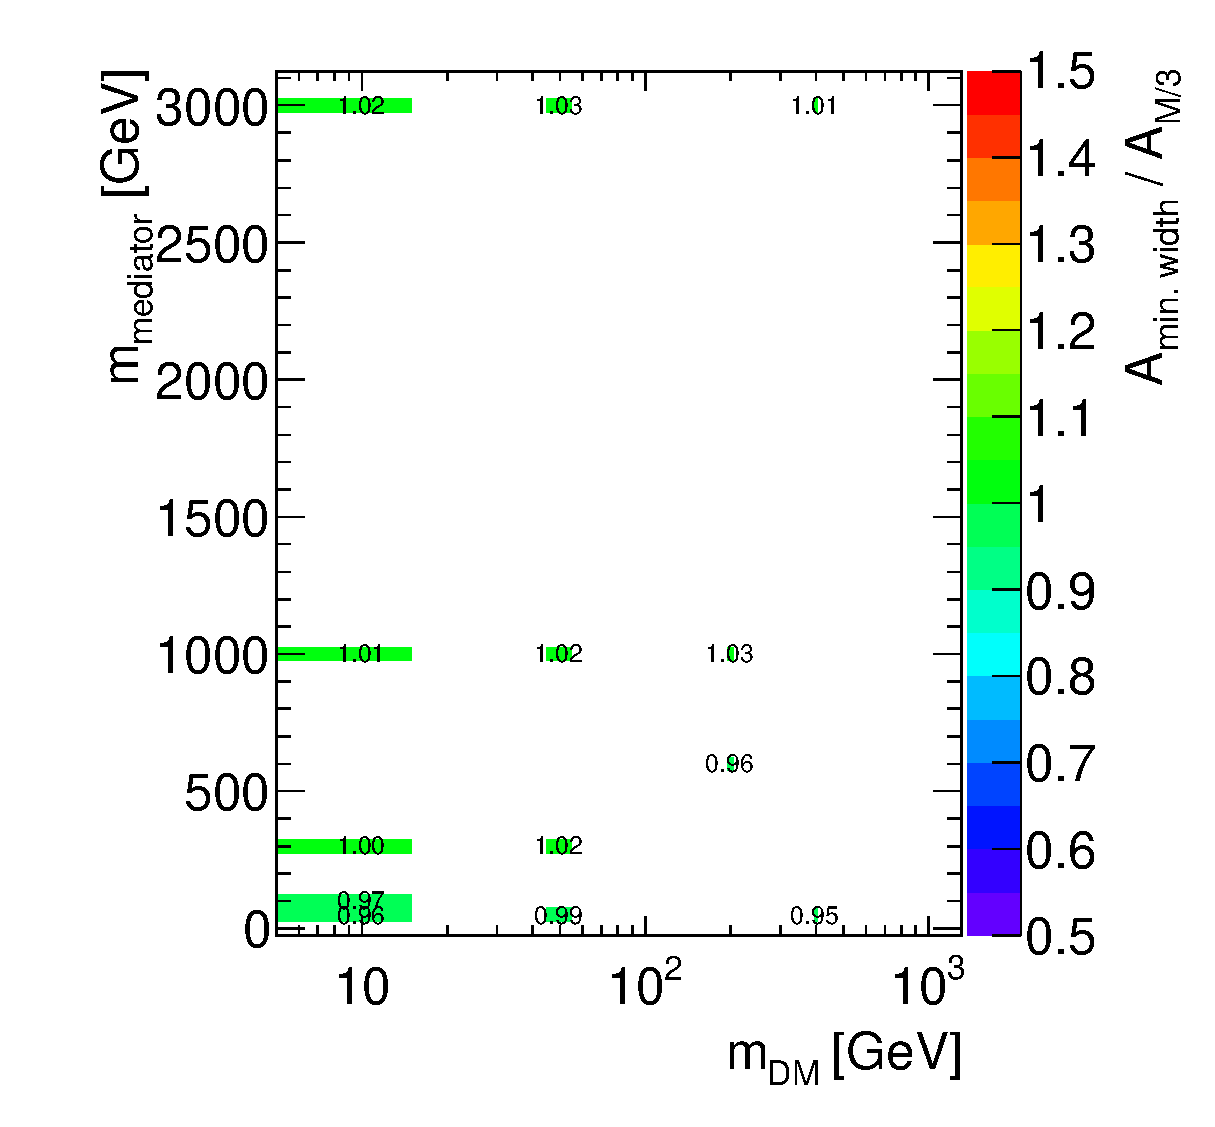
\includegraphics[width=0.7\textwidth]{figures/EW/acceptance_minwidth_vs_mo3_gamma}
%%     \caption{Analysis acceptance for the photon+\MET analysis when varying the mediator width, in the
%%     case of a vector mediator exchanged in the $s-$channel}%This plot will come from Marie-Helene
%%     \label{fig:DMV_EW_gamma_acceptance}
%% \end{figure}

Examples of relevant kinematic distributions for selected benchmark points are
shown in Fig.~\ref{fig:DMV_EW_kinematics_SVMed}. 
leading-order cross-sections for the chosen 
benchmark points are shown in Appendix~\ref{app:EWSpecificModels_Appendix}.

\begin{figure}[h!]
\centering  
\subfloat[Missing transverse momentum distribution for the photon+\MET final state, for 
different mediator mass choices, for \mdm=10~\gev.\label{fig:DMV_EW_gamma_MET_SVMed}]{%
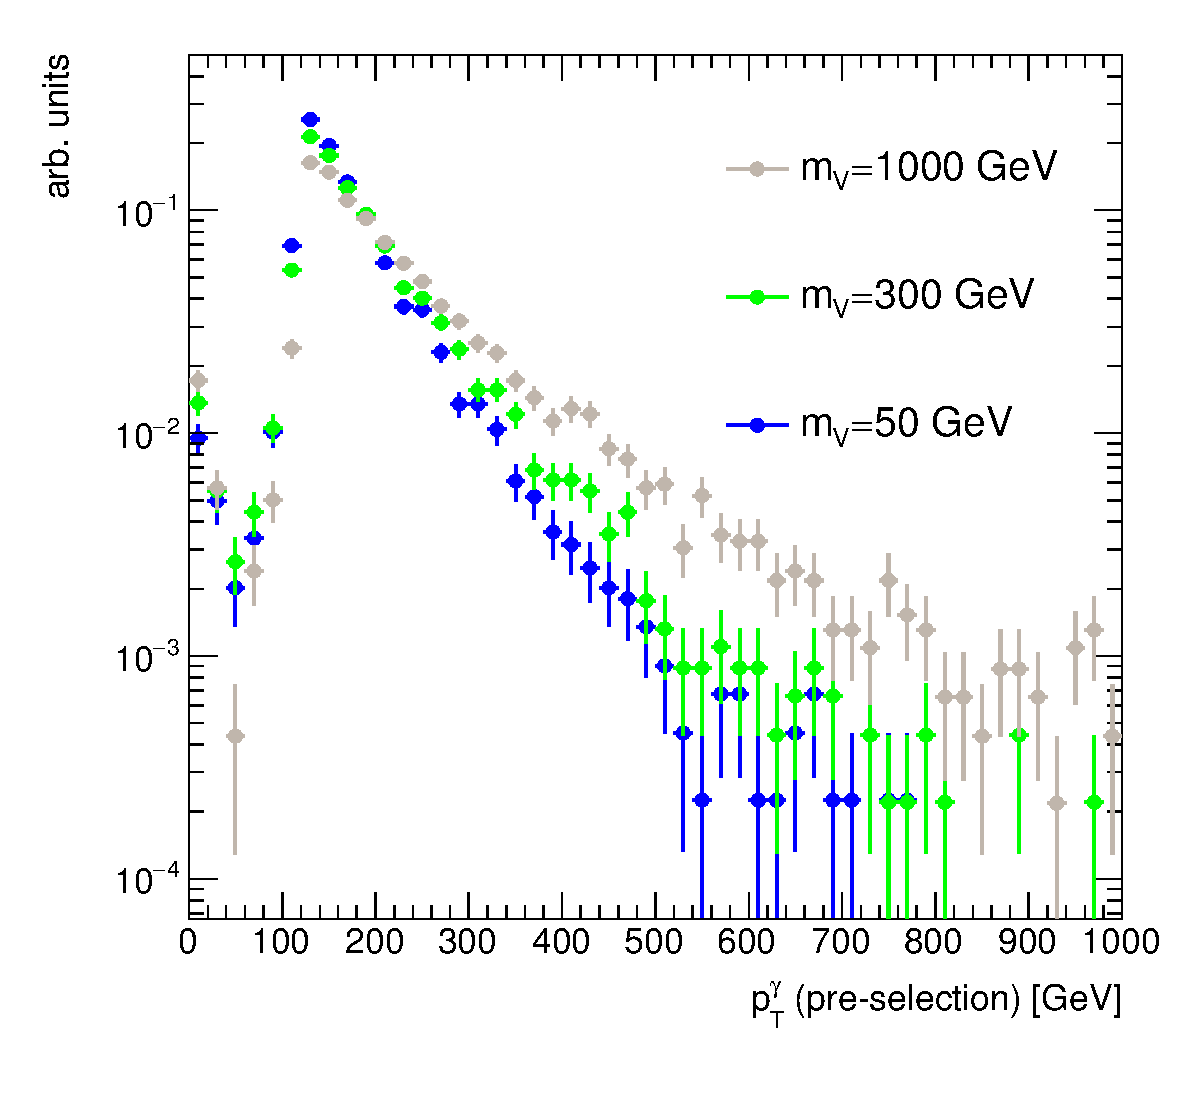
\includegraphics[width=0.45\textwidth]{figures/EW/ptGamma_filter120GeV_dmV_dm10GeV}
}%TODO: add this + equivalent plot of \MET to appendix
\hfill
\subfloat[Leading photon transverse momentum distribution for the photon+\MET final state, 
for different DM mass choices, with \mMed=1~\tev.\label{fig:DMV_EW_gamma_pT_SVMed}]{%
		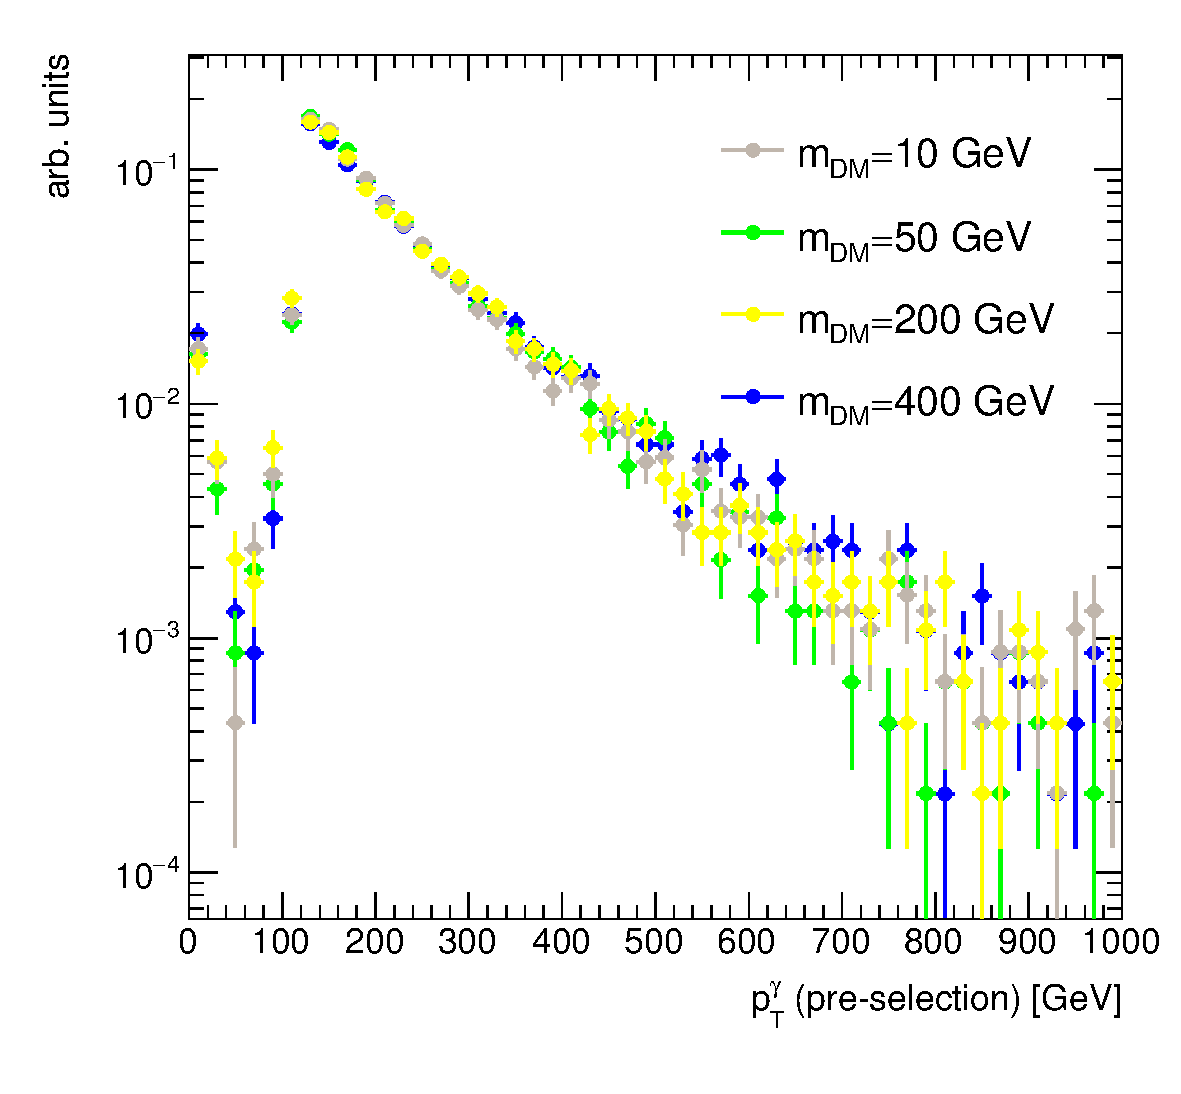
\includegraphics[width=0.45\textwidth]{figures/EW/ptGamma_filter120GeV_dmV_mV1000GeV}
}%TODO: add equivalent plot of \MET to appendix
\hfill
\subfloat[Missing transverse momentum distribution for the leptonic Z+\MET final state, 
for different mediator mass choices, for \mdm=15~\gev\label{fig:DMV_EW_Z_MET_SVMed}]{%
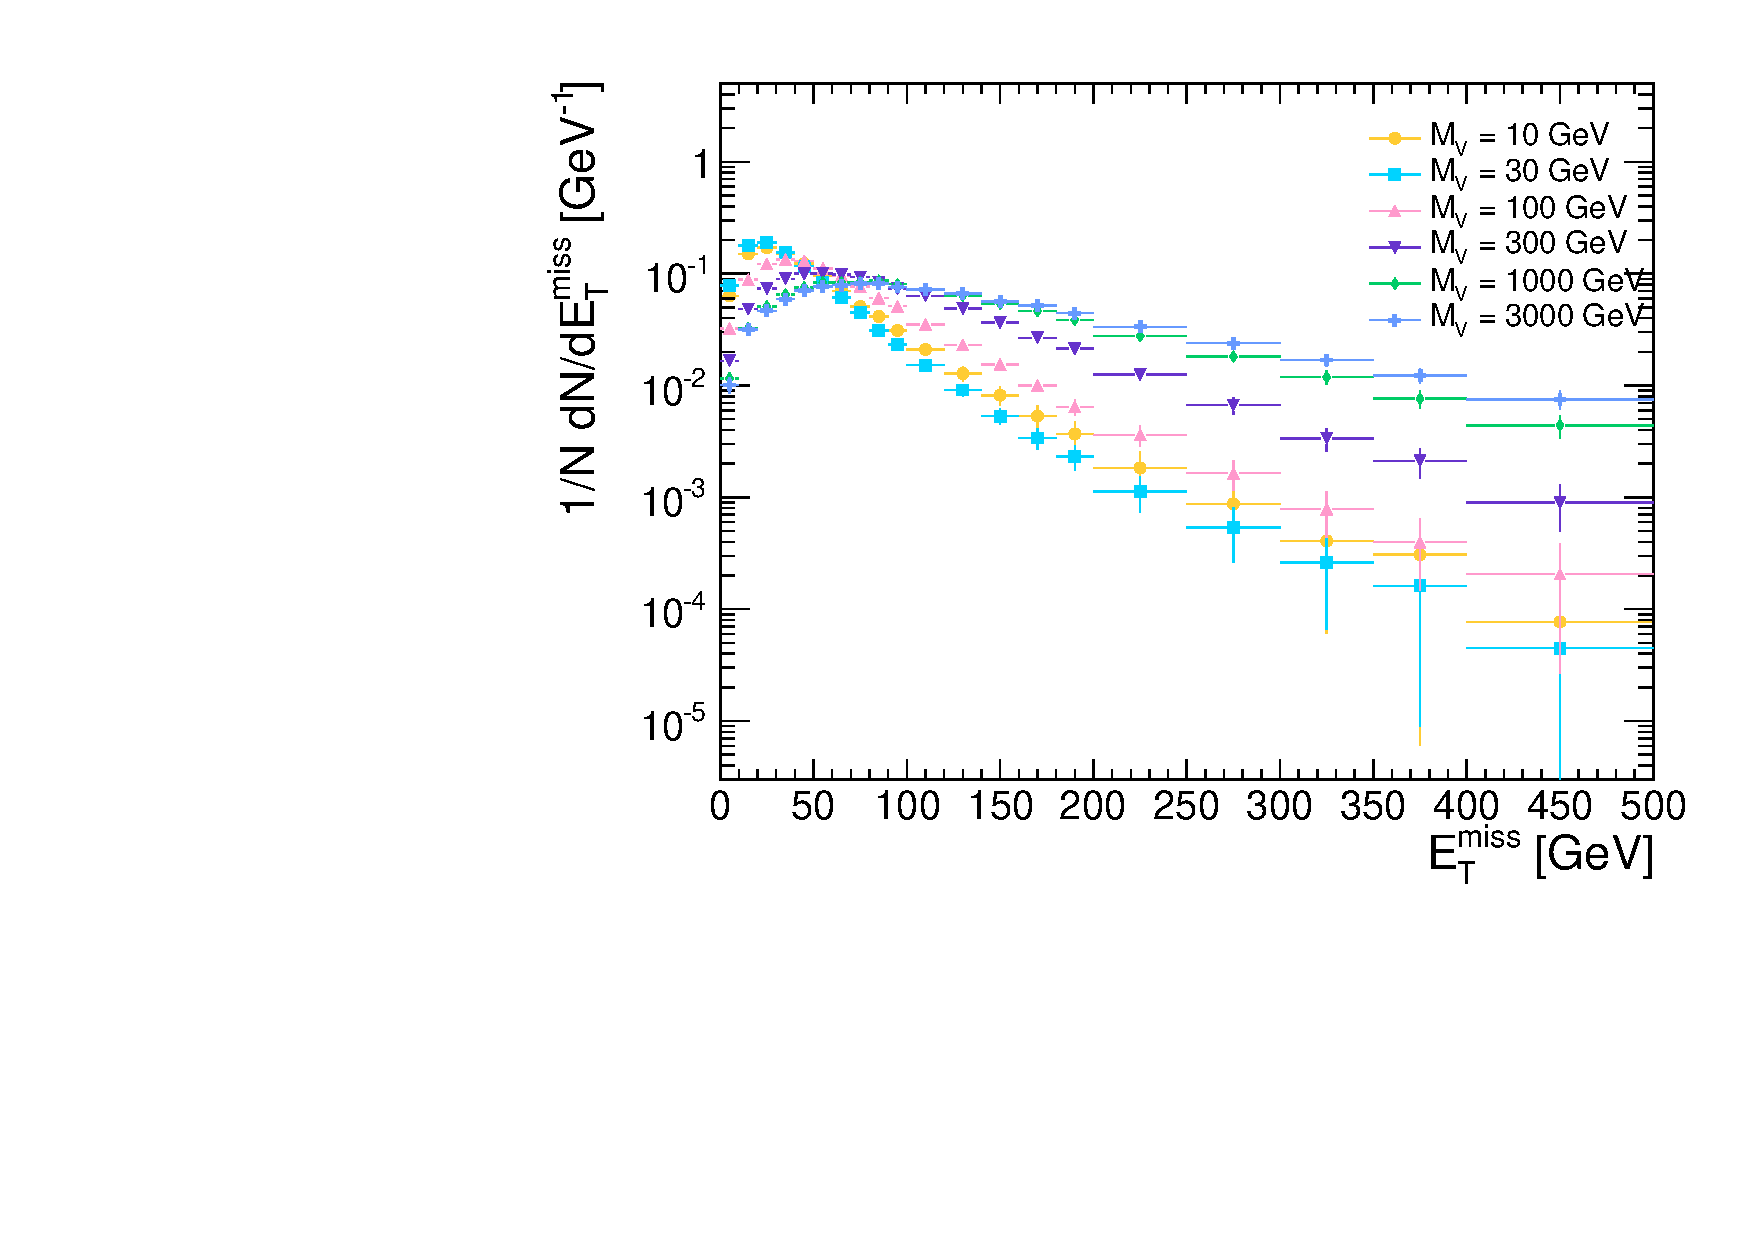
\includegraphics[width=0.45\textwidth]{figures/EW/pt_vv_Mx15}
}    
\hfill
\subfloat[Missing transverse momentum distribution for the hadronic W+\MET final state.\label{fig:DMV_EW_Whad_MET_SVMed}]{%
	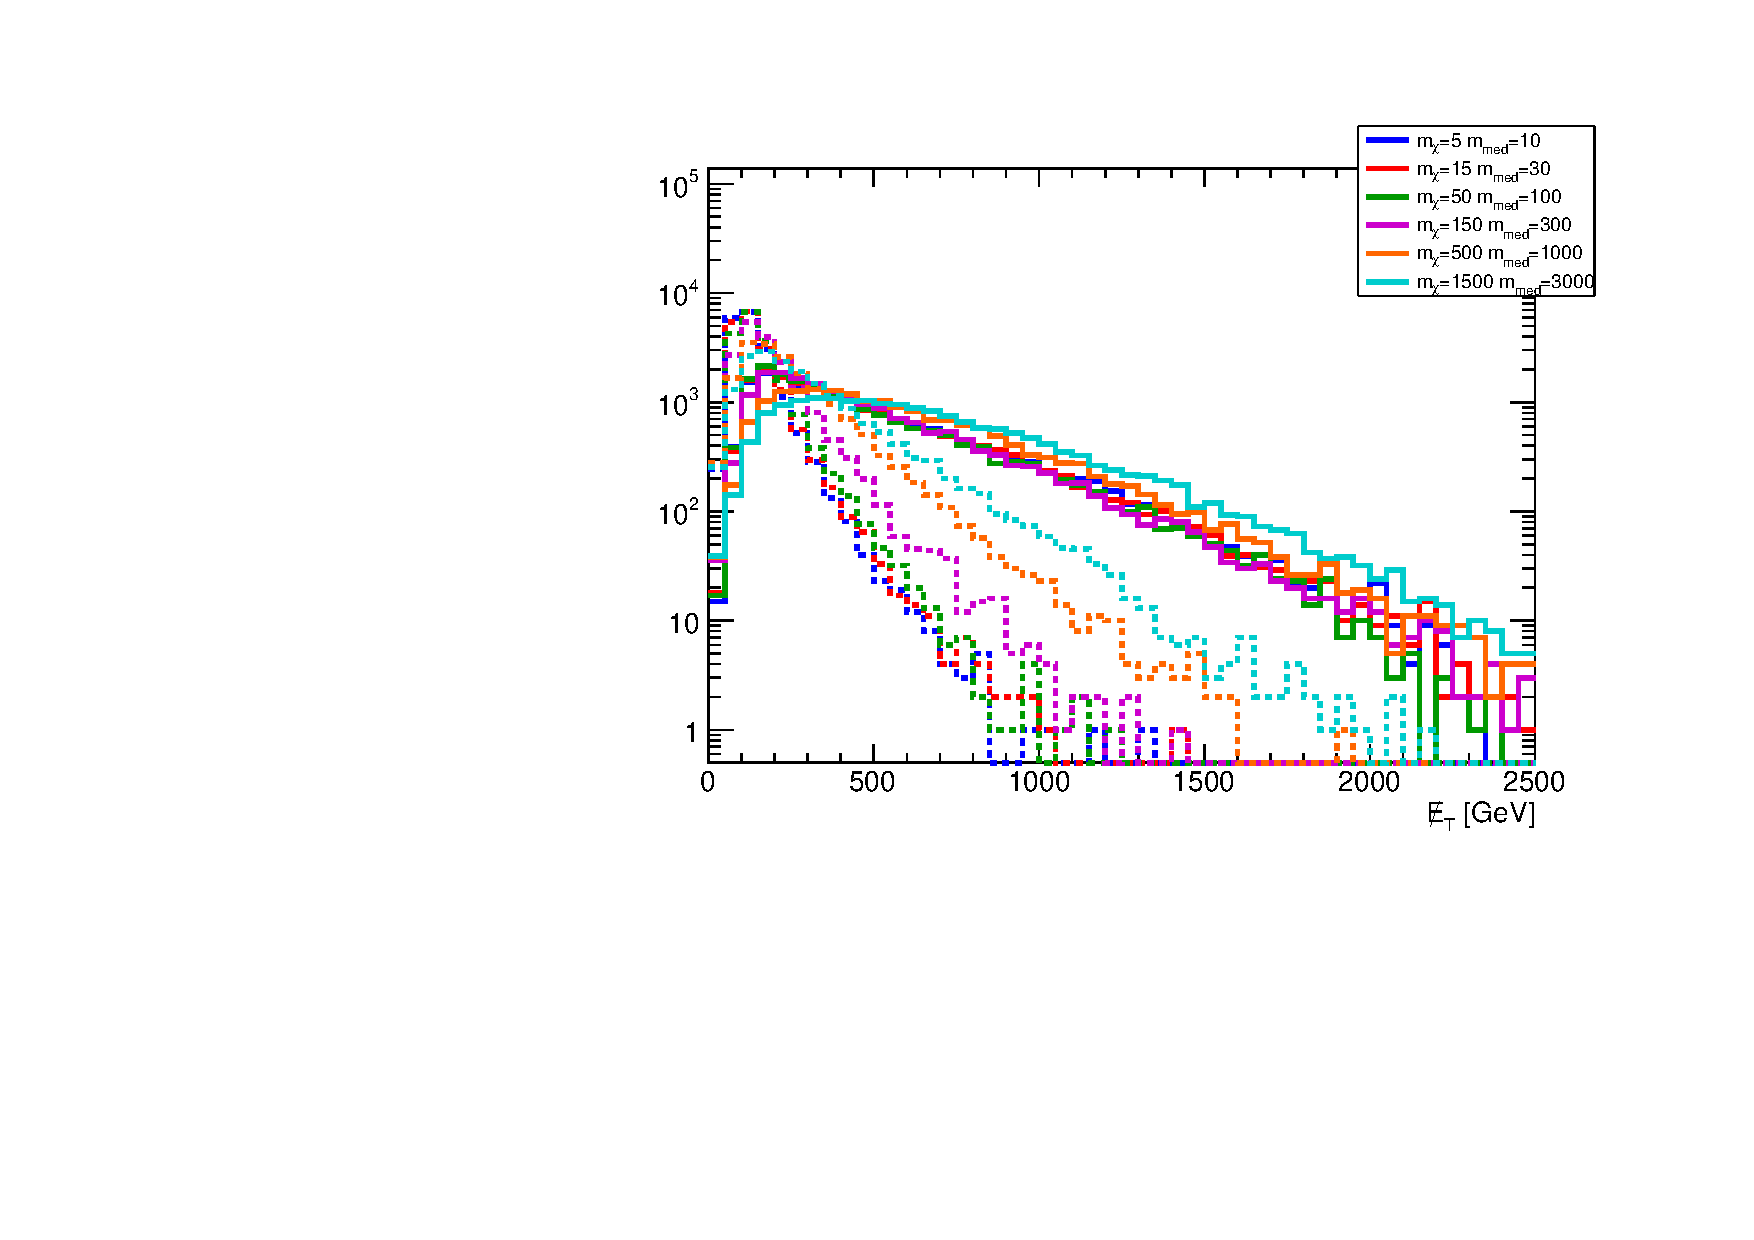
\includegraphics[width=0.5\textwidth]{figures/EW/monoWhad_Destructive/metPt}
}    
\caption{Kinematic distributions relevant for searches with W, Z and photons in the final state, 
for the simplified model
       with a vector mediator exchanged in the $s-$channel.}
\label{fig:DMV_EW_kinematics_SVMed}
\end{figure}

\subsection{Scalar mediator exchanged in the \schannel}
\label{sub:EW_Scalar}

The parameters for the model with a scalar mediator exchanged in the $s-$ channel 
follow those in Section~\ref{subsec:MonojetLikeModels}. 

Even though the sensitivity of mono-boson searches to this model is low and it may not
be in reach of early LHC searches, we recommend to generate this model for W, Z and photon searches 
in order to reproduce the kinematics of contact interaction operators described in Section~\ref{sub:EW_EFT_Dim5}, 
for later reinterpretation.  

\subsection{Colored scalar mediator exchanged in the \tchannel}

The model parameters with emission of an EW boson 
generally follow those in Section~\ref{subsec:MonojetLikeModels},
even though fewer diagrams are involved.   
A representative Feynman diagram can be
constructed by replacing a gluon in Fig.~\ref{fig:tchannelMonojet}
with a $\gamma,W,Z$ boson. See Ref.~\cite{Bell:2012rg} for a theoretical overview
of this model with specific examples for the Z+\MET final state. 

Figure~\ref{fig:TChan_EW_Zhad_MET} shows the \MET distribution for the hadronic Z+\MET final state, 
with varying dark matter and mediator mass, before any selection. 
The acceptance for a series of simplified analysis cuts 
(\MET$>$350~\gev, leading jet $p_T >$ 40~\gev, minimum azimuthal angle between jet and \MET > 0.4) 
applied at the generator level is shown in Figure~\ref{fig:TChan_EW_Zhad_acc}. 

\begin{figure}[h!]
\centering  
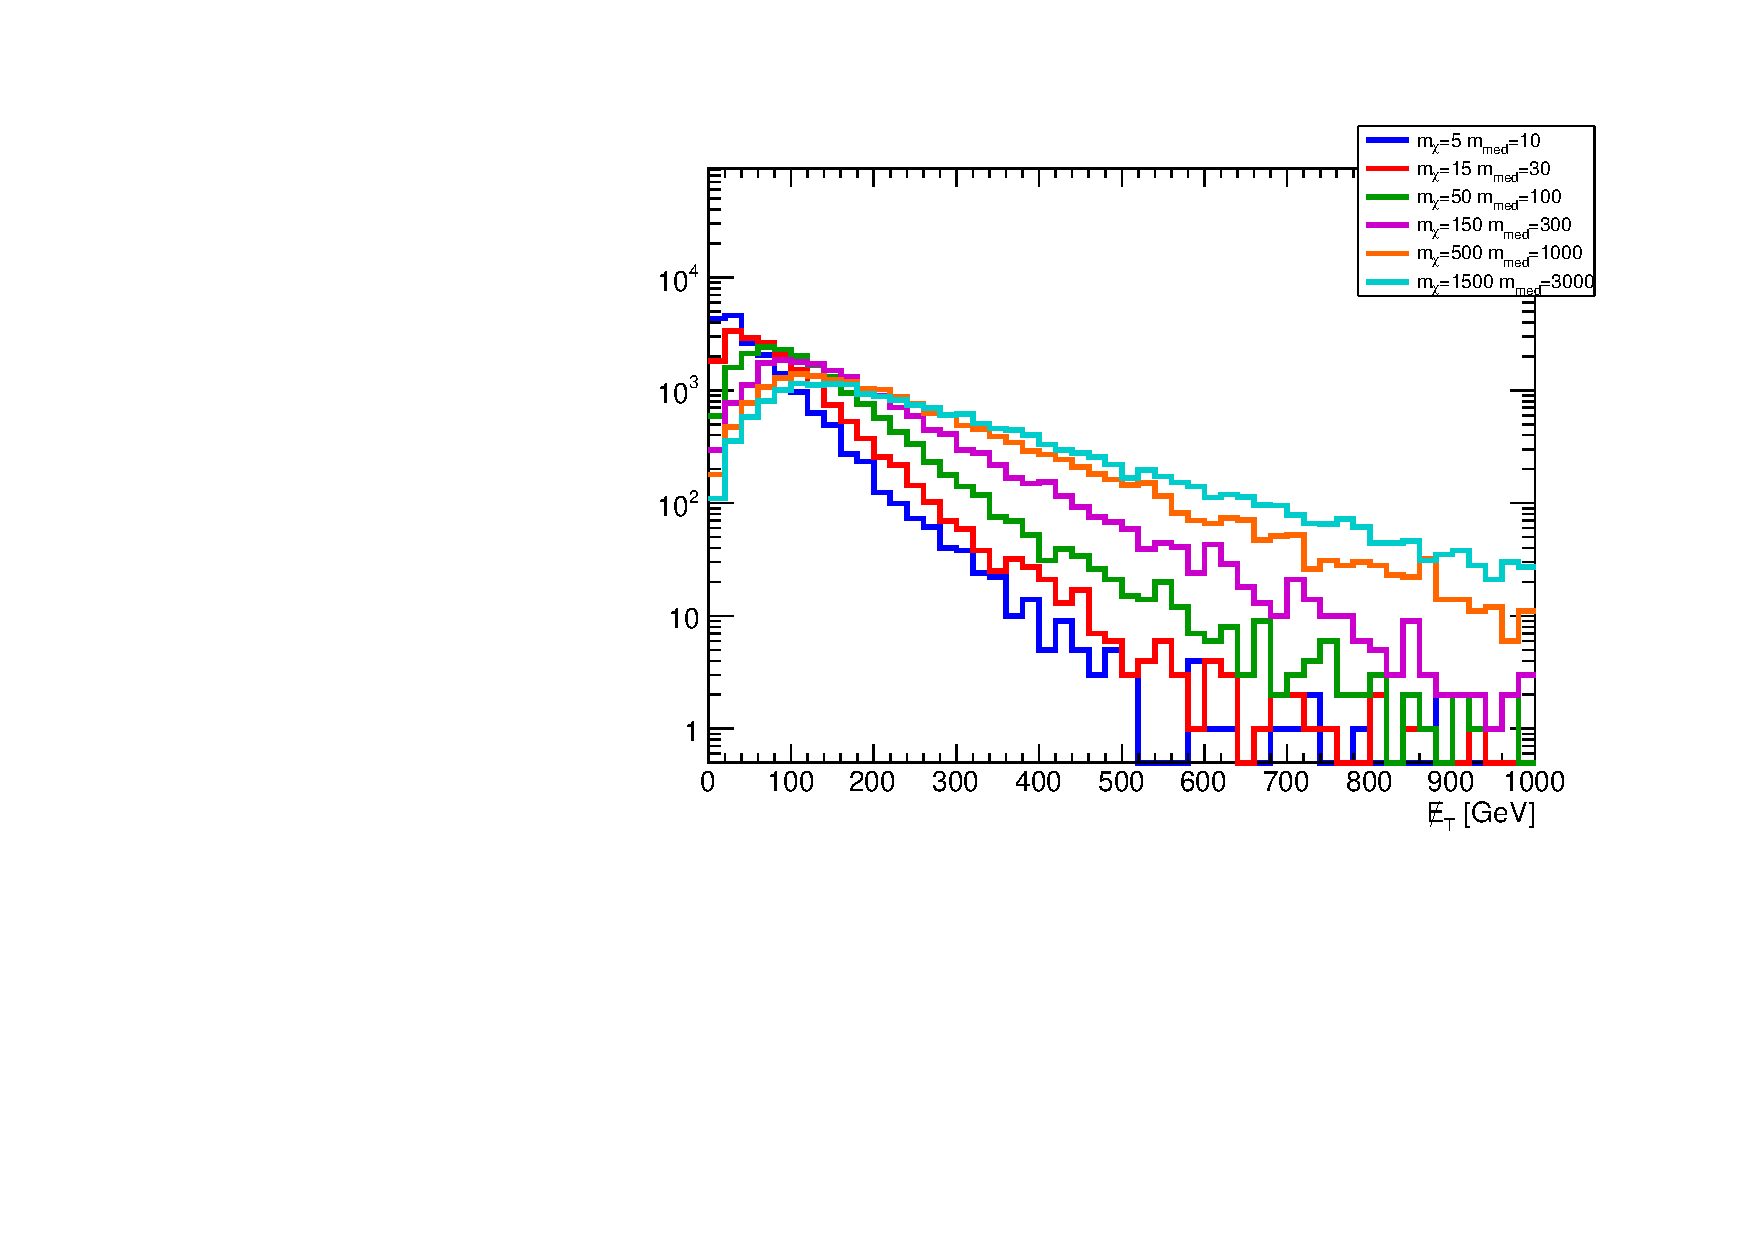
\includegraphics[width=0.8\textwidth]{figures/EW/monoZhad_TChannel/metPt}
\caption{Missing transverse momentum distribution for the hadronic Z+\MET final state,
for the simplified model with a colored scalar mediator exchanged in the $t-$channel.}
\label{fig:TChan_EW_Zhad_MET}
\end{figure}

\begin{figure}[h!]
\centering  
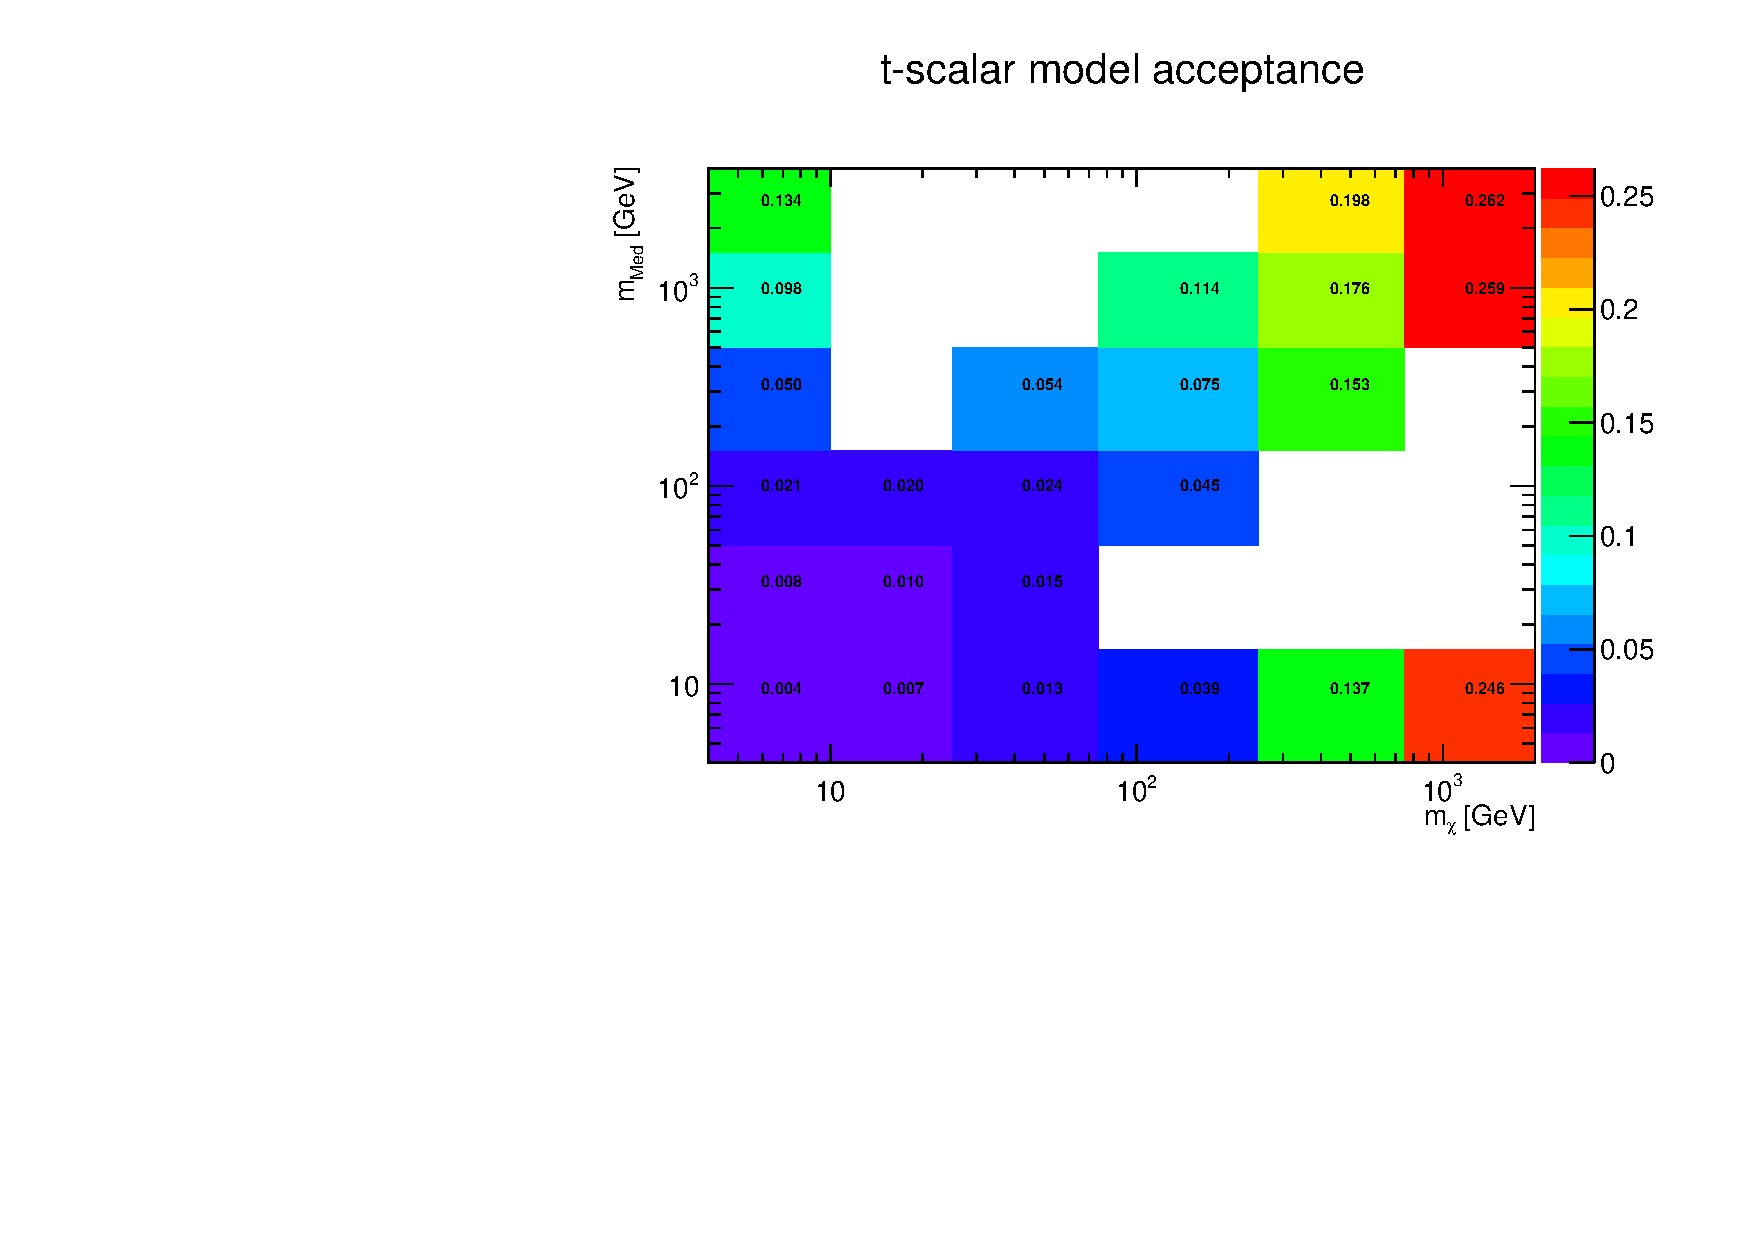
\includegraphics[width=0.8\textwidth]{figures/EW/monoZhad_TChannel/acc}
\caption{Acceptance table for the hadronic Z+\MET final state,
for the simplified model with a colored scalar mediator exchanged in the $t-$channel.}
\label{fig:TChan_EW_Zhad_acc}
\end{figure}

The parameter scan for the $t-$ channel model is still under discussion.~\Todo{The parameter scan, 
	and the conclusions that can be drawn from the plots below, need to be
	cross-checked with those in the monojet channel.}

\newthought{Model implementation discussed in the appendix}
%\subsection{Model implementation}
%
%These models are generated at leading
%order with MadGraph 2.2.2, using Pythia8 for the parton shower.
%Parameter cards can be found on the Forum SVN repository~\cite{ForumSVN_EW_DMV}.
%\Todo{Add models and instructions for other final states}.




\section{Specific simplified models including EW bosons, tailored to Higgs+MET searches}
%\svnidlong
%{$HeadURL: $}
%{$LastChangedDate: $}
%{$LastChangedRevision: $}
%{$LastChangedBy: $}
%\svnid{$Id: $}   

Three benchmark simplified models \cite{Carpenter:2013xra,Berlin:2014cfa} 
are recommended for Higgs+\MET searches:
\begin{itemize}
	\item A model where a vector mediator ($Z_B^\prime$) is exchanged in the \schannel, 
	radiates a Higgs boson, and decays into two DM particles (Fig.~\ref{fig:feyn_prod_monoH} (a)). As in Section \ref{sec:monojet_V}, we conservatively omit couplings of the $\Zprime_B$ to leptons.
    \item A model where a scalar mediator $S$ is emitted from the Higgs boson and decays to a pair of DM particles (Fig.~\ref{fig:feyn_prod_monoH_S}).
	\item A model where a vector \Zprime is produced resonantly and decays into a Higgs boson
	plus an intermediate heavy pseudoscalar particle $A^0$, in turn decaying into two DM particles (Fig. \ref{fig:feyn_prod_monoH} (b)). 
\end{itemize}


\begin{figure}[!htpb!tpd]
	\centering
	\unitlength=0.0046\textwidth
	\subfloat[\label{subfig:modelMonoHZprimeqq}]{
		\begin{feynmandiagram}[modelMonoHZprimeqq]
		\fmfleft{i1,i2}
		\fmfright{o1,o2,o3}
		\fmf{fermion}{i2,v1,i1}
		\fmflabel{\Large $q$}{i2}
		\fmflabel{\Large $\bar{q}$}{i1}
		\fmf{photon,label={\Large \Zprime}}{v1,v2}
		\fmf{photon,label={\Large \Zprime},label.angle=-100,label.distance=5}{v2,v3}
		\fmf{dashes}{v2,o3}
		\fmflabel{\Large $h$}{o3}
		% \fmfv{label={\Large $b,,\theta$},label.a=120,label.distance=5w}{v2}
		% \fmfv{label={\Large $y_{\chiDM}$},label.a=-45,label.distance=5w}{v3}
		\fmf{fermion}{o2,v3,o1}
		\fmflabel{\Large ${\bar{\chiDM}}$}{o1}
		\fmflabel{\Large ${\chiDM}$}{o2}
		\fmfdot{v1,v2,v3}
	\end{feynmandiagram}
	}
	%\\\vspace{\baselineskip}
	\subfloat[\label{subfig:modelMonoHSimplifiedA0}]{
	\begin{feynmandiagram}[modelMonoHSimplifiedA0]
		\fmfleft{i1,i2}
		\fmfright{o1,o2,o3}
		\fmf{fermion}{i2,v1,i1}
		\fmflabel{\Large $q$}{i2}
		\fmflabel{\Large $\bar{q}$}{i1}
		\fmf{photon,label={\Large \Zprime}}{v1,v2}
		\fmf{dashes}{v2,o3}
		\fmflabel{\Large $h$}{o3}
		\fmf{dots_arrow,label={\Large $A^0$},label.side=right}{v2,v3}
		\fmf{fermion,tension=2}{o2,v3,o1}
		\fmflabel{\Large ${\bar{\chiDM}}$}{o1}
		\fmflabel{\Large ${\chiDM}$}{o2}
		\fmfdot{v1}
	\end{feynmandiagram}
	}
	\caption
	{
		Examples of Feynman diagrams leading to Higgs+\MET events: 
                (a) %%% ref doesn't seem to work here
                a model with a vector mediator (\Zprime) 
		coupling with DM and with the Higgs boson $h$,
%\ref{subfig:modelMonoHZprimeqq}, %%% ref doesn't seem to work here
and
                (b) %%% ref doesn't seem to work here
		a 2HDM model with a new invisibly decaying pseudoscalar $A^0$ 
		from the decay of an on-shell resonance \Zprime giving rise to a Higgs+\MET signature
%~\ref{subfig:modelMonoHSimplifiedA0}
.
	}
	\label{fig:feyn_prod_monoH}
\end{figure}
		
\begin{figure}[!htpb!tpd]
	\centering
	\unitlength=0.0046\textwidth
	\subfloat[\label{subfig:modelMonoHbaryonicqq}]{
		\begin{feynmandiagram}[modelMonoHbaryonicqq]
			\fmfleft{i1,i2}
			\fmfright{o1,o2,o3}
			\fmf{fermion}{i2,v1,i1}
			\fmflabel{\Large $q$}{i2}
			\fmflabel{\Large $\bar{q}$}{i1}
			\fmf{dashes,label={\Large $h,,S$}}{v1,v2}
			\fmf{dashes,label={\Large $h,,S$},label.side=right}{v2,v3}
			\fmf{dashes}{v2,o3}
			\fmflabel{\Large $h$}{o3}
			\fmfv{label={$b,,\theta$},label.a=100,label.distance=3w}{v2}
			\fmfv{label={$y_{\chiDM}$},label.a=-45,label.distance=5w}{v3}
			\fmf{fermion}{o2,v3,o1}
			\fmflabel{\Large ${\bar{\chiDM}}$}{o1}
			\fmflabel{\Large ${\chiDM}$}{o2}
			\fmfdot{v1,v2,v3}
		\end{feynmandiagram}
	}\\\vspace{\baselineskip}
	\subfloat[\label{subfig:modelMonoHbaryonicgg}]{
		\begin{feynmandiagram}[modelMonoHbaryonicgg]
			\fmfleft{i1,i2}
			\fmfright{o1,o2,o3}
			\fmf{gluon}{i1,vt1}
			\fmf{gluon}{i2,vt2}
			\fmflabel{\Large $g$}{i2}
			\fmflabel{\Large $g$}{i1}
			\fmf{fermion,label={\Large $t$}}{vt1,vt2}
			\fmf{fermion}{vt2,v1,vt1}
			\fmf{dashes,label={\Large $h,,S$},label.side=right}{v1,v2}
			\fmf{dashes,label={\Large $h,,S$},label.side=right,label.d=5}{v2,v3}
			\fmf{dashes}{v2,o3}
			\fmflabel{\Large $h$}{o3}
			\fmfv{label={$b,,\theta$},label.a=120,label.distance=3w}{v2}
			\fmfv{label={$y_{\chiDM}$},label.a=-45,label.distance=5w}{v3}
			\fmf{fermion}{o2,v3,o1}
			\fmflabel{\Large ${\bar{\chiDM}}$}{o1}
			\fmflabel{\Large ${\chiDM}$}{o2}
			\fmfdot{v1,v2,v3}
		\end{feynmandiagram}
	}
	\subfloat[\label{subfig:modelMonoHbaryonicggS}]{
	\begin{feynmandiagram}[modelMonoHbaryonicggS]
		\fmfleft{i1,i2}
		\fmfright{o1,o2,o3}
		\fmf{gluon}{i1,vt1}
		\fmf{gluon}{i2,vt2}
		\fmflabel{\Large $g$}{i2}
		\fmflabel{\Large $g$}{i1}
		\fmf{fermion,label={\Large $t$}}{vt1,vt2}
		\fmf{fermion}{vt2,v2,v1,vt1}
		\fmf{dashes}{v2,o3}
		\fmflabel{\Large $h$}{o3}
		\fmf{dashes,label={\Large $h,,S$},label.side=right,label.d=5}{v1,v3}
		\fmfv{label={$y_{\chiDM}$},label.a=-45,label.distance=5w}{v3}
		\fmf{fermion}{o2,v3,o1}
		\fmflabel{\Large ${\bar{\chiDM}}$}{o1}
		\fmflabel{\Large ${\chiDM}$}{o2}
		\fmfdot{v1,v2,v3,vt1,vt2}
	\end{feynmandiagram}

	}
	\caption
	{
		Examples of Feynman diagrams leading to Higgs+\MET events for a model with a scalar mediator ($S$) 
		coupling with DM and with the Higgs boson $h$. 
	}
	\label{fig:feyn_prod_monoH_S}
\end{figure}

These models are kinematically distinct from one another, as shown in the comparison of the 
\MET spectra in Fig.~\ref{fig:METSimpMonoHiggs} for high and low masses of the pseudoscalar mediator. 
Figure~\ref{fig:METSimpMonoHiggs} (a) shows the \MET distribution 
for models with high mediator masses ($m_{S} = 1$~\tev, $m_{\Zprime} = 1$~\tev, $m_{A^0} = 1$~\tev)
and DM mass of either 50 ($Z_B'$ and $A^0$ models) or 65~\gev (scalar mediator model).
Figure~\ref{fig:METSimpMonoHiggs} (b)  shows the \MET distribution 
for models with low pseudoscalar mediator masses ($m_{Z_B'} = 100$~\gev, $m_{\Zprime} = 1$~\tev, $m_{A^0} = 100$~\gev)
and DM mass of 1~\tev for all models. 

\begin{figure}[hbpt!]
	\centering
	\subfloat[High mediator mass]{
		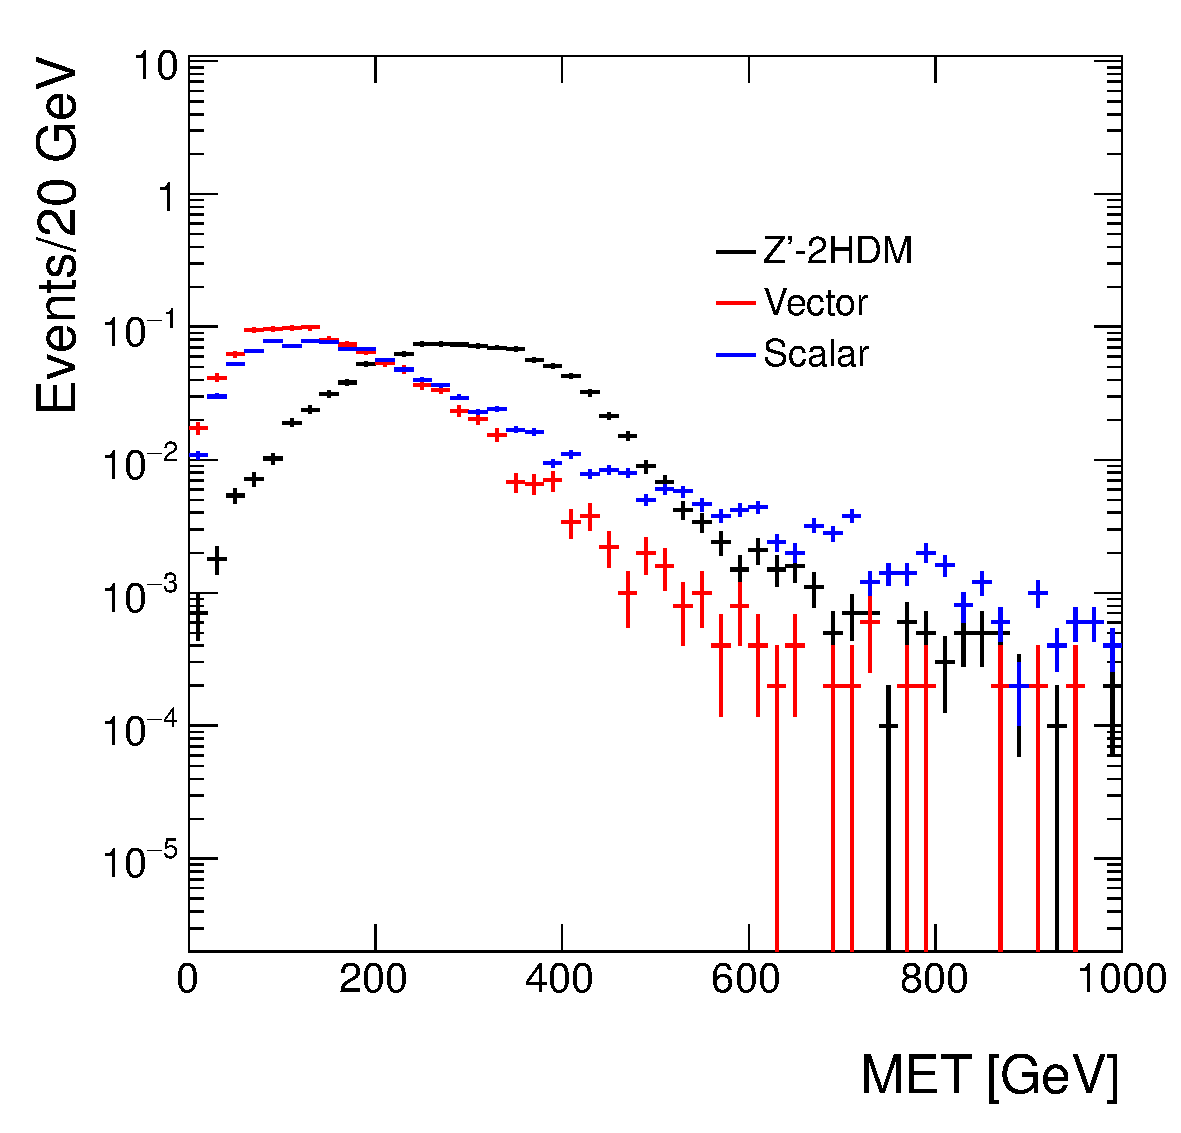
\includegraphics[width=0.75\linewidth]{figures/EW/monoH/models_cmp_MET_et_Log} \label{fig:met_cmp_high}
	}\\
	\subfloat[Low mediator mass]{
		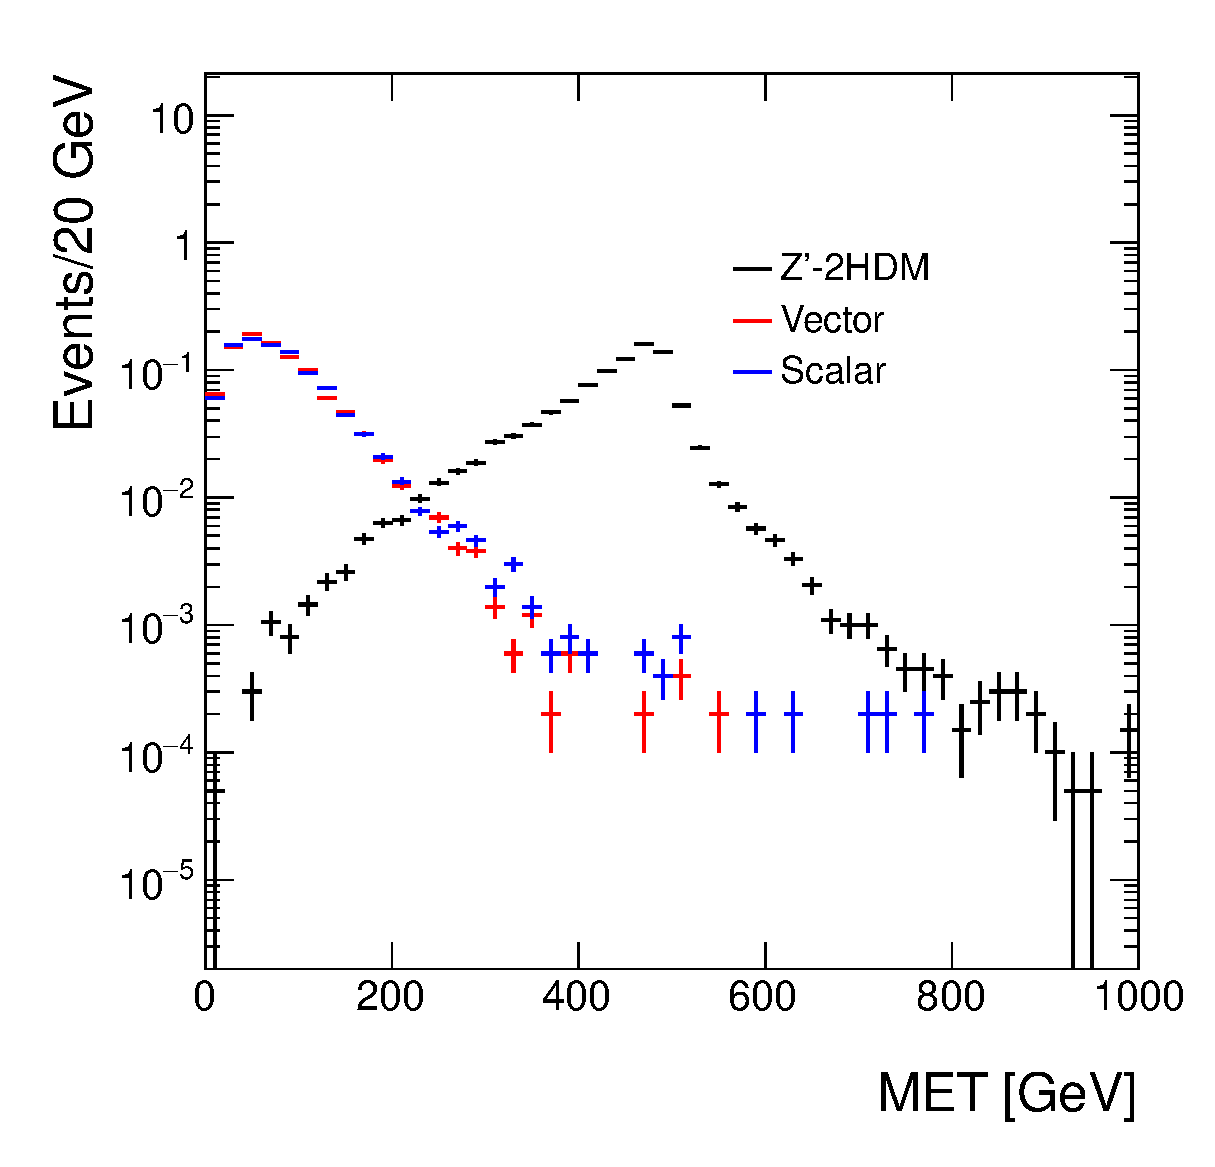
\includegraphics[width=0.75\linewidth]{figures/EW/monoH/models_cmp_low_MET_et_Log} \label{fig:met_cmp_low}
	}
	\caption{Comparison of the missing transverse momentum distributions at generator level in different 
		simplified models leading to a Higgs+\MET signature. The model parameter settings are detailed in the text. The figures in this Section have been obtained using LO UFO models within \madgraph v2.2.3, interfaced to \pythia 8 for the parton shower.  		
		\label{fig:METSimpMonoHiggs}}
\end{figure}

Predictions for this class of models have been so far considered at LO+PS, even though they could be extended to NLO+PS in the near future. The studies in this Section
have been performed using a model within \madgraph v2.2.3, interfaced to \pythia 8 for the parton shower.  
The implementation details for these models are discussed in Section~\ref{sec:monoHImplementation}.

\subsection{\MET+Higgs from a baryonic \Zprime}

The model shown in Fig.~\ref{fig:feyn_prod_monoH} (a)
postulates a new gauge boson \Zprime corresponding to a new $U(1)_B$ baryon 
number symmetry. The stable baryonic states included in this model are the DM candidate particles.
The mass of the \Zprime boson is acquired through a baryonic Higgs $h_B$, which mixes with the 
SM Higgs boson. 

The interactions between the \Zprime, the quarks and the DM are described by 
the following Lagrangian:   

\be \label{ZprimeDM}
%%\mathscr{
	\mathcal{L} =  \gq  \bar q \gamma^\mu q  Z_\mu' +
%
%\left\{ \begin{array}{cc}
%	%i  \gDM  \chiDM^\dagger \smash{ \overset{\leftrightarrow}{\partial^\mu}}  \chiDM  \Zprime_\mu + \gDM^2 |\chiDM|^2 \Zprime_\mu Z^{\prime\mu} & {\rm scalar}  
	 \gDM  \bar\chiDM \gamma^\mu \chiDM Z_\mu' .
\ee

The quark couplings \gq are fixed to be equal to one third of the gauge coupling $g_B$, 
while the DM coupling to the \Zprime are proportional to the baryon number and to the gauge coupling 
($g_{\chiDM} = B g_B$). No leptonic couplings of the \Zprime are allowed, thus evading dilepton constraints. 
After incorporating the mixing of the baryonic and SM Higgs bosons, this model is 
is described by the following Lagrangian term at energies below $m_{\Zprime}$~\footnote{The operator 
	in Eqn.~\ref{U1Beft} is an effective one, to highlight the two main terms. The full dimension-4 simplified
	model is used in the model for event generation.}: 

\be \label{U1Beft}
 \mathcal{L}_{\rm eff} = - \frac{\gq \gDM }{m_{\Zprime}^2} \bar{q} \gamma^\mu q \bar\chiDM \gamma_\mu \chiDM \Big( 1 + \frac{g_{h \Zprime \Zprime} }{m_{\Zprime}^2} h \Big) \, ,
\ee

The first term of this equation
is the standard \modelDMV model in the large $M_{Z^\prime}$ limit.  This term can lead
to a monojet signature, which can be also used to constrain this model.
The second term describes the interaction between the \Zprime and the SM Higgs boson,
via the coupling $g_{h \Zprime \Zprime} = \frac{m_{\Zprime}2 \sin\theta}{v_B}$, where
$\sin\theta$ is the mixing angle between the SM Higgs and the baryonic Higgs $h_B$, and $v_B$ is the
Baryonic Higgs vacuum expectation value. 

%In its most general form, this model can lead to mono-Z signals as well. However, in this case
%there is no $Z-Z'$ mixing from the $h \Zprime \Zprime$ term, since this term arises only
%after $U(1)_B$ is broken. A mixing angle can come from terms involving 
%the field strengths of $Z$ and $Z'$: this is a free parameter, that is set to be small
%in the model considered for mono-Higgs signatures. 

In its most general form, this model can contribute to mono-Z signals due to the \Zprime mixing with the Z or photon. Note that EWSB and $ U(1)_B $ breaking do not lead to this mixing at tree-level. Instead, kinetic mixing occurs between the $ U(1)_Y $ and $ U(1)_B $ gauge bosons due to the gauge invariant term $ F^{\mu\nu}_Y F_{B\mu\nu} $. This mixing is a free parameter which we assume to be small in order to focus on the mono-Higgs signature. Mixing may also occur due to radiative corrections, however this is model dependent so we choose to ignore this here.

%Left for later
%	1- Mention sensitivity difference wrt monojet? 
%	2- Mention why we don't consider the dark Z model?]}

The predictions of the model depend upon the two additional
parameters beyond an \schannel simplified model, namely the
mixing angle between baryonic Higgs $h_B$ and the SM-like Higgs boson $\sin\theta$ and the coupling of the mediator to SM-like Higgs boson, $g_{h\Zprime \Zprime}$.
Thus, a full model is specified by:

\be
\left\{\mMed ,\, \mDM ,\, \gDM ,\, \gq ,\, \sin\theta ,\, g_{h\Zprime \Zprime}\right\}.
\ee

\subsubsection{Parameter scan} 

The width of the \Zprime mediator is calculated using all possible decays to SM particles (quarks) and to pairs of DM particles if kinematically allowed
as in the \modelDMV model.

The dependence of the missing transverse momentum (\MET) on the model parameters 
is studied by varying the parameters one at a time. The variation of parameters 
other than \mMed and \mDM does not result in significant 
variations of the \MET spectrum, as shown in Figures~\ref{fig:metVectorCoupling}. 
Figure~\ref{fig:metVectorMass} shows that for an on-shell mediator, 
varying \mDM with the other parameters fixed does not affect the \MET distribution, while 
the distribution broadens significantly in the case of an off-shell mediator. 
For this reason, the same grid in \mmed, \mdm as for the vector mediator
of the jet+\MET search (Table~\ref{tab:mDMmMedScan_VA}) is chosen as a starting point. 
The coupling $g_{h\Zprime \Zprime}$, along with \gq and \gDM, are subject to perturbativity bounds:

$$\gq, \gDM < 4\pi $$
and

$$  g_{h \Zprime \Zprime} < \sqrt{4\pi}m_{\Zprime}\sin\theta$$ 
The value $g_{h \Zprime \Zprime}/m_{\Zprime} = 1$ is chosen as a benchmark value for the generation 
of Monte Carlo samples since it maximizes the cross section (as shown in the following paragraph)
without violating the bounds. The mediator-DM coupling \gDM is fixed to 1, and  
the mediator-quark $g_{q}$ coupling is fixed to 1/3. 
The kinematic distributions do not change as a function of these parameters, so 
results for other values of  $g_{h \Zprime \Zprime}/m_{\Zprime}$, \gDM and \gq can be 
obtained through rescaling by the appropriate cross sections. 

Figs~\ref{fig:VectorHbb_100} and ~\ref{fig:VectorHbb_1000} show the kinematic distributions for the two leading jets
in the $H \to \bar b b$ decay channel, for two values of the mediator mass and varying the DM mass.  

Analyses should perform further studies, beyond those studies performed for the forum, 
to estimate the reach of the analysis with respect to all points in the grid and therefore decide 
on a smaller set of grid points to be generated.

\begin{figure}[htpb!]
	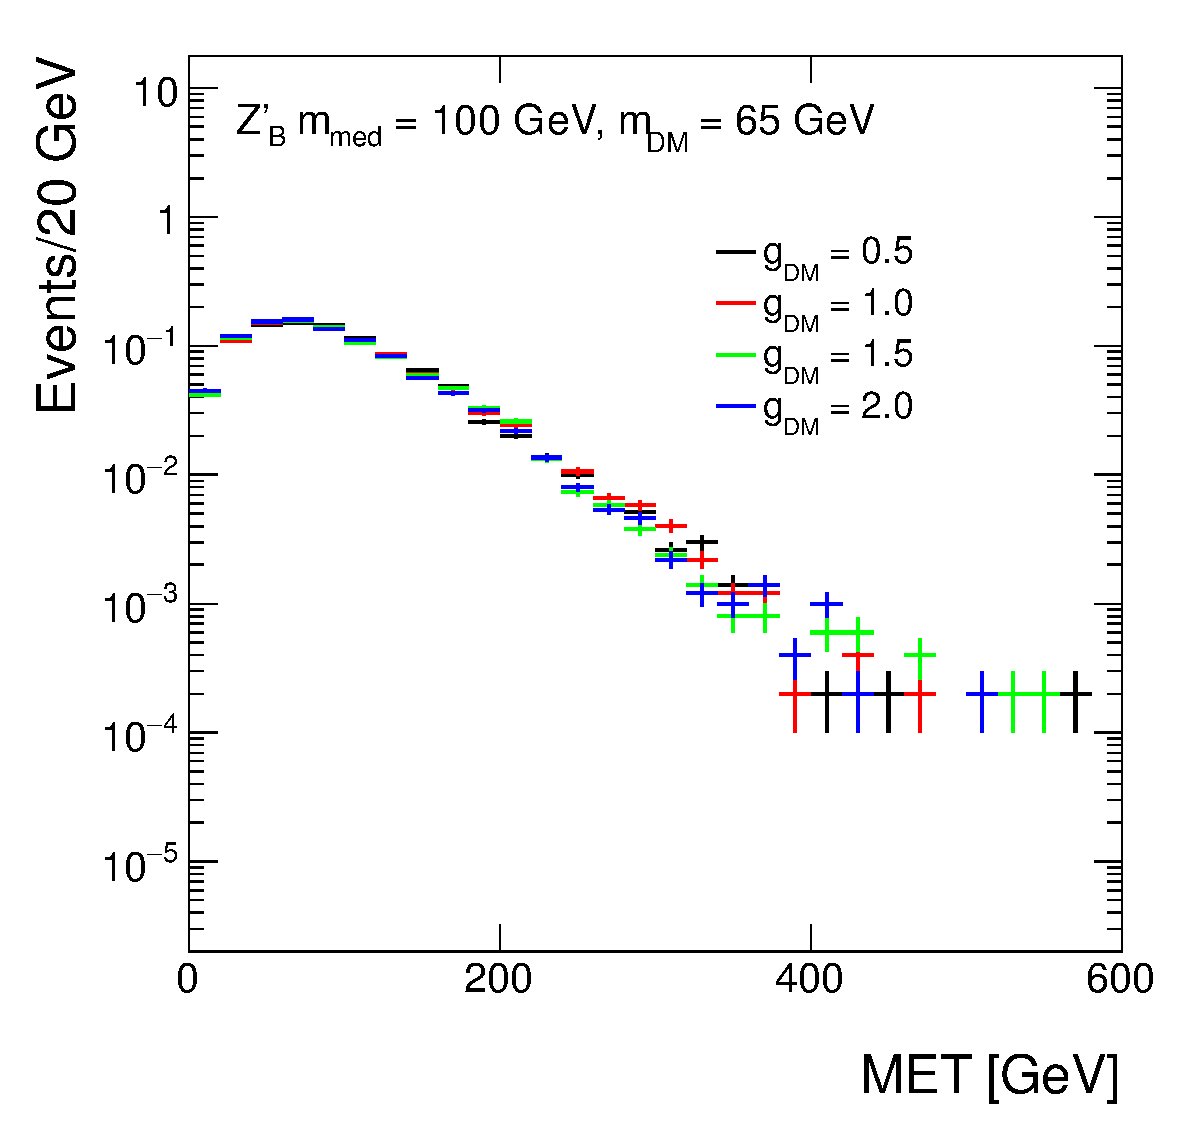
\includegraphics[width=0.75\linewidth]{figures/EW/monoH/z_gdm_MET_et_Log}\\
	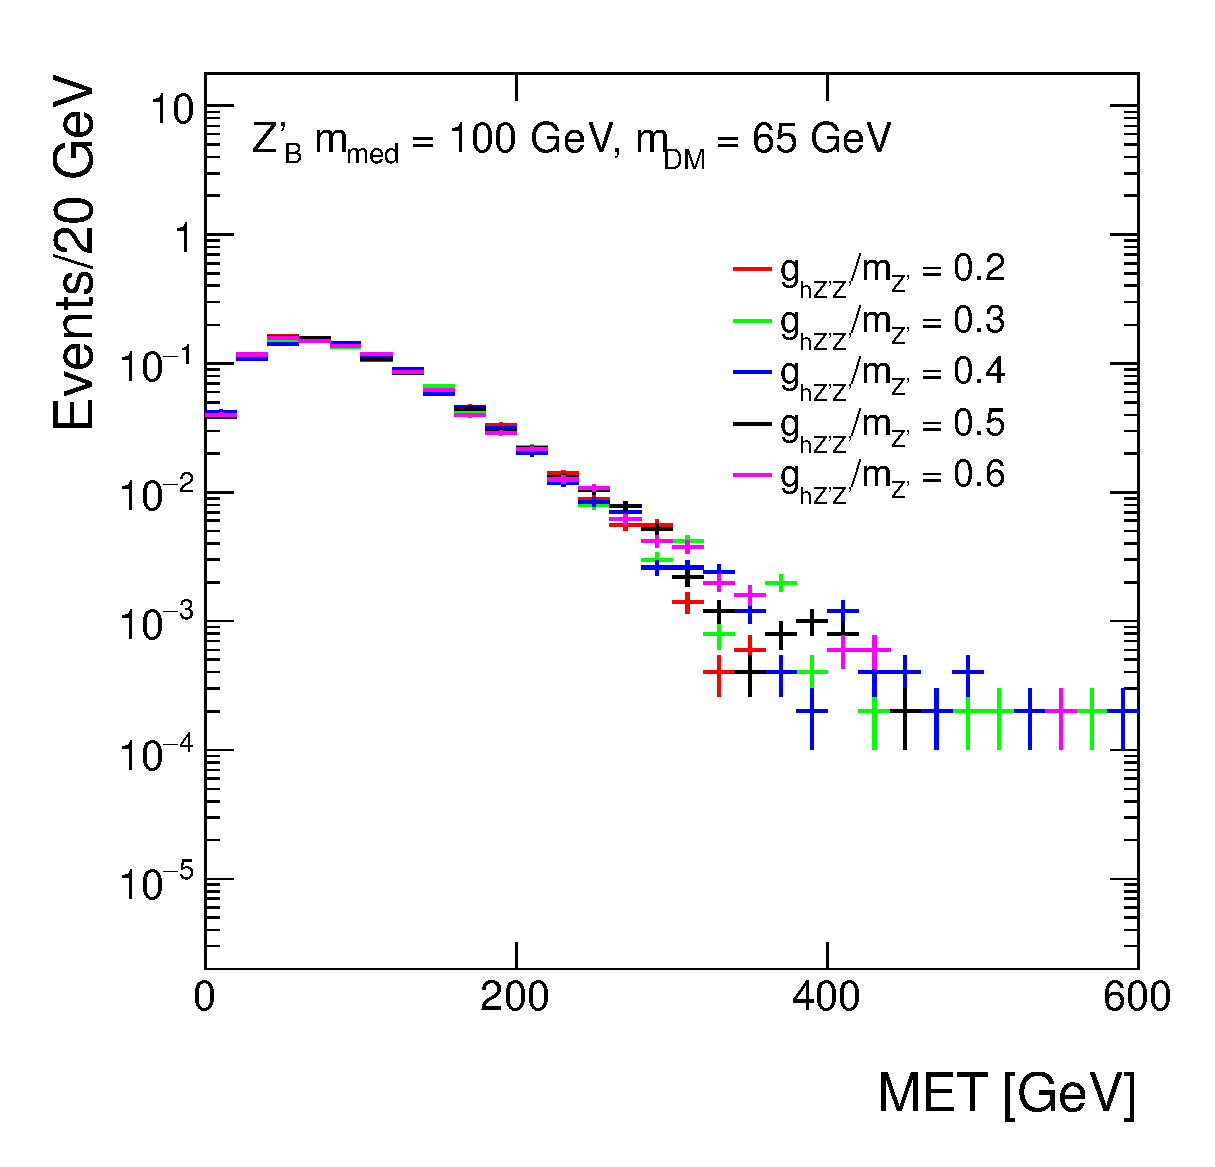
\includegraphics[width=0.75\linewidth]{figures/EW/monoH/z_ratio_MET_et_Log}
	\caption{Missing transverse momentum distributions at generator level in the vector 
		mediator scenario for different values of: the mediator-dark matter coupling \gDM (left),
		and the coupling between the mediator and the SM-like Higgs boson, scaled by the mediator mass, 
		$g_{h \Zprime \Zprime}/m_{\Zprime}$ (right).
		\label{fig:metVectorCoupling}}
\end{figure}

\begin{figure}[htpb!]
	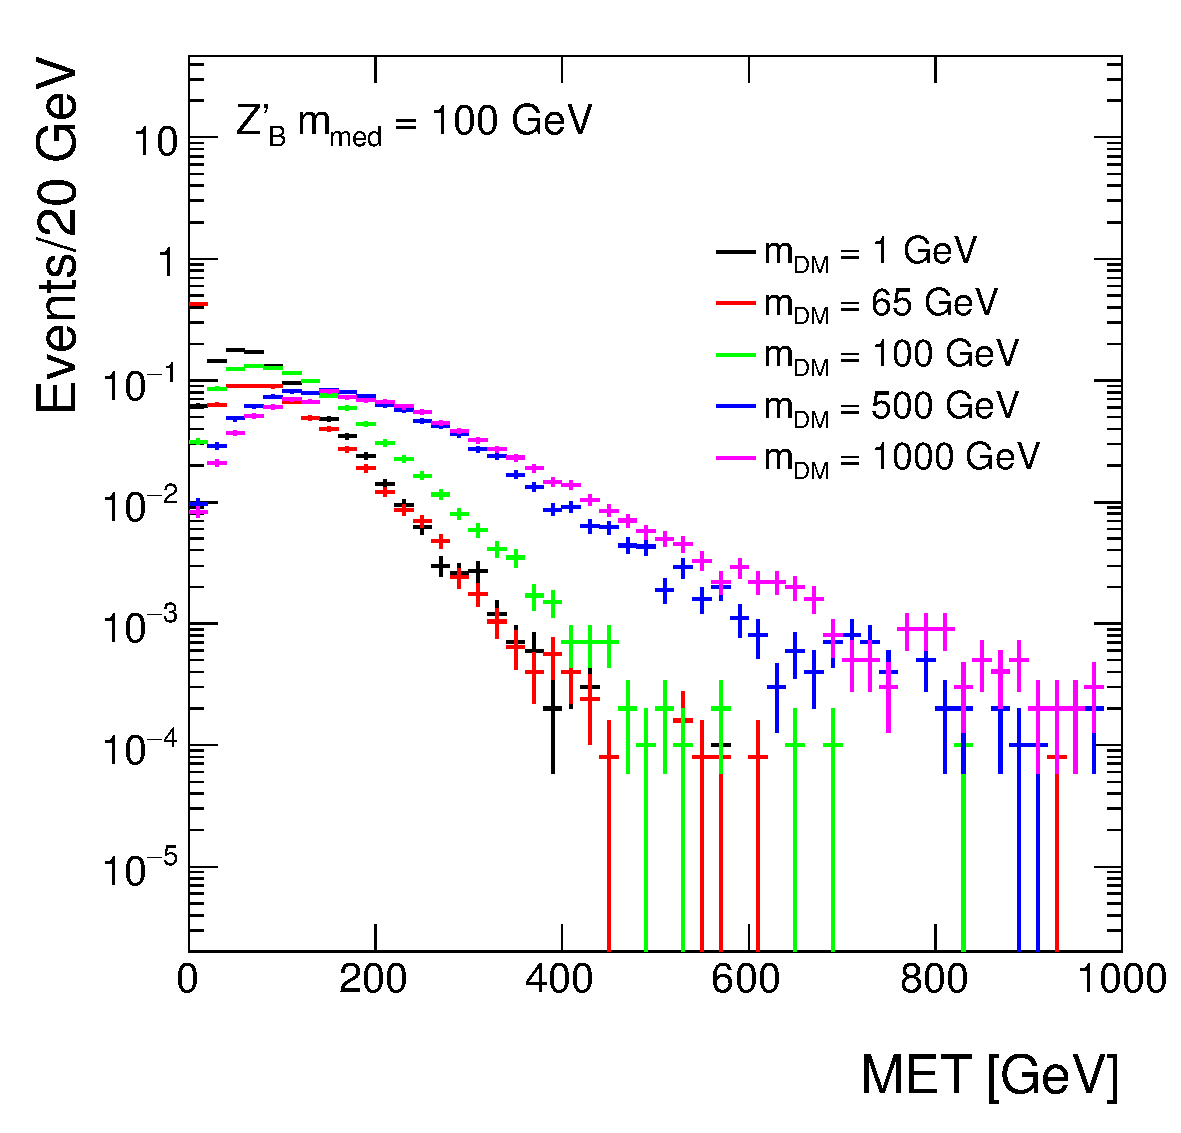
\includegraphics[width=0.75\linewidth]{figures/EW/monoH/zprime_100_MET_et_Log}\\
	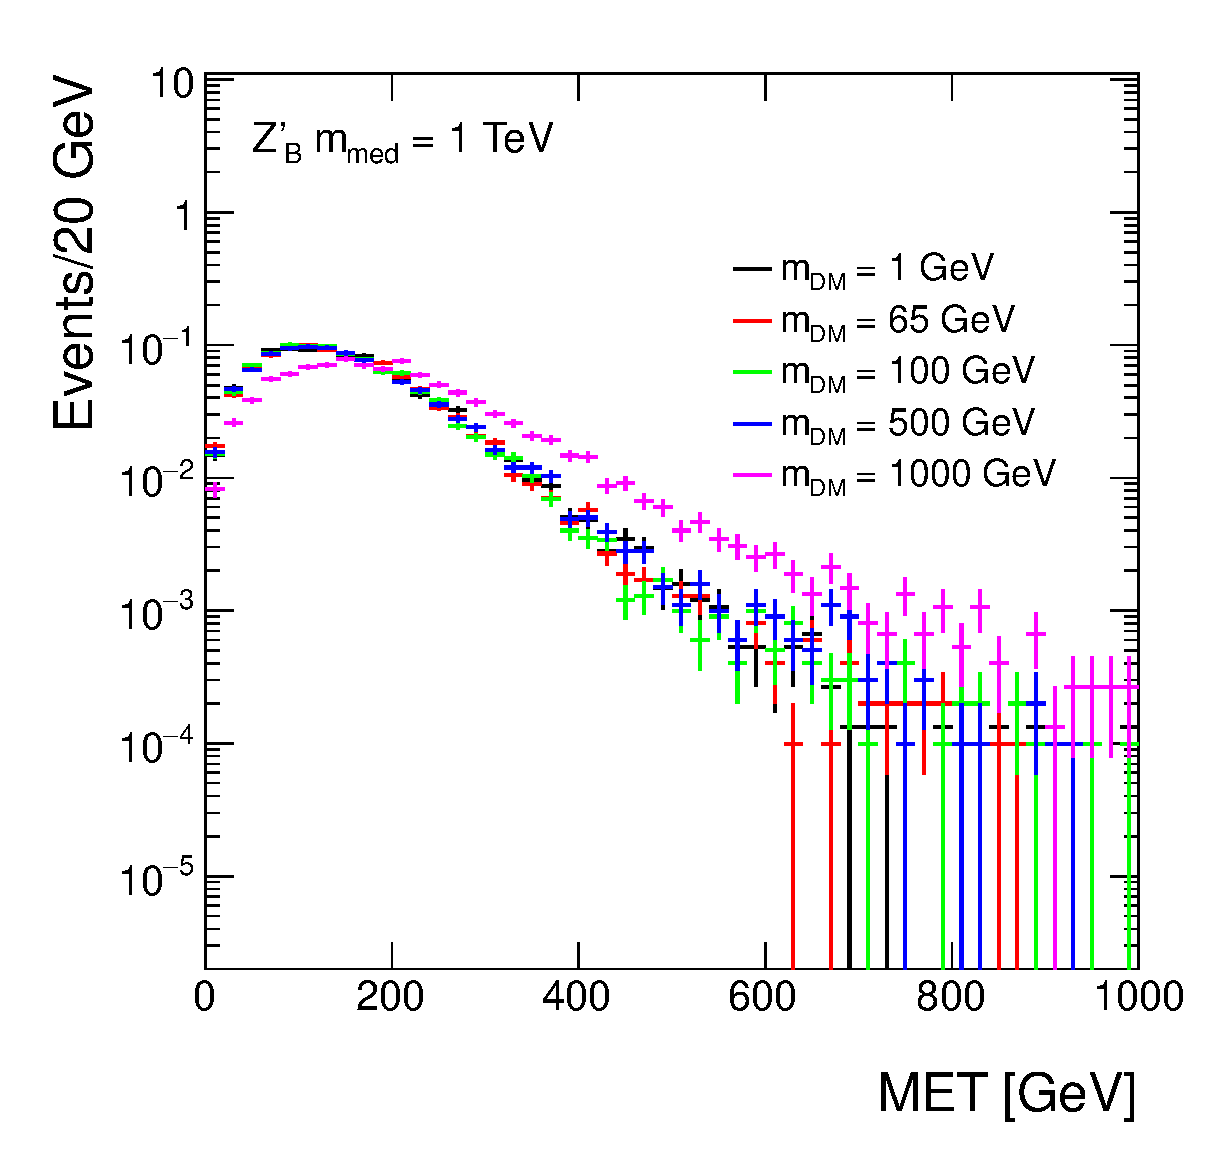
\includegraphics[width=0.75\linewidth]{figures/EW/monoH/zprime_1000_MET_et_Log}
	\caption{Missing transverse momentum distributions at generator level in the vector 
		mediator scenario: for different values of the dark matter mass \mDM 
		and a mediator mass of \mmed = 100~\gev (left) and \mmed = 1~\tev (right).
		\label{fig:metVectorMass} }
\end{figure}


\begin{figure}[htpb!]
	\centering
	\subfloat[Leading $b-$jet transverse momentum]{
		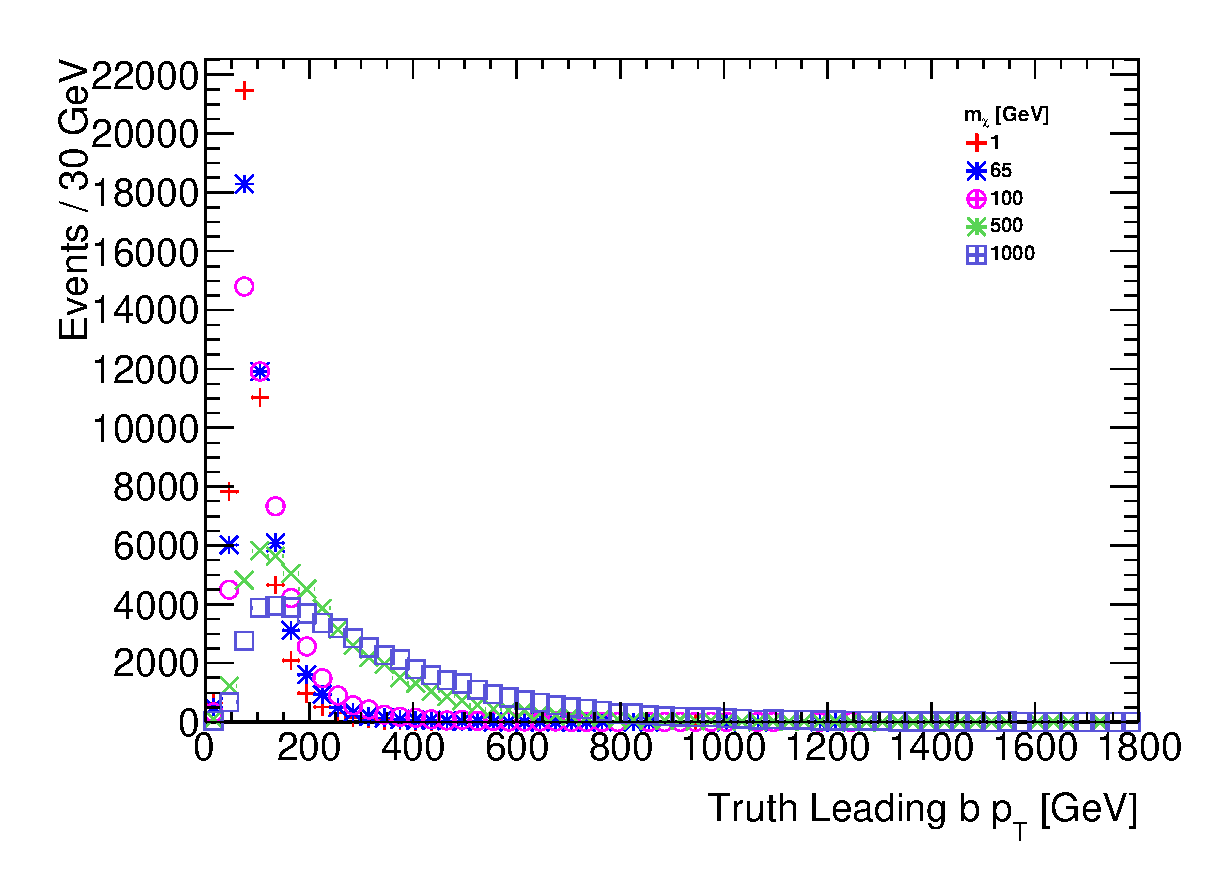
\includegraphics[width=0.75\linewidth]{figures/EW/monoH/zpzp100/truth_leading_b_pt} %\label{fig:met_cmp_high}
	}\hfill
	\subfloat[Leading $b-$jet pseudorapidity]{
		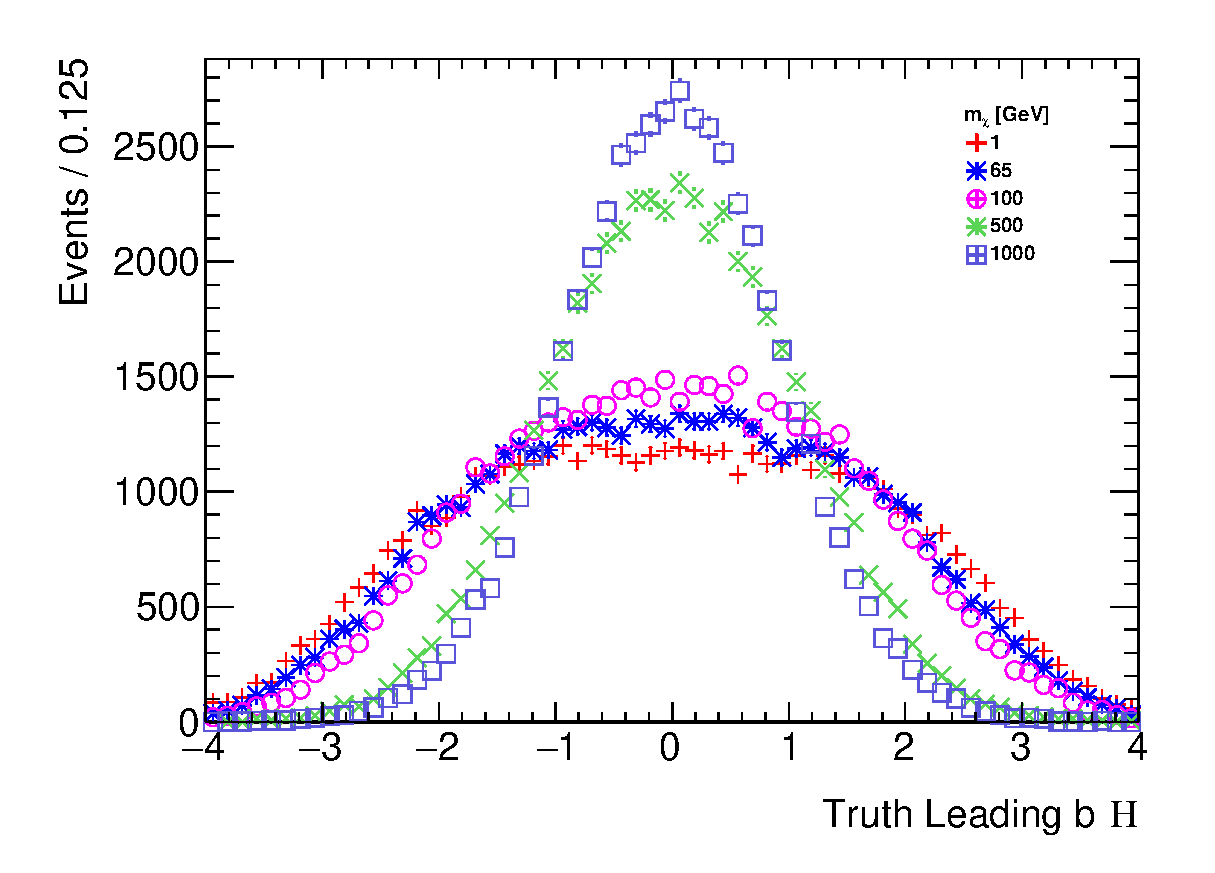
\includegraphics[width=0.75\linewidth]{figures/EW/monoH/zpzp100/truth_leading_b_eta} %\label{fig:met_cmp_low}
	}\hfill
	\subfloat[Angular distance between the two leading $b-$jets]{
		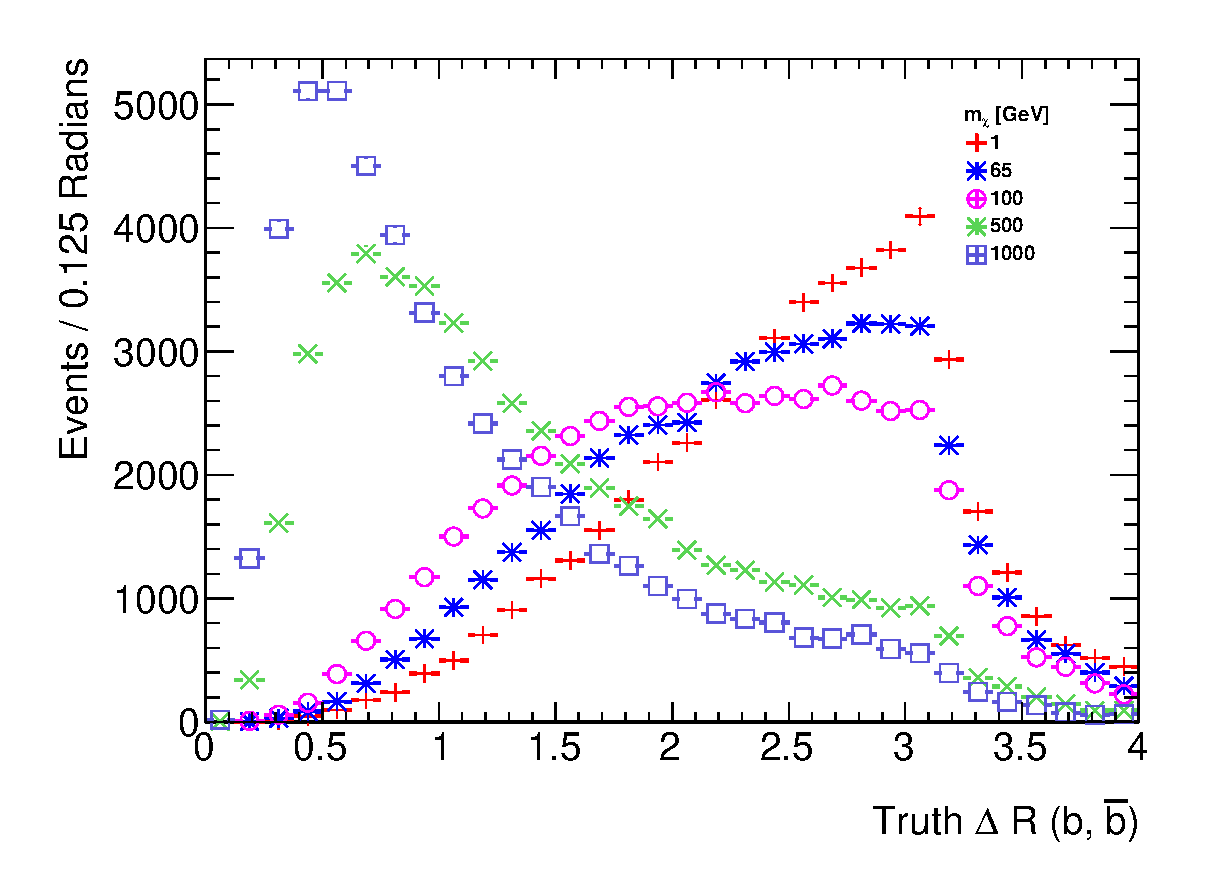
\includegraphics[width=0.75\linewidth]{figures/EW/monoH/zpzp100/truth_bb_deltar} %\label{fig:met_cmp_low}
	}
	\caption{Comparison of the kinematic distributions for the two leading $b-$jets (from the Higgs decay) in the vector \Zprime simplified model, 
		when fixing the \Zprime mass to 100~\gev and varying the DM mass. 
		\label{fig:VectorHbb_100}}
\end{figure}

%	\hfill
%	\subfloat[Leading $b-$jet transverse momentum]{
%		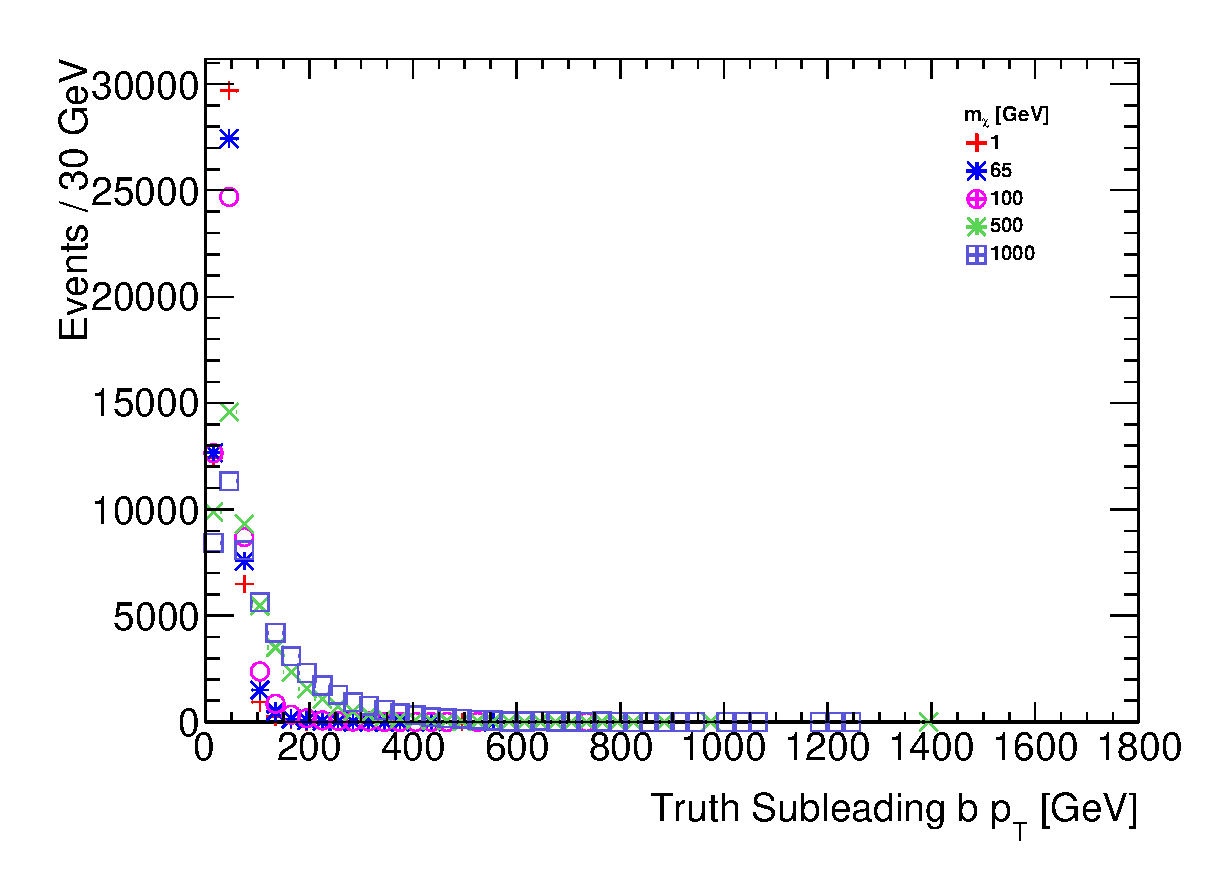
\includegraphics[width=0.95\linewidth]{figures/EW/monoH/zpzp100/truth_subleading_b_pt} %\label{fig:met_cmp_high}
%	}
%	\hfill
%	\subfloat[Leading $b-$jet pseudorapidity]{
%		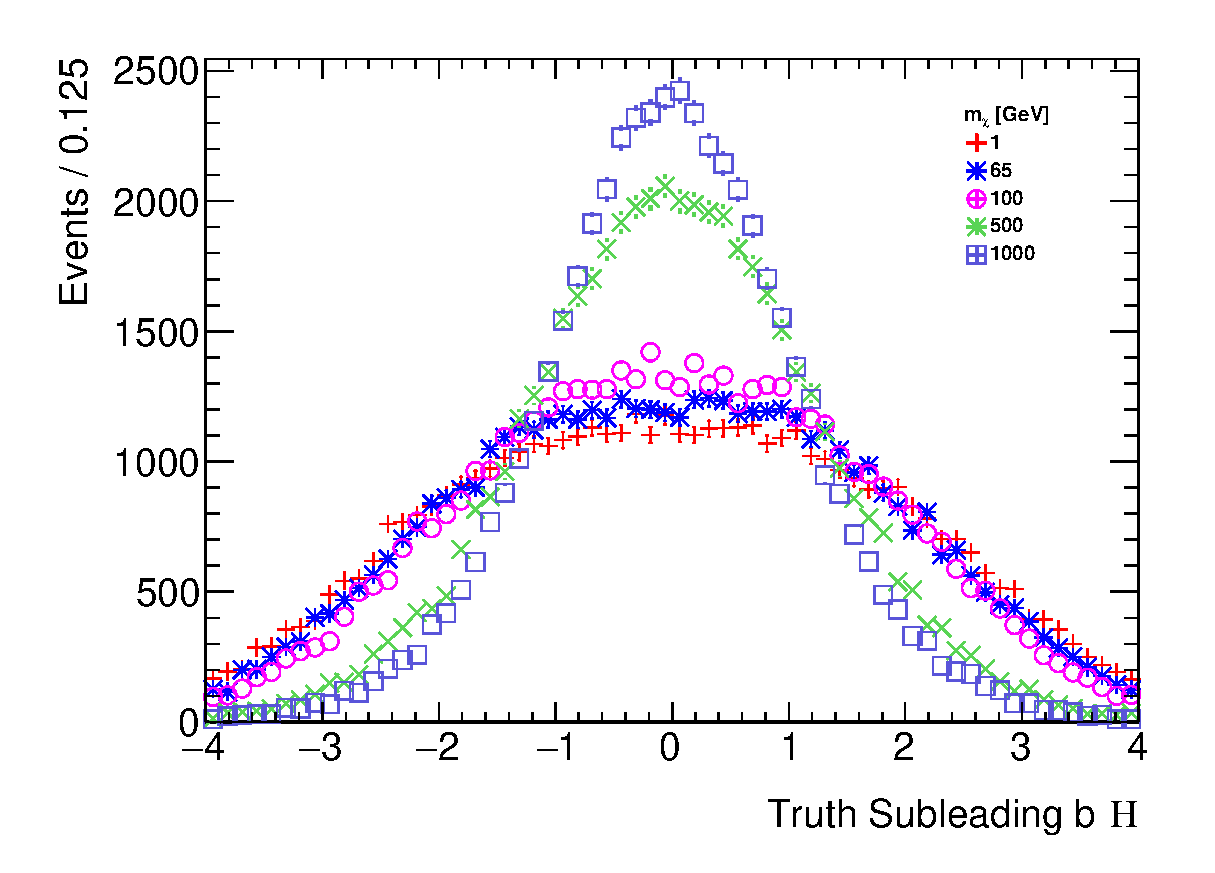
\includegraphics[width=0.95\linewidth]{figures/EW/monoH/zpzp100/truth_subleading_b_eta} %\label{fig:met_cmp_low}
%	}

\begin{figure}[htpb!]
	\centering
	\subfloat[Leading $b-$jet transverse momentum]{
		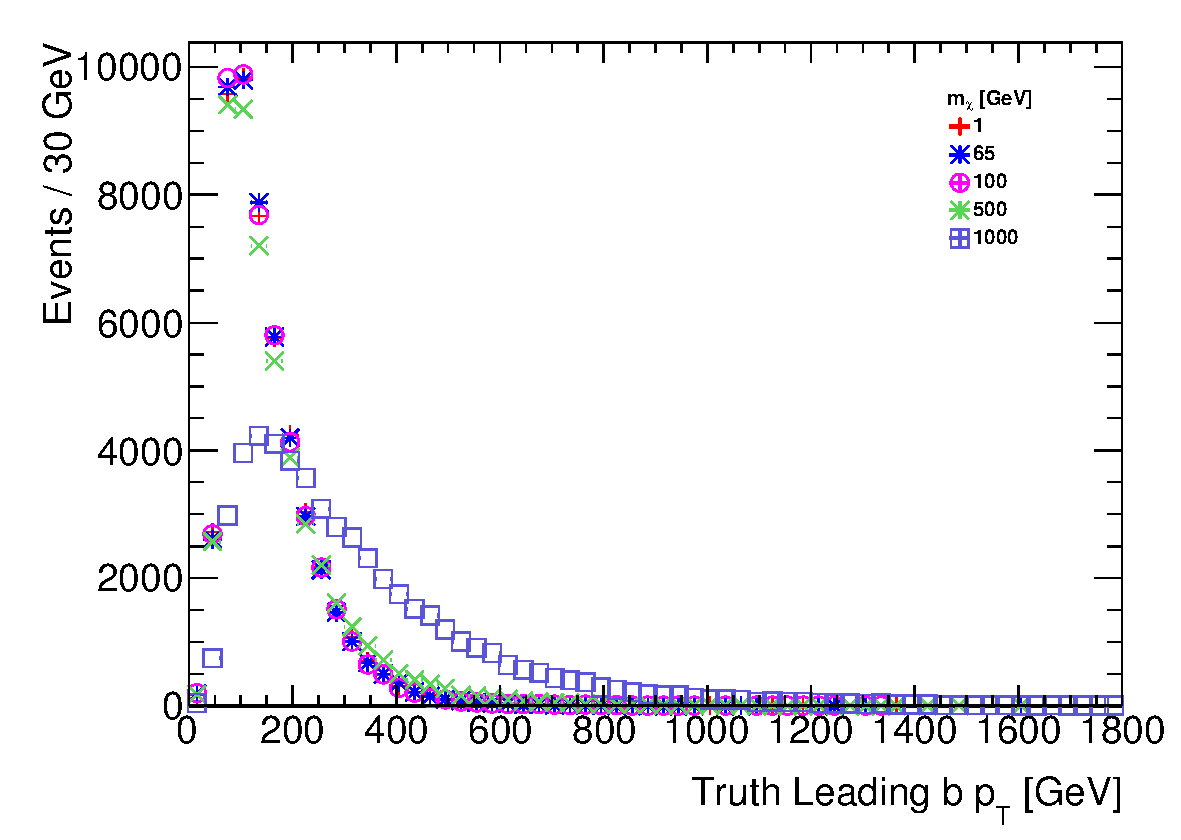
\includegraphics[width=0.75\linewidth]{figures/EW/monoH/zpzp1000/truth_leading_b_pt} %\label{fig:met_cmp_high}
	}\hfill
	\subfloat[Leading $b-$jet pseudorapidity]{
		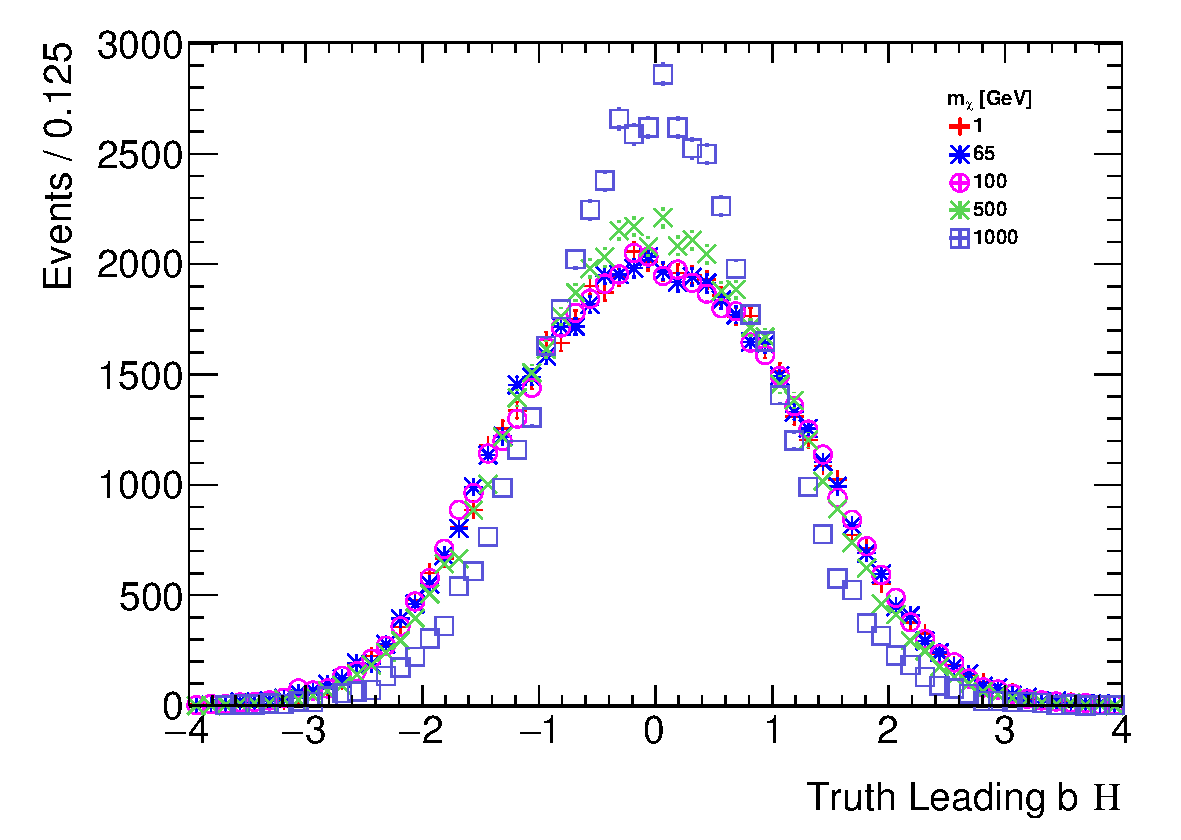
\includegraphics[width=0.75\linewidth]{figures/EW/monoH/zpzp1000/truth_leading_b_eta} %\label{fig:met_cmp_low}
	}\hfill
%	\hfill
%	\subfloat[Leading $b-$jet transverse momentum]{
%		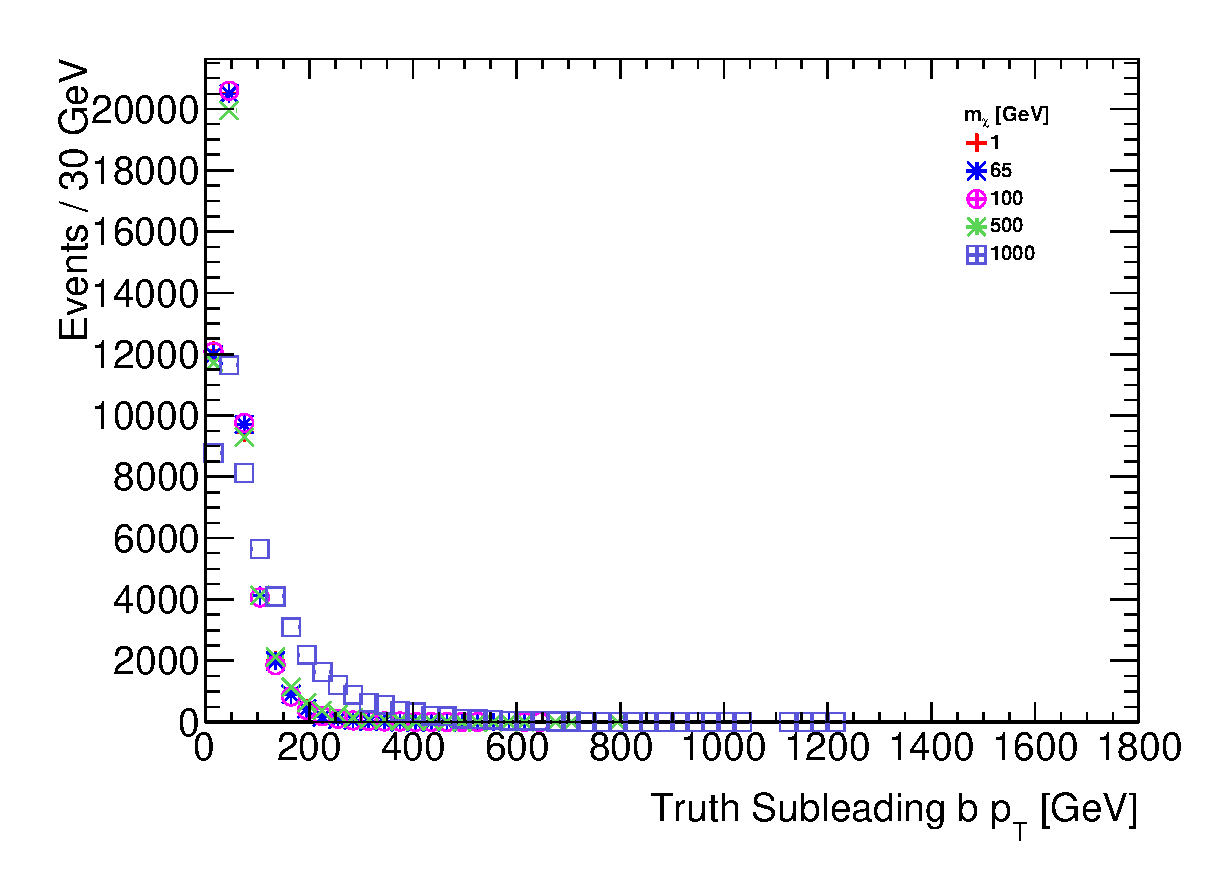
\includegraphics[width=0.95\linewidth]{figures/EW/monoH/zpzp1000/truth_subleading_b_pt} %\label{fig:met_cmp_high}
%	}
%	\hfill
%	\subfloat[Leading $b-$jet pseudorapidity]{
%		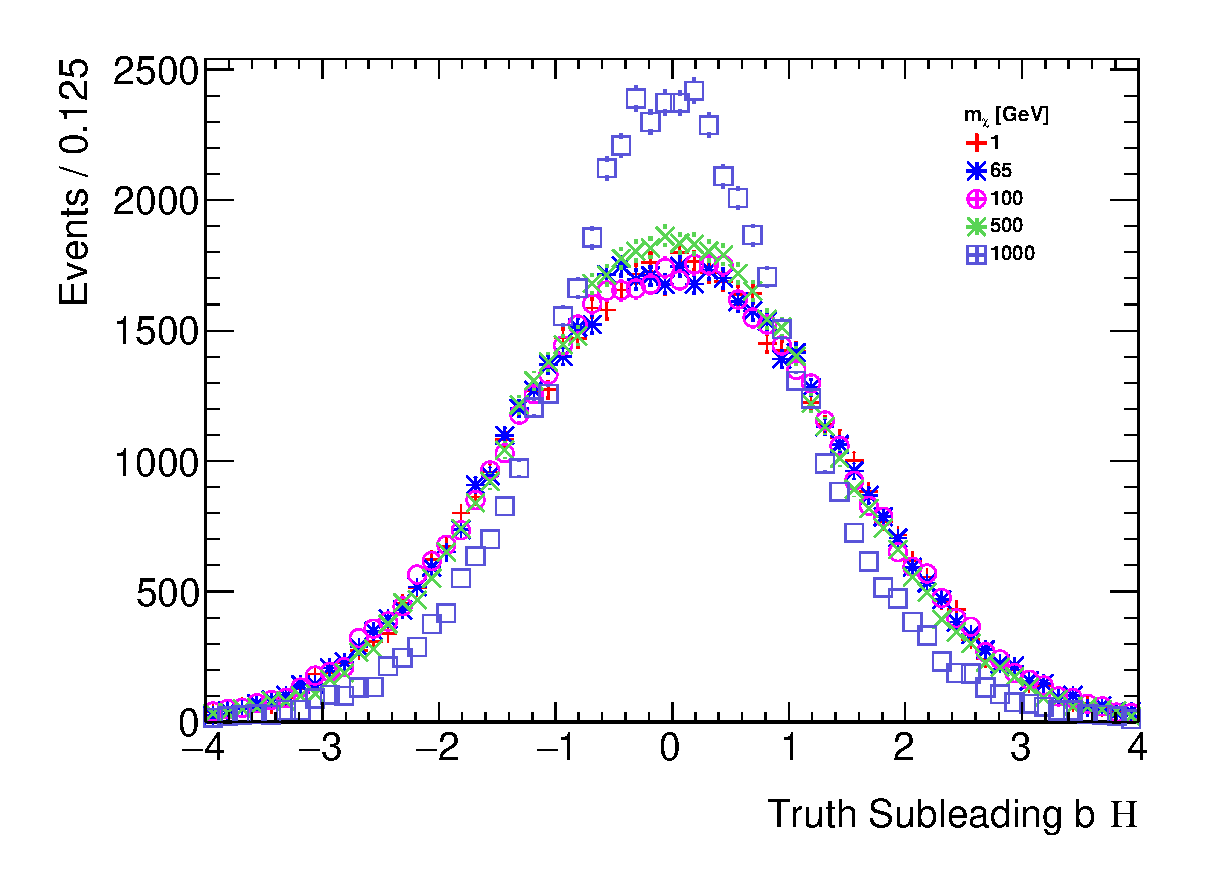
\includegraphics[width=0.95\linewidth]{figures/EW/monoH/zpzp1000/truth_subleading_b_eta} %\label{fig:met_cmp_low}
%	}
%	\hfill
	\subfloat[\text{Angular separation of the two leading $b$-jets}]{
		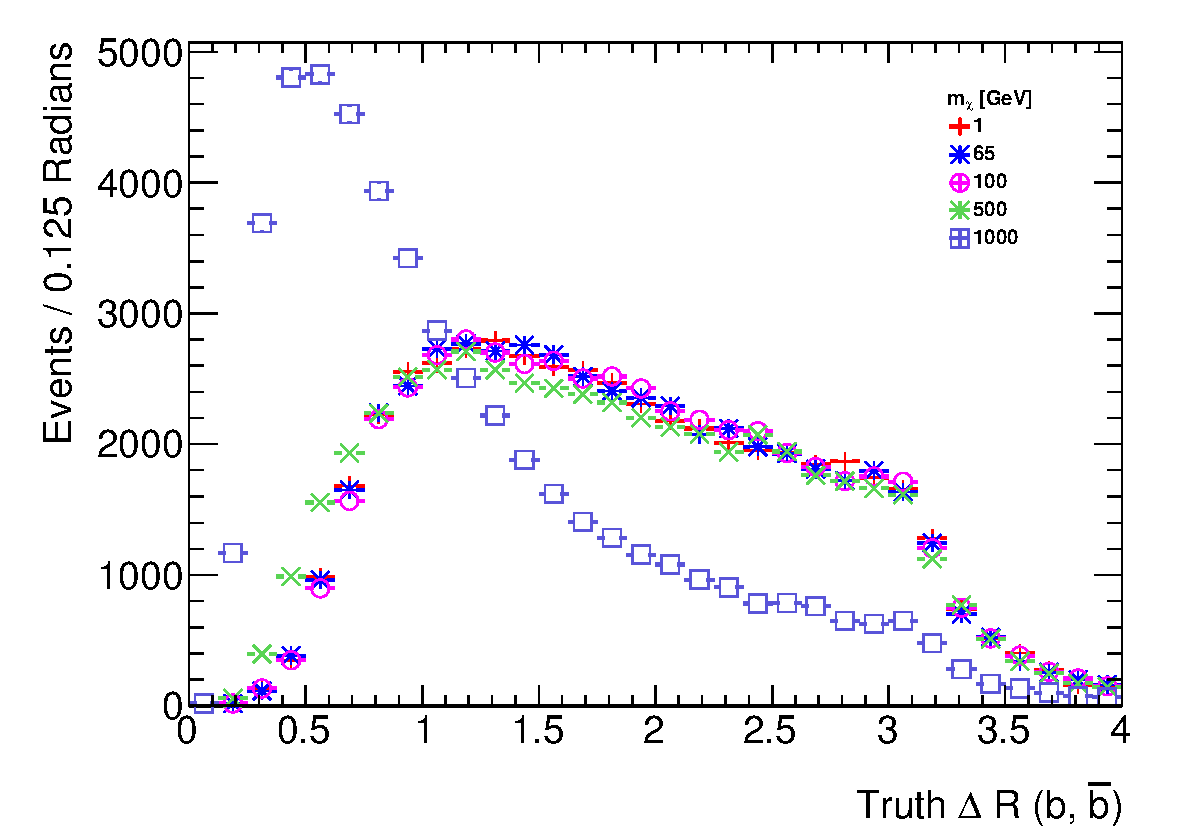
\includegraphics[width=0.75\linewidth]{figures/EW/monoH/zpzp1000/truth_bb_deltar} %\label{fig:met_cmp_low}
	}
	\caption{Comparison of the kinematic distributions for the two leading jets from the Higgs decay in the vector \Zprime simplified model, 
		when fixing the \Zprime mass to 1000~\gev and varying the DM mass. 
		\label{fig:VectorHbb_1000}}
\end{figure}



%%%%\clearpage

\subsection{\MET+Higgs from a scalar mediator}

A real scalar singlet $S$ coupling to DM can be introduced as a portal between SM and the dark sector 
through the Higgs field. The most general scalar potential is detailed in Ref.~\cite{O'Connell:2006wi}, 
including terms that break \Ztwo. 
The \Ztwo symmetry, which causes the new scalar to also be a DM candidate, is not covered in this report, but follows Ref.~\cite{Carpenter:2013xra}
introducing an additional coupling to DM that breaks \Ztwo and leads to a new invisible decay of $S$. 
For this reason, no symmetry is broken and no new interactions arise, so there is no dependence on the vacuum
expectation value of $S$: a shift in the field leads to a redefinition of the model couplings. 
The new scalar $S$ mixes with the SM Higgs boson, and couples to DM through a Yukawa term $y_\chiDM$. 
The relevant terms in the scalar potential are:

\begin{align}
&V \supset a |H|^2 S + b |H|^2 S^2 + \lambda_h |H|^4 \notag \\
& \;\;\longrightarrow \tfrac{1}{2} a (h +  v)^2 S + \tfrac{1}{2}b (h +  v)^2 S^2 + \frac{\lambda_h}{4} (h +  v)^4 ,
\label{singlethiggsmix}
\end{align}
where $a,b$ are new physics couplings and $\lambda_h$ is the Higgs quartic coupling.  

The additional Lagrangian terms for this model are: 

\be \label{LintScalar2}
\mathcal{L} \supset - y_\chiDM \bar\chiDM \chiDM (  \cos\theta\:S - \sin\theta\: h ) - \frac{m_q}{v} \bar q q (\cos\theta\: h + \sin\theta\: S )  \,
\ee
where $\theta$ is the mixing angle between the Higgs boson and the new scalar.

Mono-Higgs signals in this second model arise through processes shown in Fig.~\ref{fig:feyn_prod_monoH_S} (a,b), or through 
the radiation of a Higgs boson from the  $t$ quark in the production loop, in Fig.~\ref{fig:feyn_prod_monoH_S} (c). 
The first two processes depend on the $h^2 S$ and $h S^2$ cubic terms in Eq.~\eqref{singlethiggsmix}.  
At leading order in $\sin\theta$, these terms are:

\be
V_{\rm cubic} \approx \frac{\sin\theta}{v} ( 2 m_h^2 + m_S^2) h^2 S  + b \, v \, h \, S^2 + ...
\ee
with $a$ and $\lambda_h$ expressed in terms of $\sin\theta$ and $m_h^2$, respectively.  
At leading order of $\sin\theta$, the $h^2 S$ term is fixed once the mass eigenvalues $m_h, m_S$ 
and mixing angle are specified.  The $h\,S^2$ term is not fixed and remains a free parameter of the model, depending on 
the new physics coupling $b$. 

This model also has mono-X signatures through $h/S$ mixing. This model is related to the scalar model discussed in Sec.~\ref{sec:monojet_scalar}
in the case of $m_S \gg m_h$ or $m_h \gg m_S$ and  \mMed equal to the lighter of the two masses, albeit with different mono-Higgs signatures
due to the $h S^2$ vertex. 

\subsubsection{Parameter scan}

The model is described by five parameters: 

\begin{enumerate}
	\item the Yukawa coupling of heavy scalar to dark matter, \gDM (also referred to as $y_\chiDM$) 
	\item the mixing angle between heavy scalar and SM-like Higgs boson, $\sin\theta$;
	\item the new physics coupling, $b$;
	\item mass of heavy scalar, $m_{S}$, also termed \mmed;
	\item mass of dark matter. \mDM;
	%(also referred to as $m_{\.chiDM}$)
\end{enumerate}

The mixing angle is constrained from current Higgs data
to satisfy $\cos\theta = 1$ within 10\% and therefore $\sin\theta \lesssim 0.4$. This provides a starting point 
for the parameter scan in this model: we recommend to set $\sin\theta = 0.3$. 

\begin{figure}[hbpt!]
	\begin{center}
		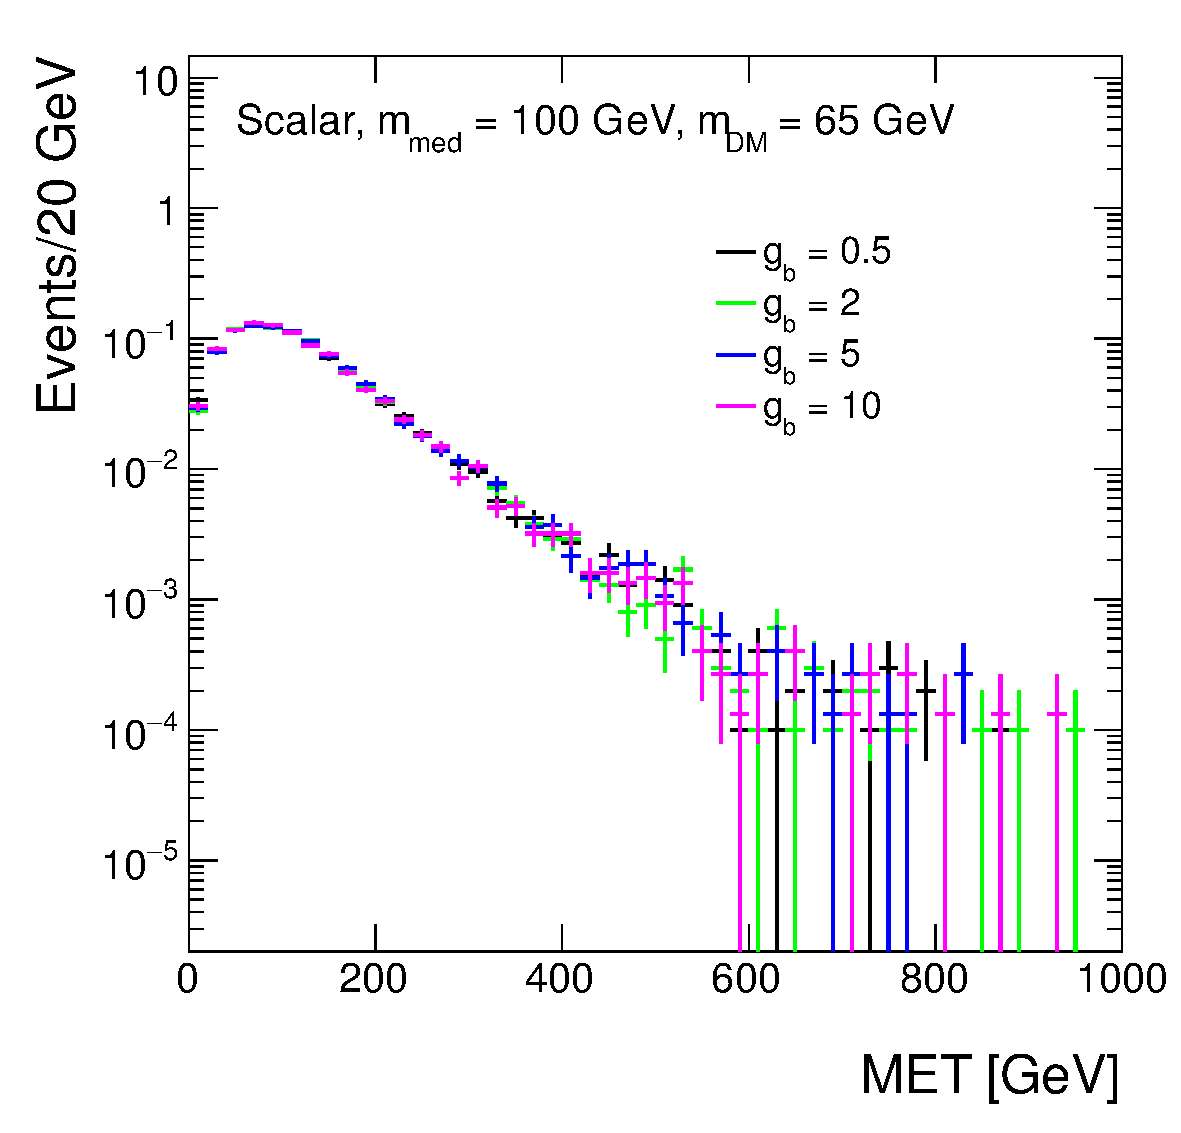
\includegraphics[width=0.75\linewidth]{figures/EW/monoH/s_gb_65_100_04_MET_et_Log}\\
		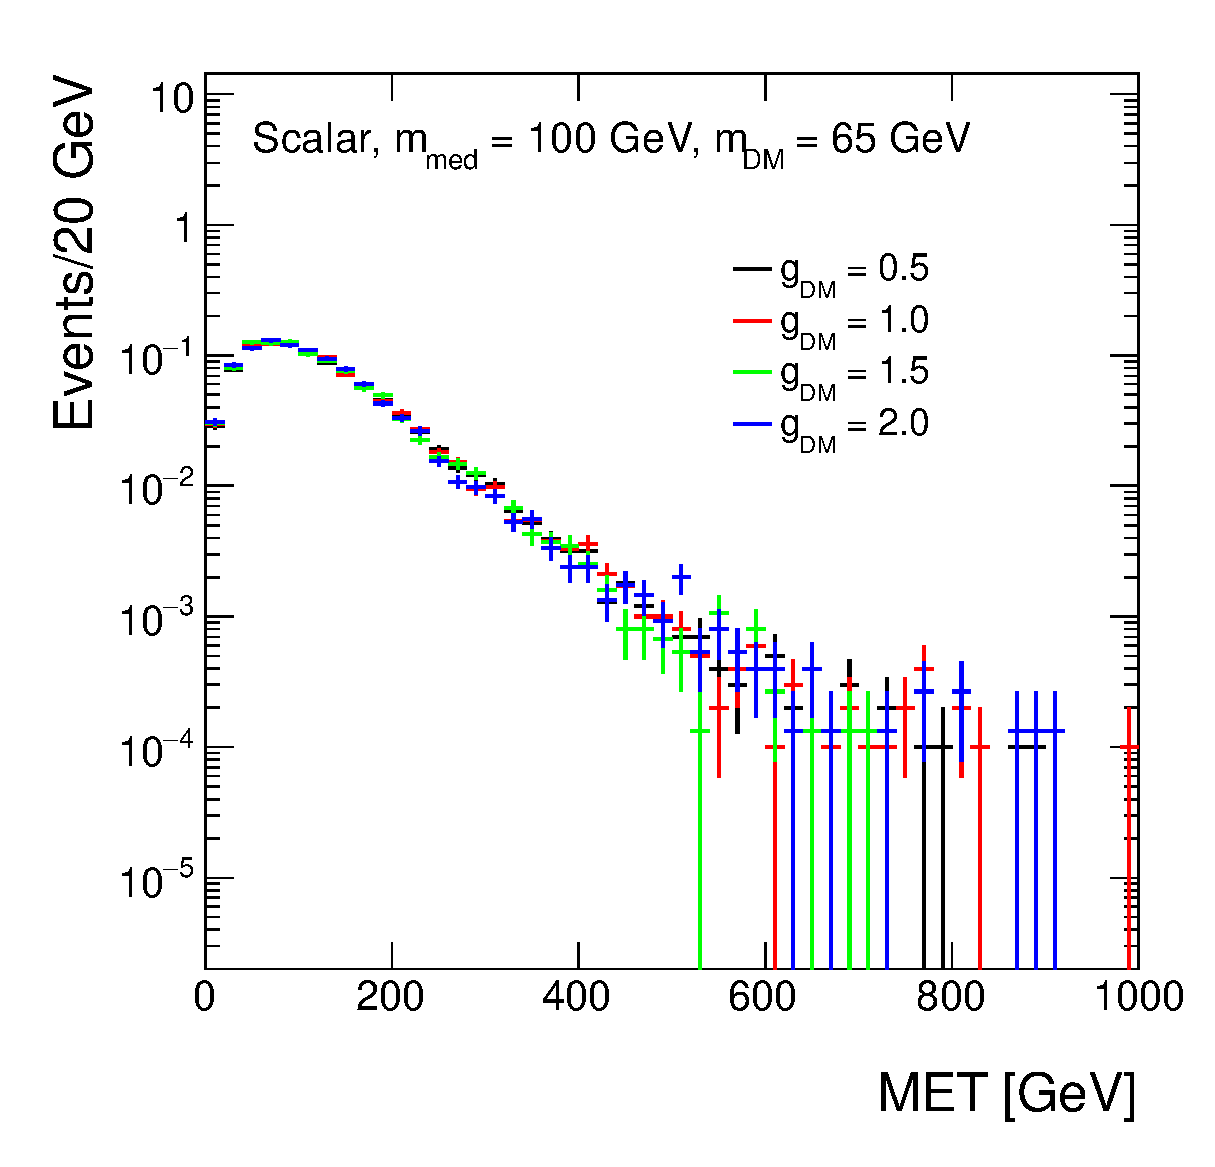
\includegraphics[width=0.75\linewidth]{figures/EW/monoH/s_gdm_MET_et_Log}
		\caption{Missing transverse momentum distributions at generator level in the scalar 
			mediator scenario, for different values of: the new physics coupling $g_b$ (left),
			and the mediator-dark matter coupling \gDM (right).
			\label{fig:metScalarCoupling}}
	\end{center}
\end{figure}

Figure~\ref{fig:metScalarCoupling2} shows that
there is no dependence of the kinematics from the value of this angle, and different values can be obtained via rescaling
the results for this mixing angle according to the relevant cross-section. It can also be observed from Figures~\ref{fig:metScalarMass} and~\ref{fig:metScalarCoupling} 
that the kinematics of this model follows that of the equivalent jet+\MET model: only small changes are observed
in the on-shell region, while the relevant distributions diverge when the mediator is off-shell. 
For this reason, the same grid in \mmed, \mdm as for the scalar mediator
of the jet+\MET search (Table~\ref{tab:mDMmMedScan_SP}) is chosen as a starting point. 
%\Todo{Estimate the sensitivity and possibly prune parameter scan.}
The Yukawa coupling to DM $y_{DM}$ is set to 1, the 
new physics coupling between scalar and SM Higgs $b$ = 3. Results for other values can be obtained via a 
rescaling of the results for these parameters. 
%More detailed studies are required to estimate the reach of the analysis with respect to all points in the grid
%and therefore decide on a smaller set of grid points to be generated; 
%those are left to the individual analyses. 



\begin{figure}[hbpt!]
	\begin{center}
		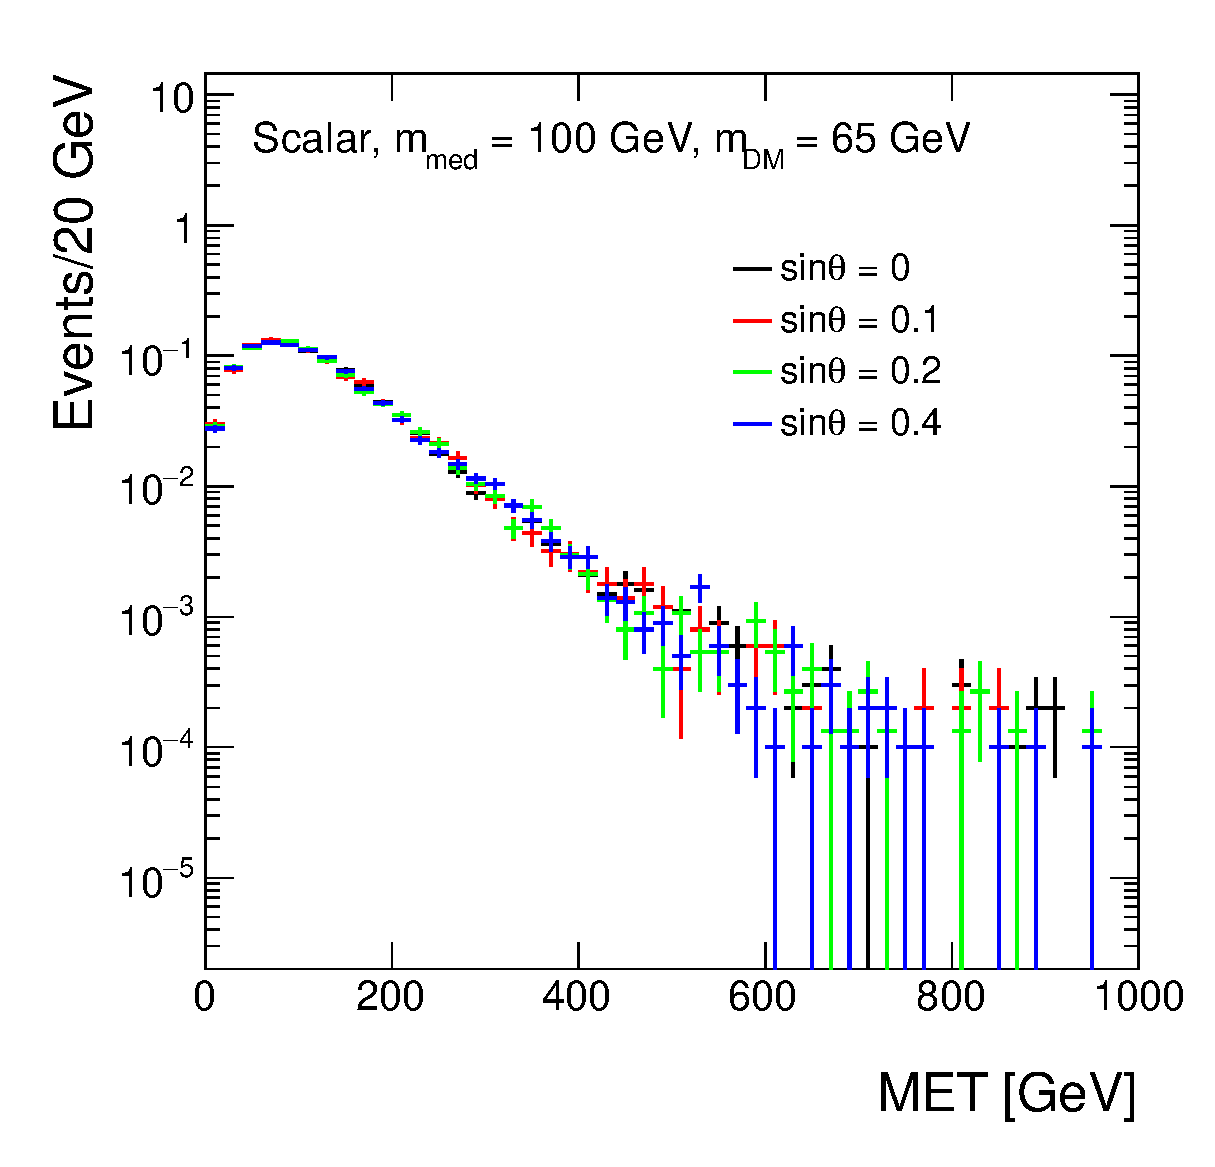
\includegraphics[width=0.75\linewidth]{figures/EW/monoH/s_theta_65_100_2_MET_et_Log}
		\caption{Missing transverse momentum distributions at generator level in the scalar 
			mediator scenario: for different values of the mixing angle $\sin\theta$.
			\label{fig:metScalarCoupling2} }
	\end{center}
\end{figure}

\begin{figure}[hbpt!]
	\begin{center}
		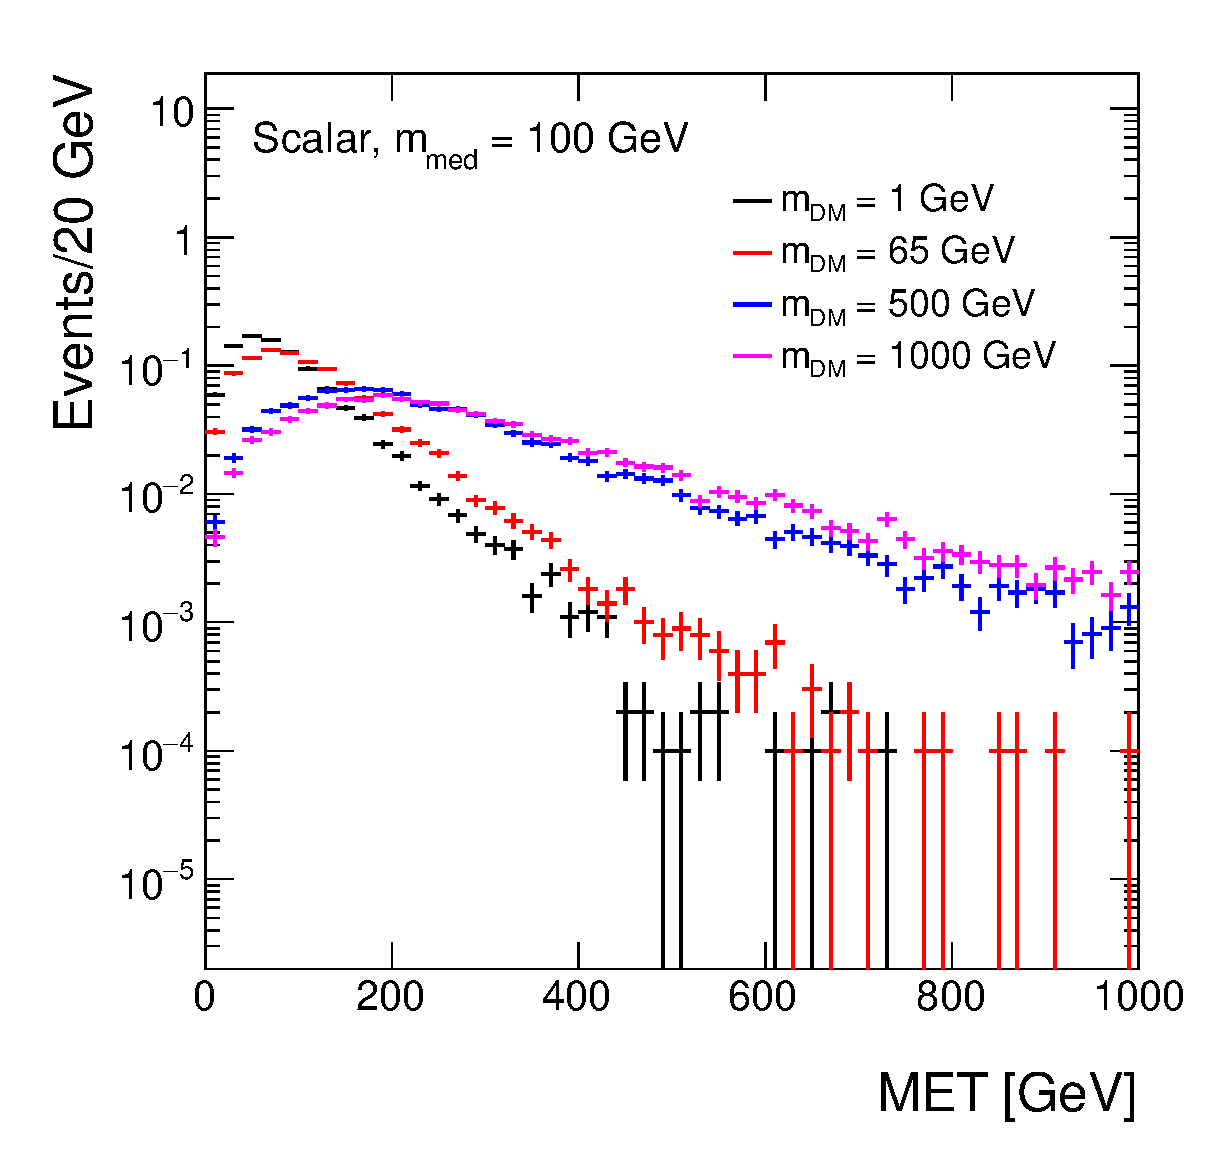
\includegraphics[width=0.75\linewidth]{figures/EW/monoH/scalar_100_MET_et_Log}\\
		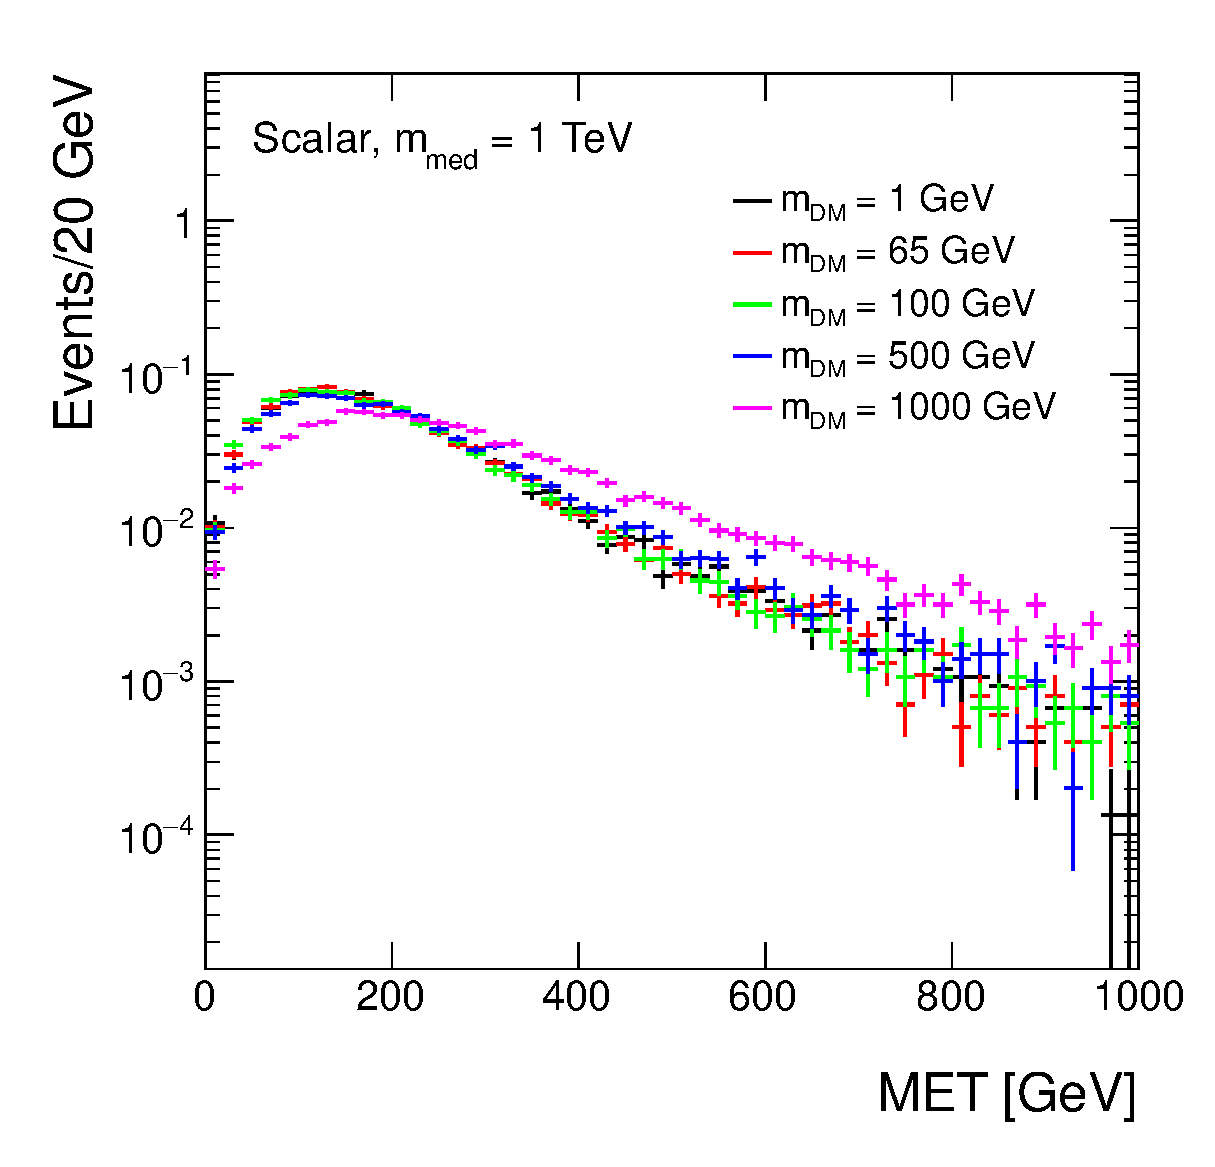
\includegraphics[width=0.75\linewidth]{figures/EW/monoH/scalar_1000_MET_et_Log}
		\caption{Missing transverse momentum distributions at generator level in the scalar 
			mediator scenario: for different values of the dark matter mass \mDM 
			and a mediator mass of $\mMed = 100~\gev$ (left) and $\mMed = 1~\tev$ (right).
			\label{fig:metScalarMass}}
	\end{center}
\end{figure}

Figs. ~\ref{fig:ScalarHbb_100} and ~\ref{fig:ScalarHbb_1000} show the kinematic distributions for the two leading jets
in the $H \to \bar b b$ decay channel, for two values of the mediator mass and varying the DM mass.  

\begin{figure}[hbpt!]
	\centering
	\subfloat[Leading $b-$jet transverse momentum]{
		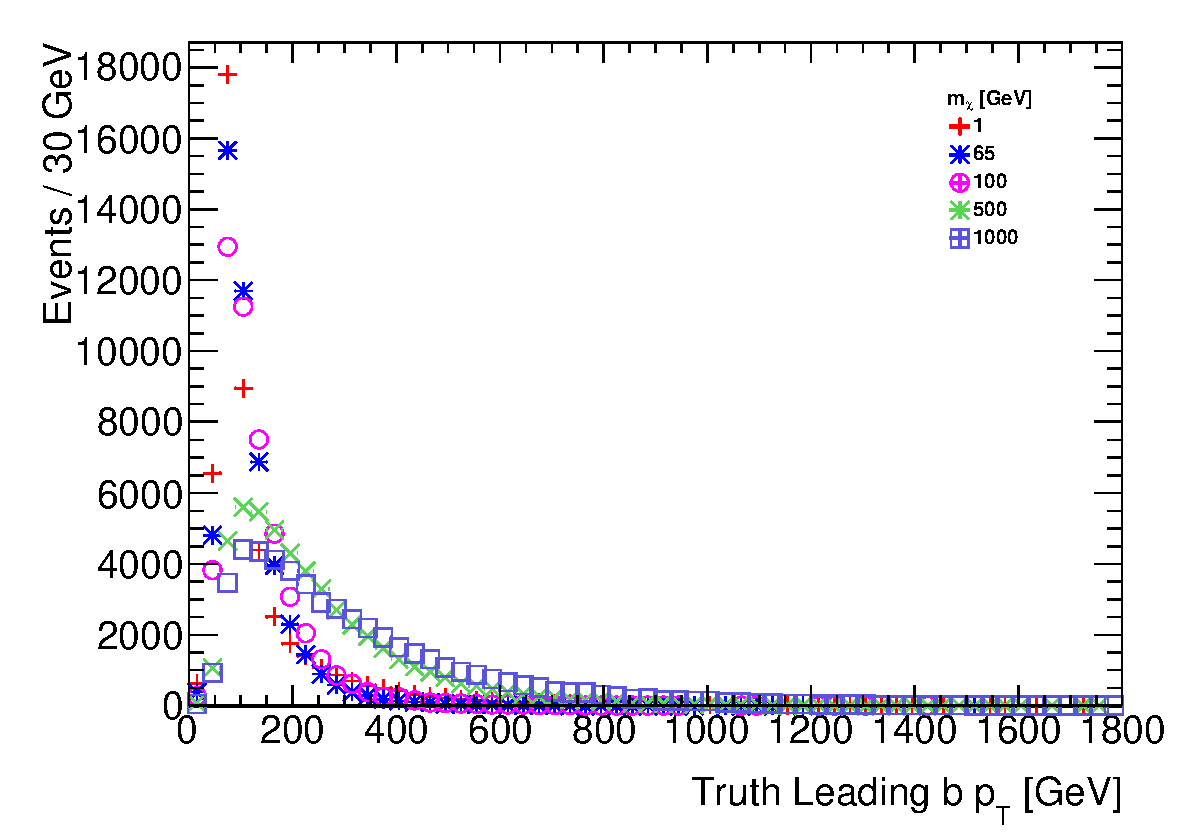
\includegraphics[width=0.75\linewidth]{figures/EW/monoH/scalar100/truth_leading_b_pt} %\label{fig:met_cmp_high}
	}
	\hfill
	\subfloat[Leading $b-$jet pseudorapidity]{
		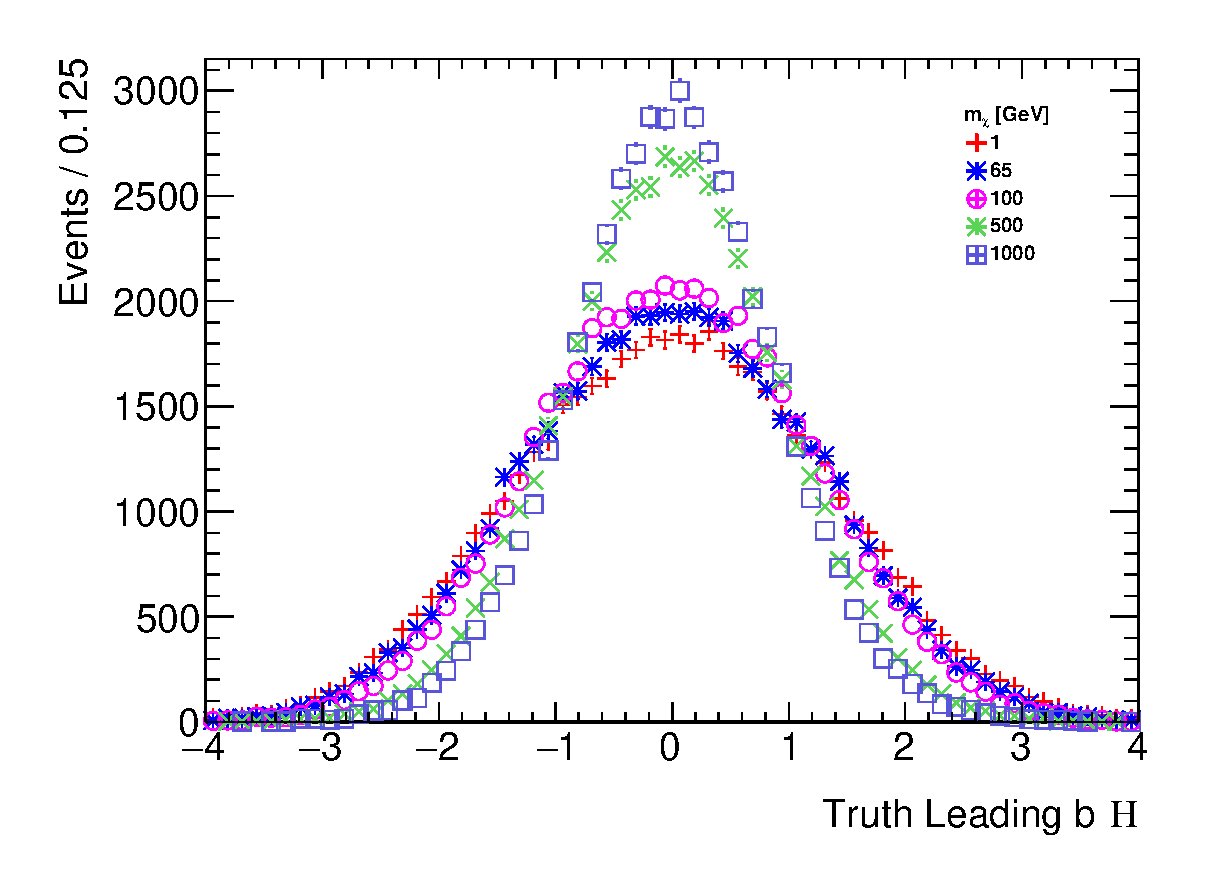
\includegraphics[width=0.75\linewidth]{figures/EW/monoH/scalar100/truth_leading_b_eta} %\label{fig:met_cmp_low}
	}\hfill
%	\hfill
%	\subfloat[Leading $b-$jet transverse momentum]{
%		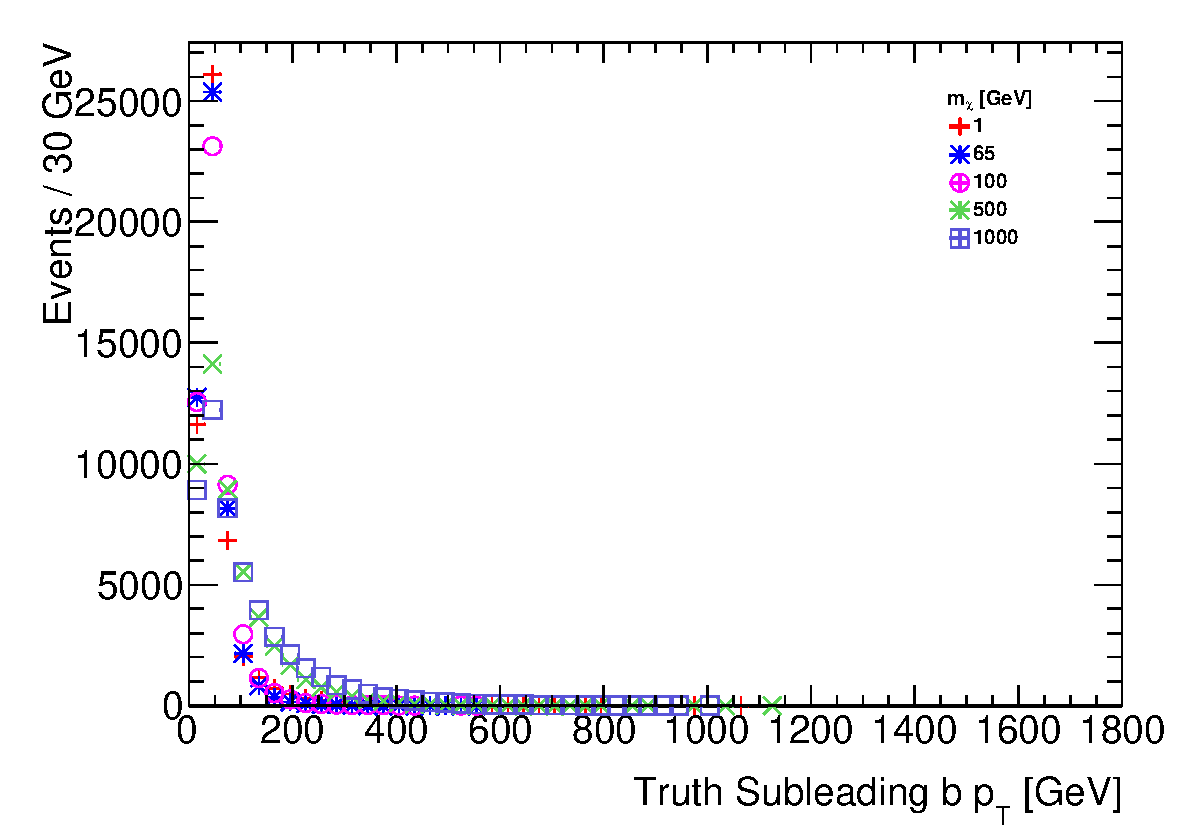
\includegraphics[width=0.95\linewidth]{figures/EW/monoH/scalar100/truth_subleading_b_pt} %\label{fig:met_cmp_high}
%	}
%	\hfill
%	\subfloat[Leading $b-$jet pseudorapidity]{
%		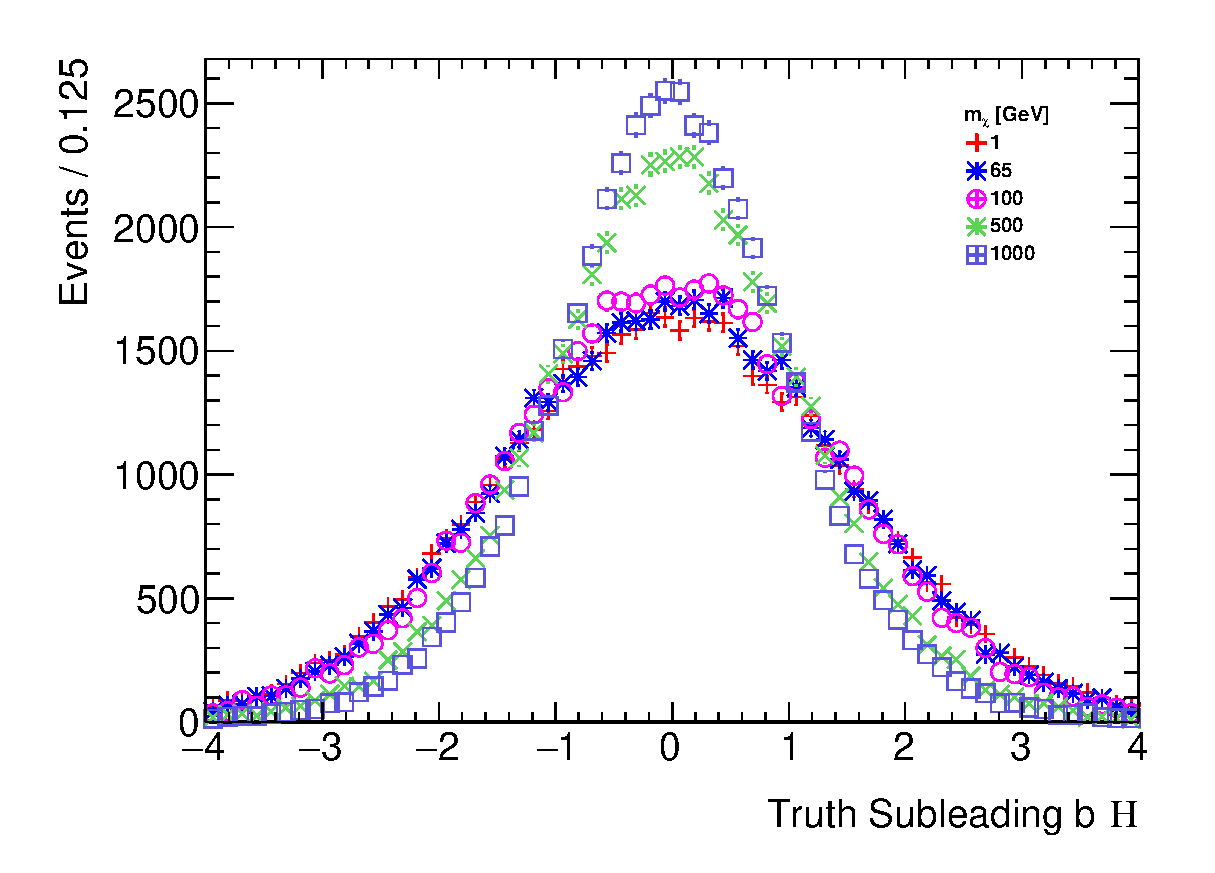
\includegraphics[width=0.95\linewidth]{figures/EW/monoH/scalar100/truth_subleading_b_eta} %\label{fig:met_cmp_low}
%	}
	\subfloat[Angular distance between the two leading $b-$jets]{
		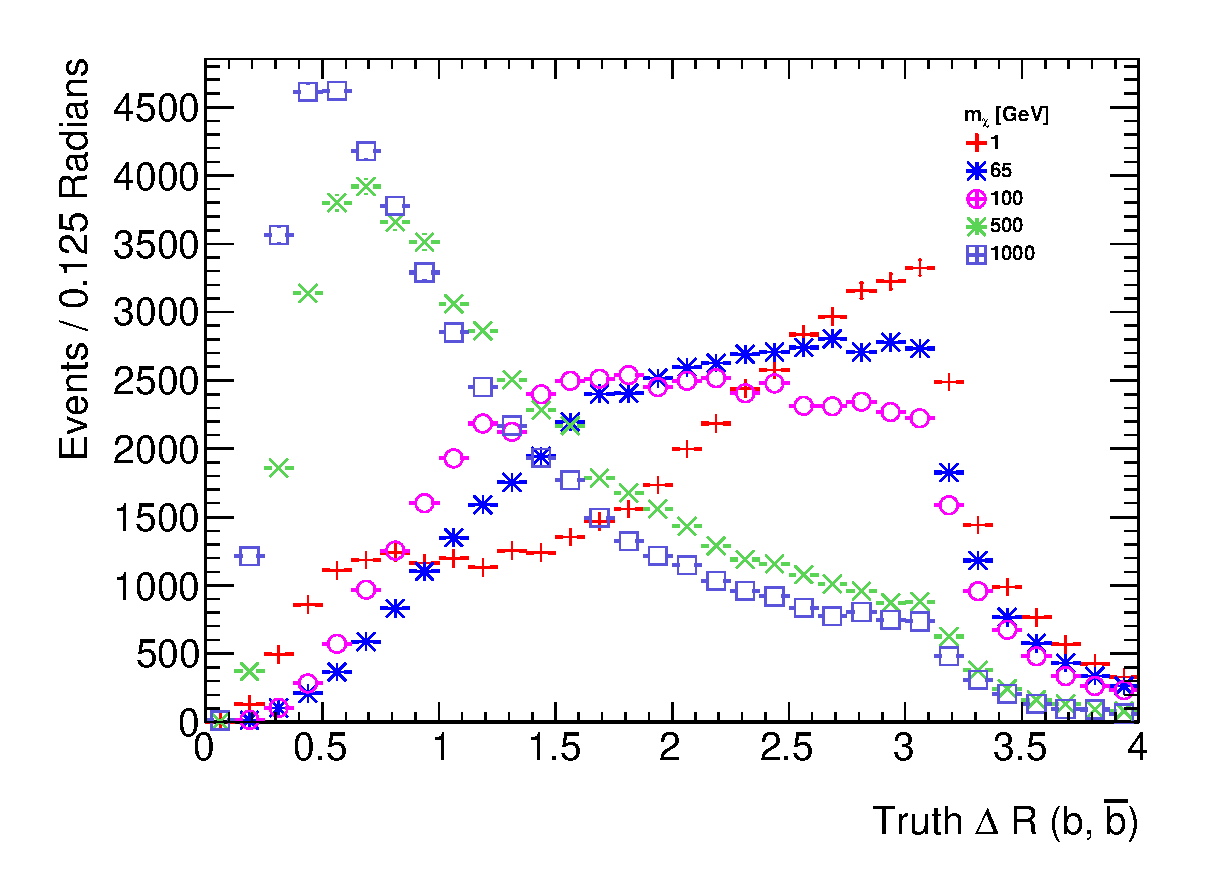
\includegraphics[width=0.75\linewidth]{figures/EW/monoH/scalar100/truth_bb_deltar} %\label{fig:met_cmp_low}
	}

	\caption{Comparison of the kinematic distributions for the two leading jets from the Higgs decay in the scalar simplified model, 
		when fixing the new scalar mass to 100~\gev and varying the DM mass. 
		\label{fig:ScalarHbb_100}}
\end{figure}

\begin{figure}[hbpt!]
	\centering
	\subfloat[Leading $b-$jet transverse momentum]{
		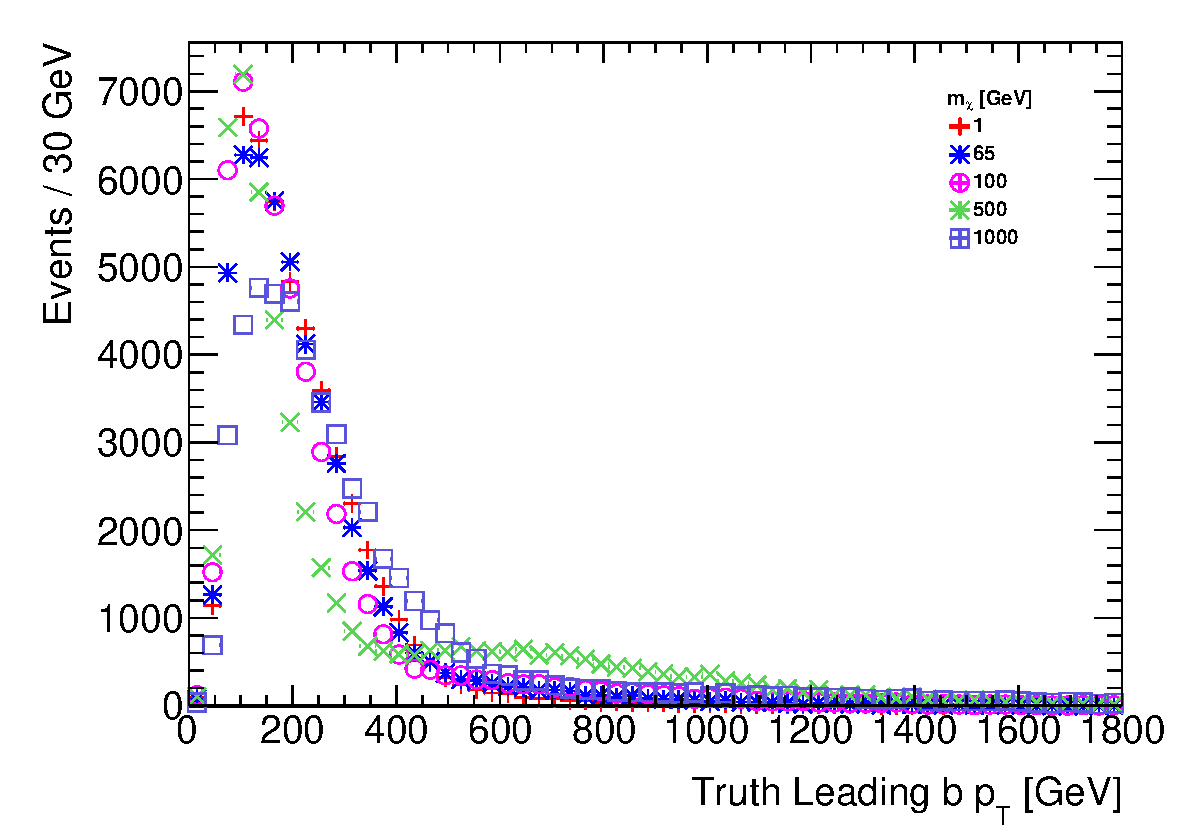
\includegraphics[width=0.75\linewidth]{figures/EW/monoH/scalar1000/truth_leading_b_pt} %\label{fig:met_cmp_high}
	}
	\hfill
	\subfloat[Leading $b-$jet pseudorapidity]{
		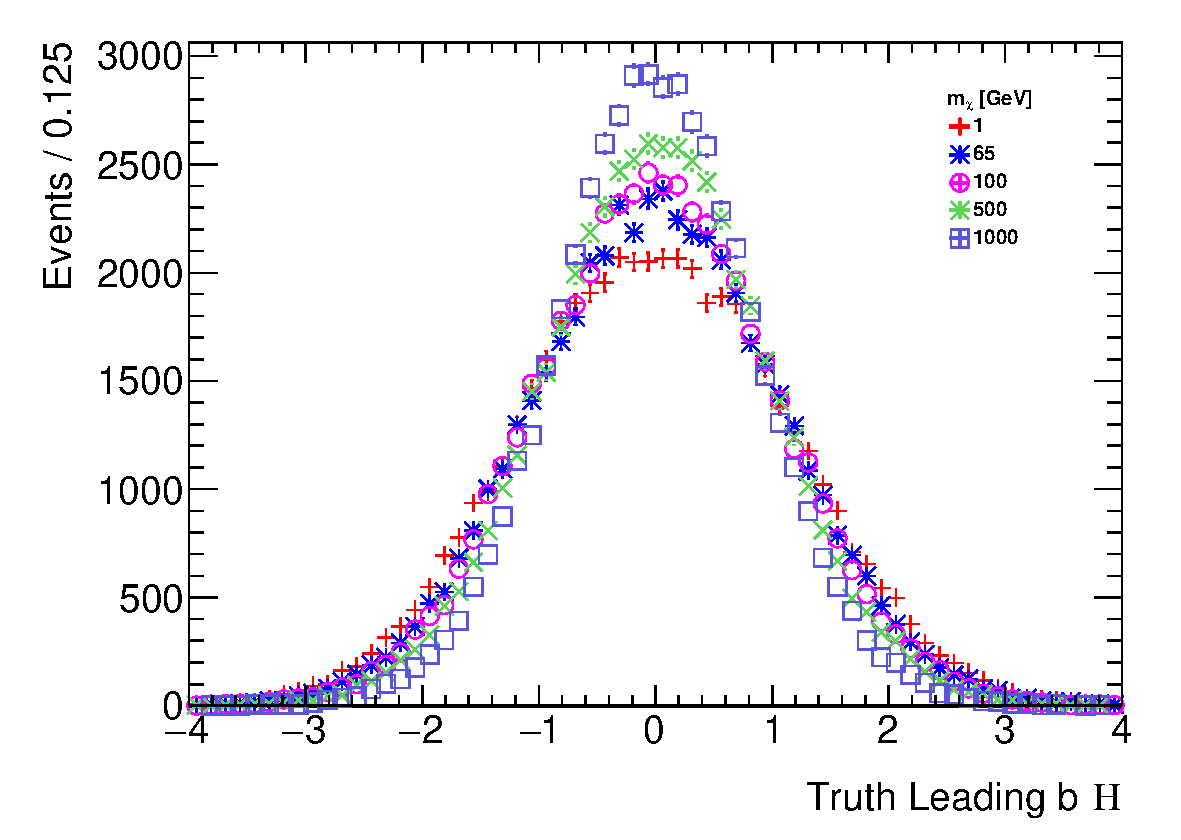
\includegraphics[width=0.75\linewidth]{figures/EW/monoH/scalar1000/truth_leading_b_eta} %\label{fig:met_cmp_low}
	}
%	\hfill
%	\subfloat[Leading $b-$jet transverse momentum]{
%		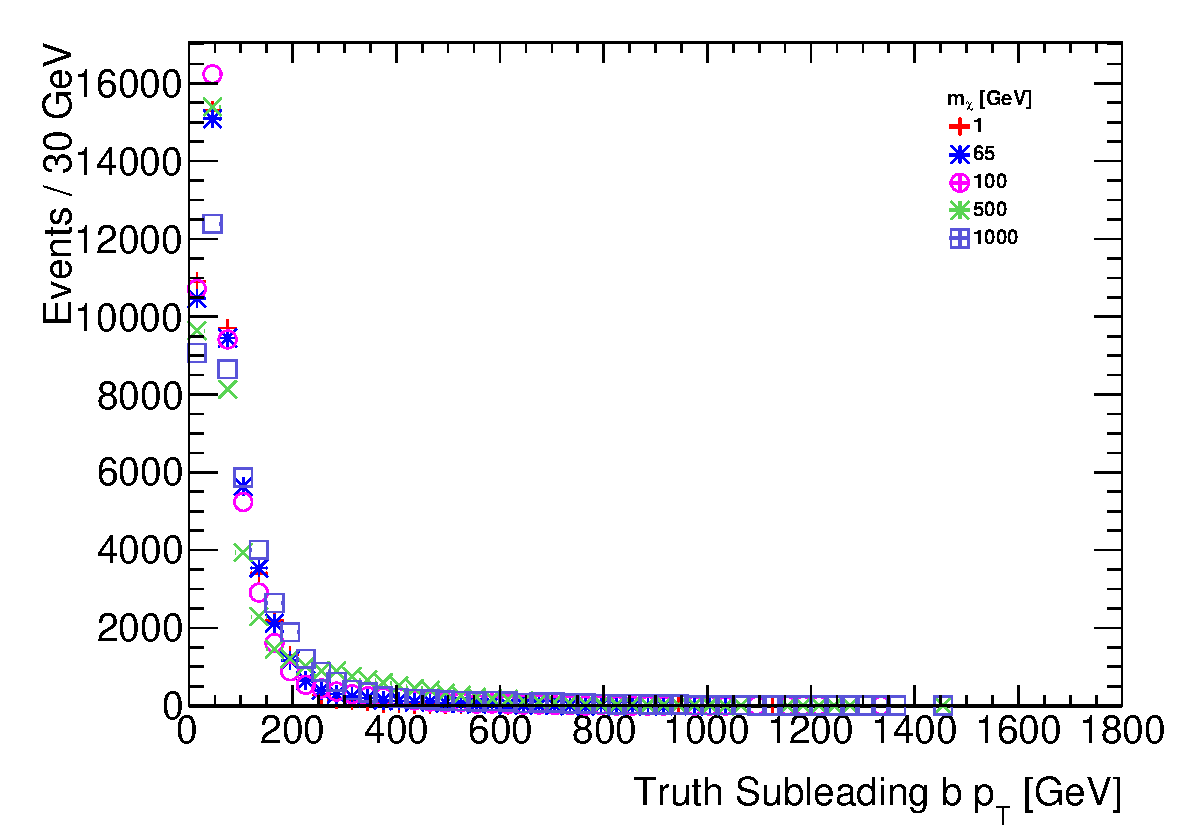
\includegraphics[width=0.95\linewidth]{figures/EW/monoH/scalar1000/truth_subleading_b_pt} %\label{fig:met_cmp_high}
%	}
%	\hfill
%	\subfloat[Leading $b-$jet pseudorapidity]{
%		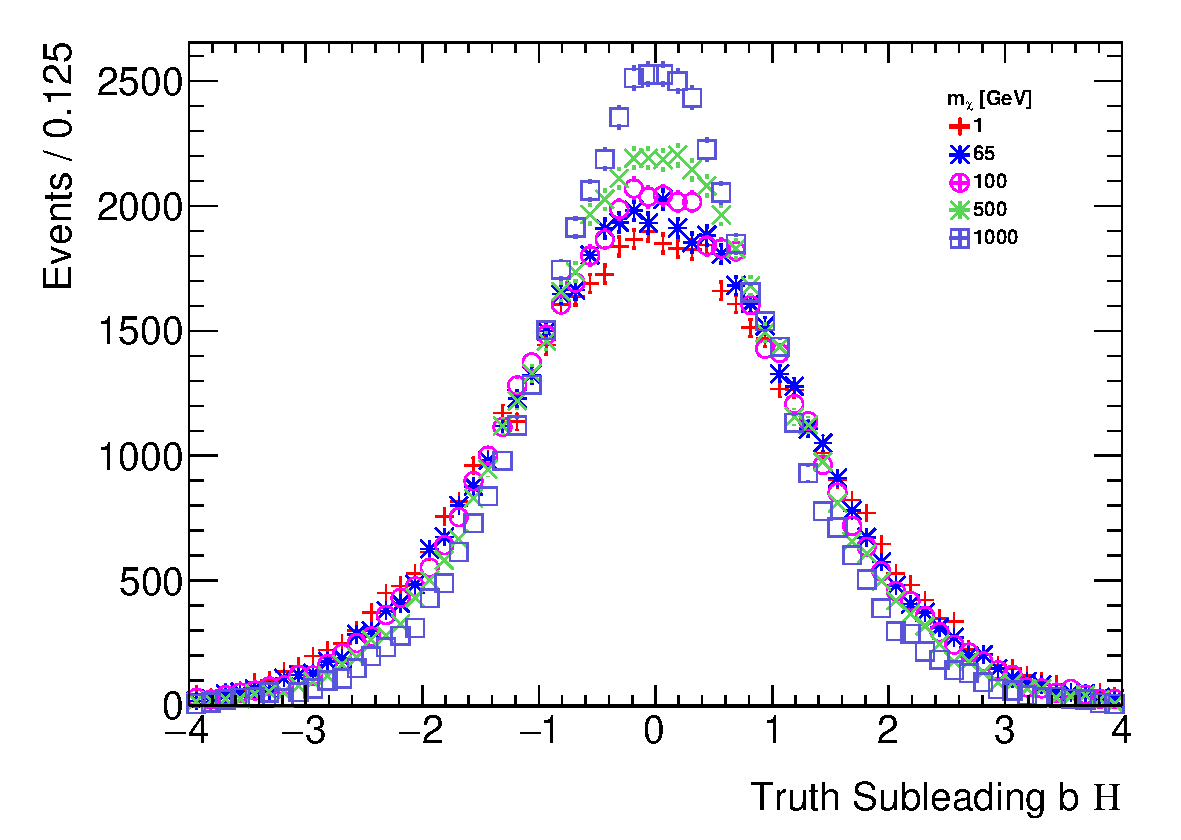
\includegraphics[width=0.95\linewidth]{figures/EW/monoH/scalar1000/truth_subleading_b_eta} %\label{fig:met_cmp_low}
%	}
	\hfill
	\subfloat[Angular distance between the two leading $b-$jets]{
		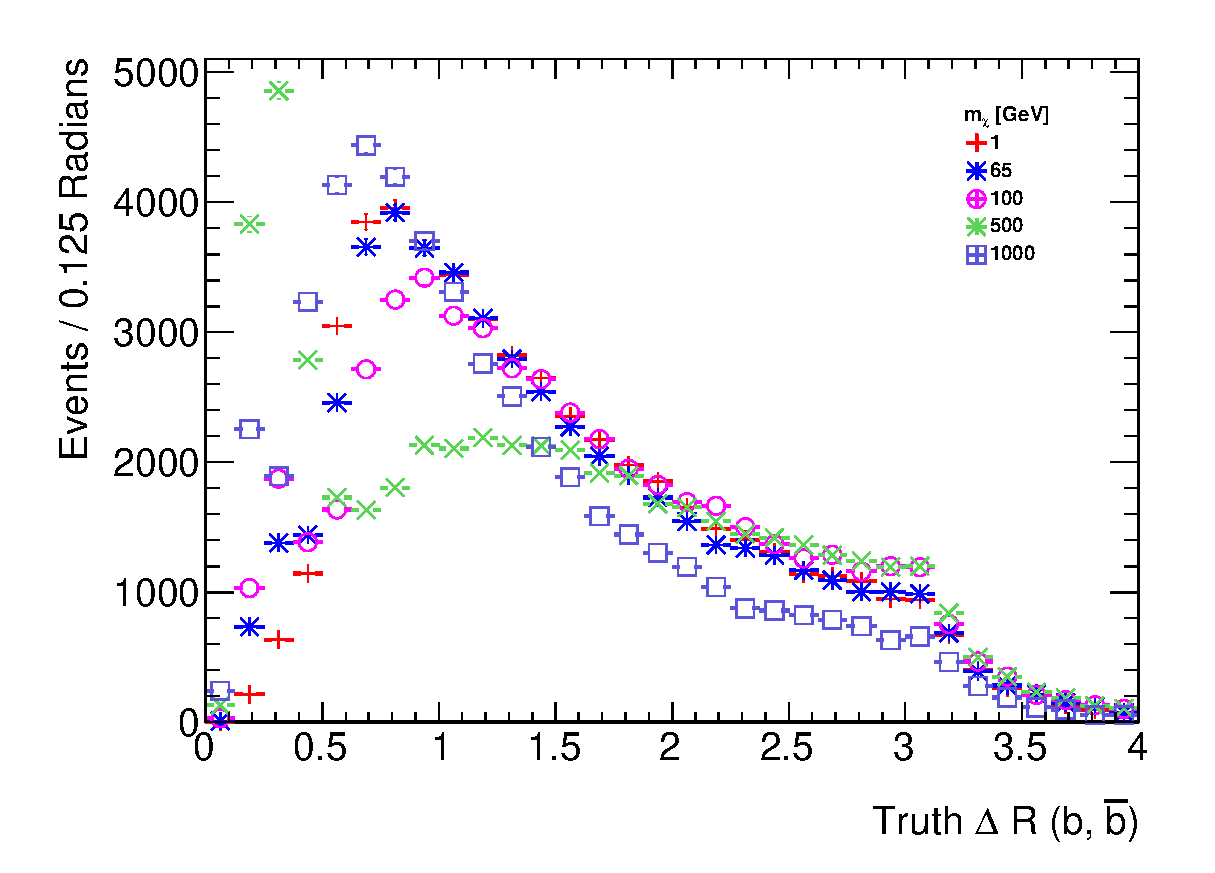
\includegraphics[width=0.75\linewidth]{figures/EW/monoH/scalar1000/truth_bb_deltar} %\label{fig:met_cmp_low}
	}
	\caption{Comparison of the kinematic distributions for the two leading jets from the Higgs decay in the scalar simplified model, 
		when fixing the new scalar mass to 1000~\gev and varying the DM mass. 
		\label{fig:ScalarHbb_1000}}
\end{figure}


%%%
\subsection{Higgs+\MET signal from 2HDM model with a \Zprime and a new pseudoscalar}

In this simplified model~\cite{Berlin:2014cfa}, a new \Zprime resonance decays to a Higgs boson $h$ 
plus a heavy pseudoscalar state 
$A^0$ in the 2HDM framework, which in turn decays to a DM pair. This model is 
represented in the diagram in Fig. \ref{fig:feyn_prod_monoH} (b).


The motivation for coupling the dark matter to the pseudoscalar is that dark matter coupling to a Higgs or \Zprime boson is generically 
constrained by other signal channels and direct detection.
A reason to consider this model
is that it has different kinematics  due to the on-shell \Zprime production, 
where for heavy \Zprime masses the \MET and $p_T$ spectra are much harder.
This model can satisfy electroweak precision tests and constraints from dijet resonance searches, 
and still give a potentially observable Higgs+\MET signal.
 
 This model comprises two doublets, where $\Phi_u$ couples to up-type quarks and $\Phi_d$ couples to down-type
 quarks and leptons:

 \begin{equation}
 -{\mathcal{L}} \supset  y_u Q \tilde \Phi_u \bar u + y_d Q \Phi_d \bar d + y_e L \Phi_d \bar e  + {\rm h.c.}
 \end{equation}
 
 After electroweak symmetry breaking, the Higgs doublets attain vacuum expectation values $v_u$ and $v_d$, and in unitary gauge the doublets are parametrized as

 \begin{align}
 \Phi_d &= \frac{1}{\sqrt{2}}
 \begin{pmatrix}
 -\sin{\beta} \ H^+ \\ v_d - \sin{\alpha} \ h + \cos{\alpha} \ H - i \sin{\beta} \ A^0
 \end{pmatrix} 
 \quad , \nonumber \\
 \Phi_u &= \frac{1}{\sqrt{2}}
 \begin{pmatrix}
 \cos{\beta} \ H^+ \\ v_u + \cos{\alpha} \ h + \sin{\alpha} \ H + i \cos{\beta} \ A^0
 \end{pmatrix}
 \end{align}
 where $h,H$ are neutral CP-even scalars,
 $H^\pm$ is a charged scalar, and $A^0$ is a neutral CP-odd scalar. 
 In this framework, $\tan{\beta} \equiv v_u/v_d$, and $\alpha$ is the mixing angle that diagonalizes 
 the $h - H$ mass squared matrix. This model also contains an additional scalar singlet $\phi$
 that leads to spontaneous symmetry breaking. 
 %FIXME: this is an external constrain that may or may not be included 
%The masses of the remaining scalars $H, A^0, H^\pm$ are assumed to be 
%around or above $300$~\gev, respecting $b \to s \gamma$ constraints \cite{Branco:2011iw}.
We take $\alpha = \beta - \pi/2$, in the 
%alignment 
limit where $h$ has SM-like couplings to fermions and 
gauge bosons as per Ref.~\cite{Craig:2013hca}, and $\tan{\beta} \ge 0.3$ 
as implied from the perturbativity of the top Yukawa coupling. 
  %For the $ b \bar{b}$ decay channel, the signature of the signal we are searching for is a pair of boosted WIMPs recoiling against two $b$ jets. 
The Higgs vacuum expectation values lead to $Z-\Zprime$ mass mixing, with a small mixing parameter given by 
 \begin{align}
 \epsilon & \equiv \frac{1}{M_{\Zprime}^2 - M_Z^2} \frac{g g_z}{2 \cos{\theta_w}} ( z_d v_d^2 + z_u v_u^2) \nonumber \\
 & =  \frac{(M_Z^0)^2}{M_{\Zprime}^2 - M_Z^2} \frac{2 g_z \cos \theta_w}{g}  z_u \sin^2 \beta, 
 \label{eq:epsilon}
 \quad
 \end{align}
 where $z_i$ are the $\Zprime$ charges of the two Higgs doublets, and  $g$ and $g_z$ related to the mass-squared
 values in absence of mixing  $(M_Z^0)^2 = g^2(v_d^2+ v_u^2)/(4\cos^2{\theta_w}) $ and
 $(M_{Z'}^0)^2 = g_z^2 ( z_d^2 v_d^2 + z_u^2 v_u^2 + z_\Phi^2
 v_\Phi^2)$. %In the limit where $\alpha = \beta - \pi/2$,
    
The production cross section for this model scales as $(g_z)^2$, as the decay width for this process
to leading order in $\epsilon$ (Eq.~\ref{eq:epsilon}) is
\begin{equation}
%\Gamma_{\Zprime \to h A^0} =  (g_z \cos \alpha \cos \beta)^2 \frac{|p|}{24 \pi} \frac{|p|^2}{M_{\Zprime}^2}.
\Gamma_{\Zprime \to h A^0} =  (g_z \sin \beta \cos \beta)^2 \frac{|p|}{24 \pi} \frac{|p|^2}{M_{\Zprime}^2}.
\end{equation}
where the center of mass momentum for the decay products
$\displaystyle |p| = \frac{1}{2 M_{\Zprime}} \sqrt{ (M_{\Zprime}^2 - (m_h + m_{A^0})^2)
(M_{\Zprime}^2 - (m_h - m_{A^0})^2)}$.
The $\Zprime$ can also decay to $Zh$, leading to the same signature if the $Z$ decays invisibly. The partial width for this decay is:
\begin{equation}
%\Gamma_{Z' \to hZ}  = (g_z \cos \alpha \sin \beta)^2 \frac{|p|}{24 \pi} \left( \frac{ |p|^2 }{M_{Z'}^2} + 3 \frac{M_Z^2}{M_{Z'}^2} \right),
\Gamma_{Z' \to hZ}  = (g_z \sin \beta^2)^2 \frac{|p|}{24 \pi} \left( \frac{ |p|^2 }{M_{Z'}^2} + 3 \frac{M_Z^2}{M_{Z'}^2} \right),
\end{equation}. We recommend to generate these two decays separately and combine them at a later stage. 

%\frac{1}{2 M_{\Zprime}} \lambda^{1/2}(M_{\Zprime}^2,m_h^2, m_{A^0}^2)$, and
%$\lambda$ is the K\"{a}llen triangle function\sidenote{\vskip -2.5\baselineskip%\begin{align*}\lambda(c_1,c_2,c_3) \equiv&\;c_1^2 + c_2^2 + c_3^2\\ 
%						&- 2(c_1 c_2 + c_2 c_3 + c_3 c_1)\end{align*}}.
   
%  Diagonalizing the gauge
% boson mass matrix, the tree-level masses of the $Z$ and \Zprime bosons are given by
% \begin{align}
% M_Z^2 &\approx ( M_{Z}^0)^2  - \epsilon^2 \left[( M_{\Zprime}^0)^2 - ( M_{Z}^0)^2 \right] \nonumber \\
% M_{\Zprime}^2 &\approx ( M_{\Zprime}^0)^2 + \epsilon^2 \left[( M_{\Zprime}^0)^2 - ( M_{Z}^0)^2 \right]
% \quad ,
% \label{eq:Zpmasses}
% \end{align}
% where $(M_Z^0)^2 = g^2(v_d^2+ v_u^2)/(4\cos^2{\theta_w}) $ and
% $(M_{\Zprime}^0)^2 = g_z^2 ( z_d^2 v_d^2 + z_u^2 v_u^2 + z_\phi^2
% v_\phi^2)$ are the mass-squared values in the absence of mixing. The
% result above is accurate to order $\epsilon^2$, where $\epsilon$ is
% a small mixing parameter given by
% \begin{align}
% \epsilon & \equiv \frac{1}{M_{\Zprime}^2 - M_Z^2} \frac{g g_z}{2 \cos{\theta_w}} ( z_d v_d^2 + z_u v_u^2) \nonumber \\
% & =  \frac{(M_Z^0)^2}{M_{\Zprime}^2 - M_Z^2} \frac{2 g_z \cos \theta_w}{g}  z_u \sin^2 \beta.
% \label{eq:epsilon}
% \quad
% \end{align}
 
\subsubsection{Parameter scan}
 
 The model is described by five parameters:
 \begin{itemize}
 	\item the pseudoscalar mass $M_{A^0}$,
 	\item the DM mass \mDM,
 	\item the \Zprime mass, $M_{\Zprime}$,
        \item $\tan{\beta} (\equiv v_u/v_d)$,
 	\item the \Zprime coupling strength $g_z$. 
 \end{itemize}
% \Todo{What about Z' coupling to q and DM? CD: isn't this the DMV model?}
 
 To study the signal production and kinematic dependencies on these parameters, 
 we produced signal samples varying each of the five parameters through 
 \madgraph for the matrix element, \pythiaEight for the parton shower, and DELPHES\cite{deFavereau:2013fsa}  for a parameterized detector-level simulation.
 
 As seen in Fig.~\ref{fig:DMH_tanbeta}, variations of $\tan{\beta}$ does not lead to any kinematic 
 difference and the production cross section simply scales as a function of $\tan{\beta}$. Hence 
we recommend to fix $\tan{\beta}$ to unity in the signal generation. 


\begin{figure}[htpb!]
\centering
\subfloat[\MET distribution]{
	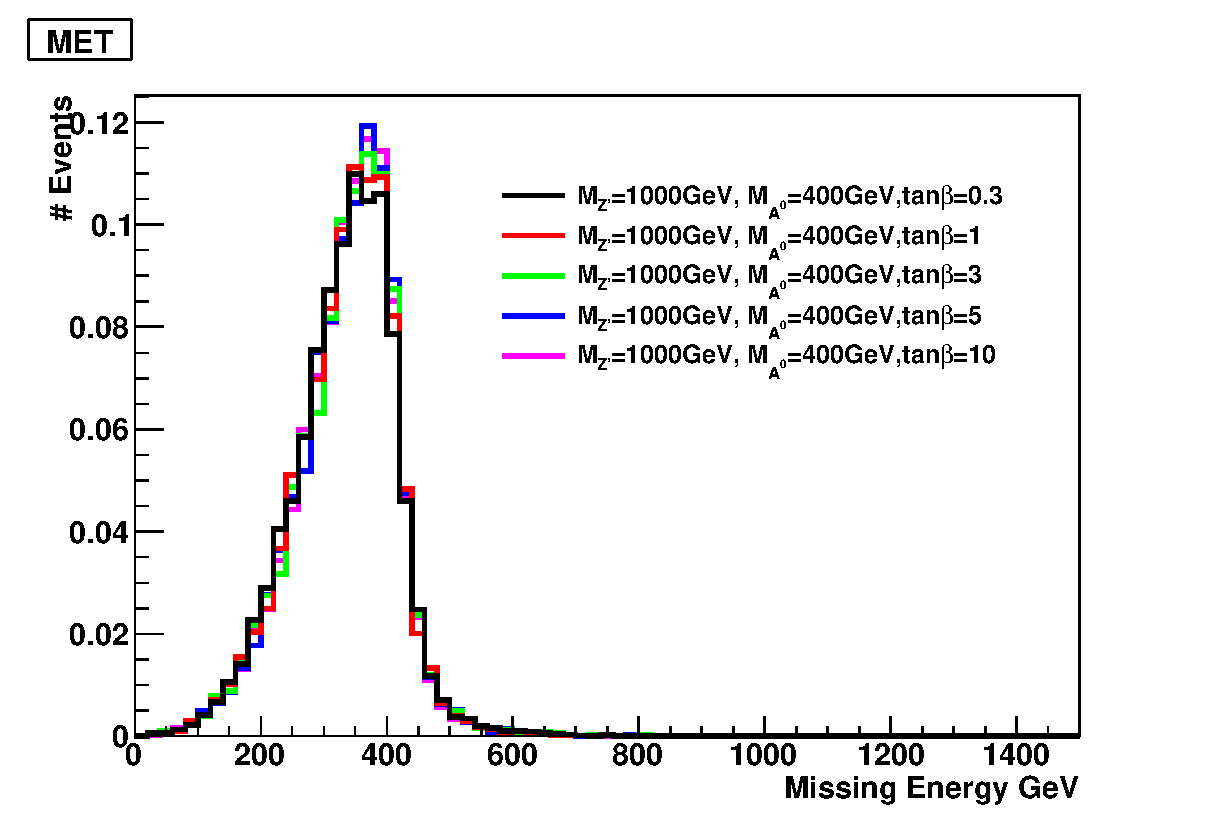
\includegraphics[width=0.75\linewidth]{figures/EW/monoH/2hdm/hxx_zp1000dm10gz01_met}
}
\hfill
\subfloat[$\Delta\phi$ distance between the two $b-$ jets]{
	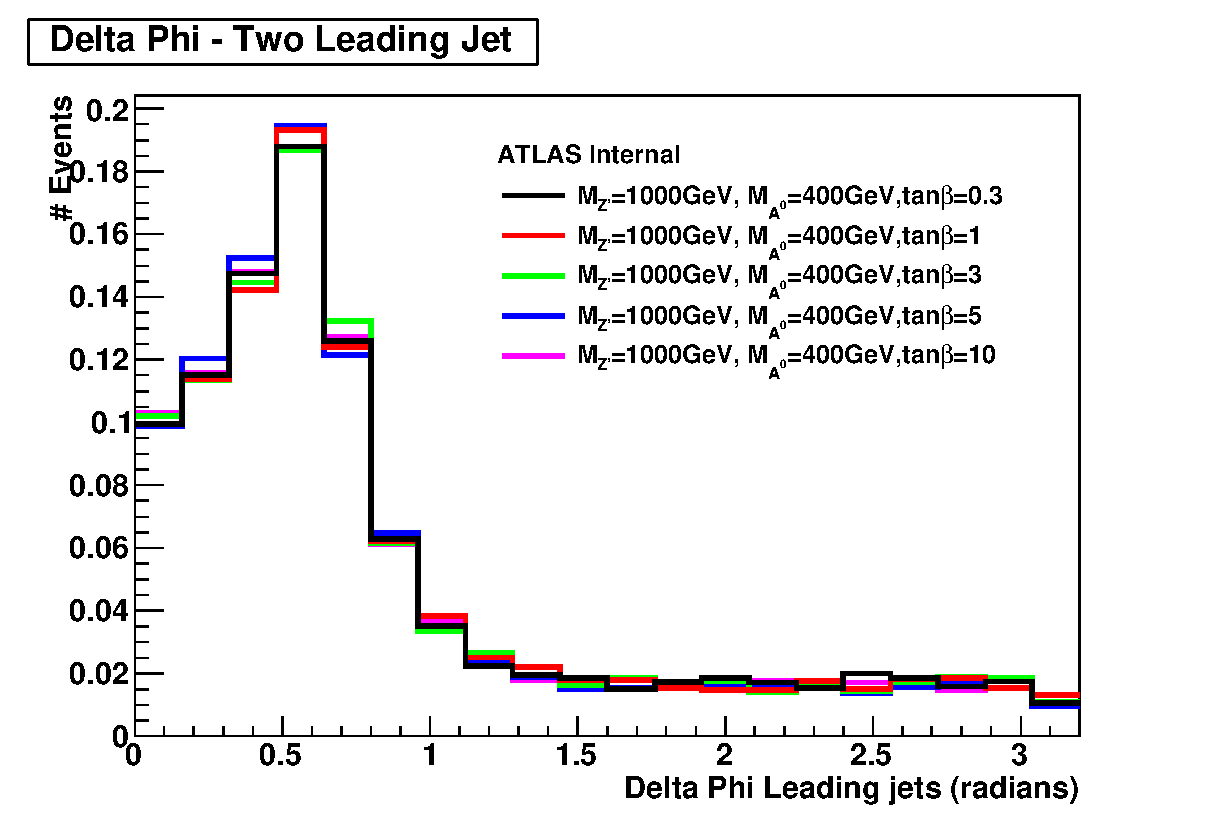
\includegraphics[width=0.75\linewidth]{figures/EW/monoH/2hdm/hxx_zp1000dm10gz01_dphi12}
}
\caption{Kinematic distributions of the signal process varying $\tan{\beta}$, in the case of a Higgs boson decaying into two $b$ quarks,
	after parameterized detector simulation: no kinematic dependence is observed}
\label{fig:DMH_tanbeta}
\end{figure}

Similarly, variations of $g_z$ do not lead to any kinematic changes. 
The value of $g_z$ for a given $M_{\Zprime}$ and $\tan \beta$ can be set according to the maximum value allowed by electroweak global 
fits and dijet constraints, as described in~\cite{Berlin:2014cfa}. Since this parameter does not influence the kinematics, 
we leave it up to individual analyses on whether they generate benchmark points only according to these external constraints.
%\textbf{[TODO: add link to section as in summary. This is the same sentence we will put in for the mono-b model]}.   
%For \Zprime masses below $\sim 1.3$~\tev and larger $\tan \beta$, the $\rho_0$ constraint on $g_z$ is stronger than 
%dijet limits, while for $\tan \beta \lesssim 0.75$,
%the dijet constraints dominate even at low \Zprime masses. 

Since the DM pair are produced as a result of the decay of $A^0$, there are minimal kinematic changes when varying \mDM
as long as $\mDM<M_{A^0}/2$ so that $A^0$ production is on-shell, as shown in Fig.~\ref{fig:DMH_mdm} and~
\ref{fig:zprimeDecay} (before detector simulation). 

\begin{figure}[htpb!]
	\centering
	\subfloat[\MET distribution]{
		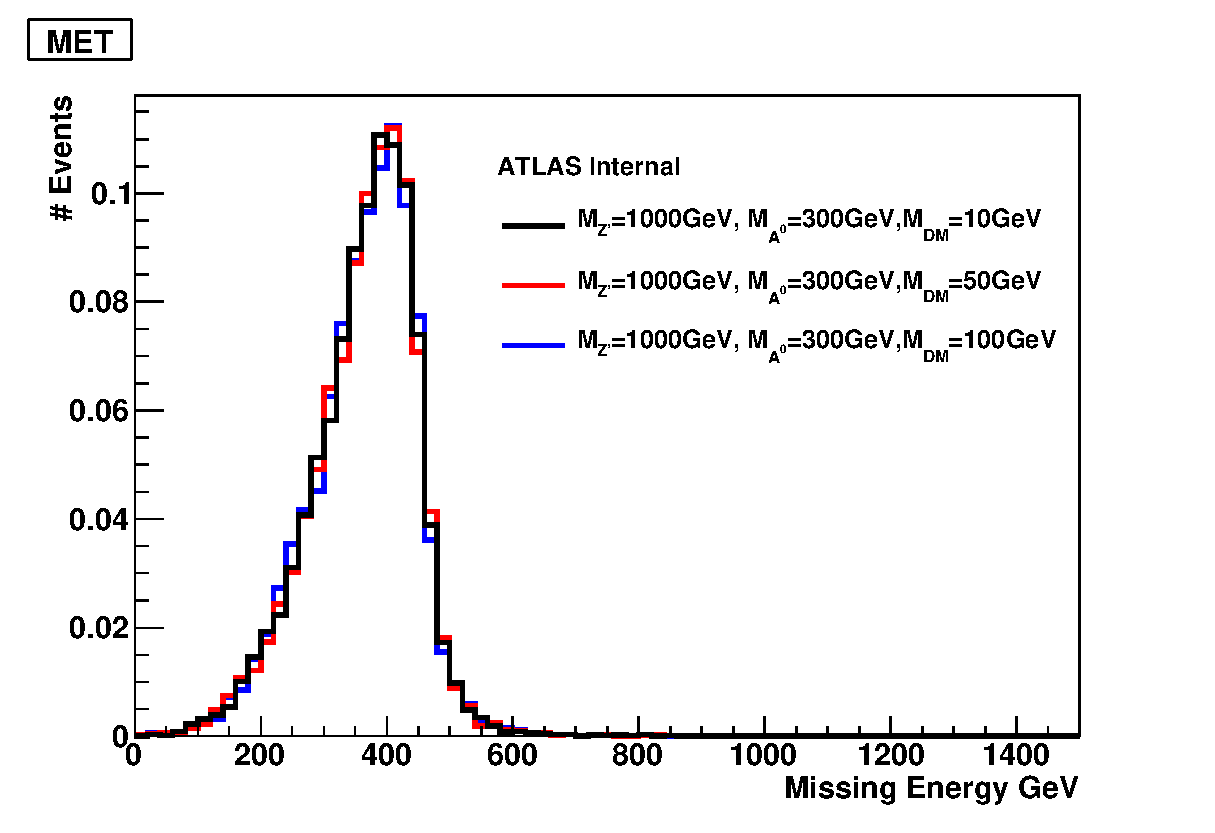
\includegraphics[width=0.75\linewidth]{figures/EW/monoH/2hdm/tanb1zp1000gz08_met}
	}
	\hfill
	\subfloat[$\Delta\phi$ distance between the two $b-$ jets]{
		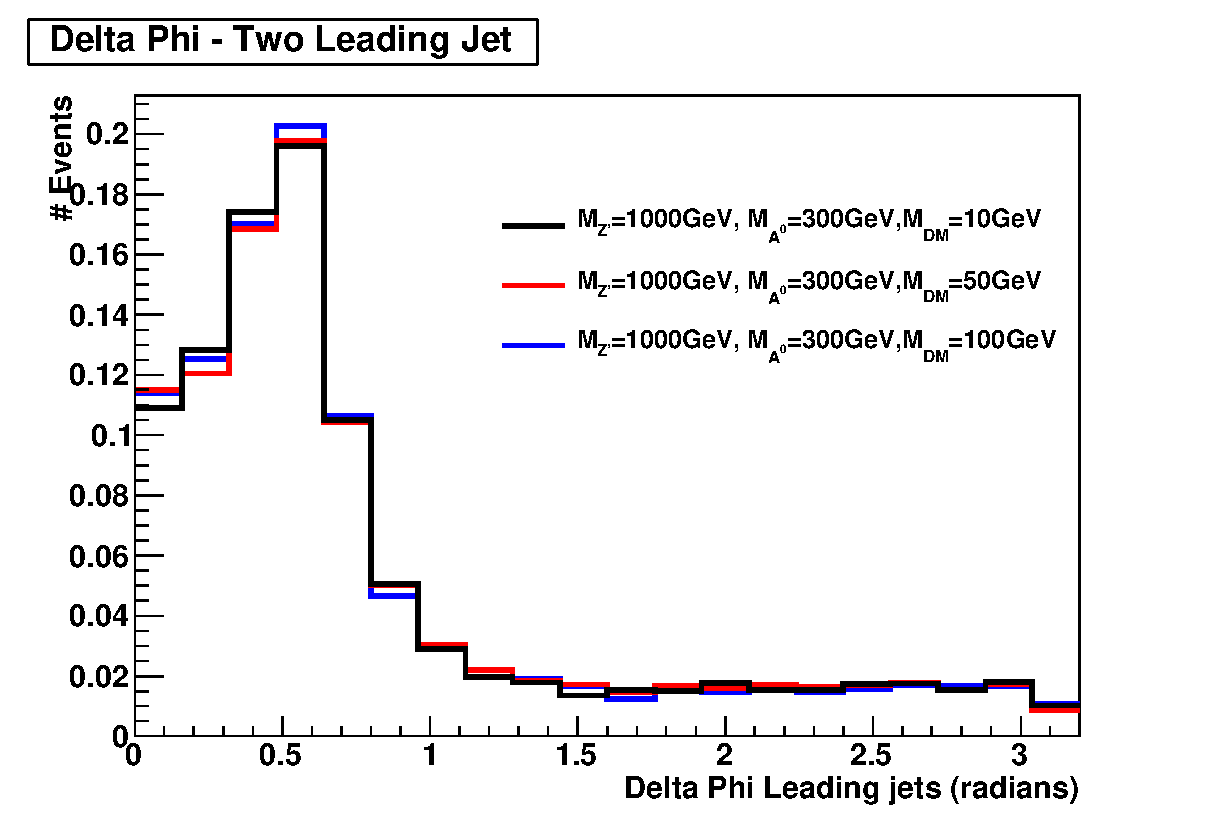
\includegraphics[width=0.75\linewidth]{figures/EW/monoH/2hdm/tanb1zp1000gz08_dphi12}
	}
	\caption{Kinematic distributions of the signal process varying \mDM: minimal kinematic dependency on \mDM as expected when $A^0$ is produced on-shell. Plots shown for $M_{\Zprime}=1000$~\gev, $M_{A^0}=300$~\gev.}
	\label{fig:DMH_mdm}
\end{figure}
 
  \begin{figure}[hbpt!]
  	\centering
  		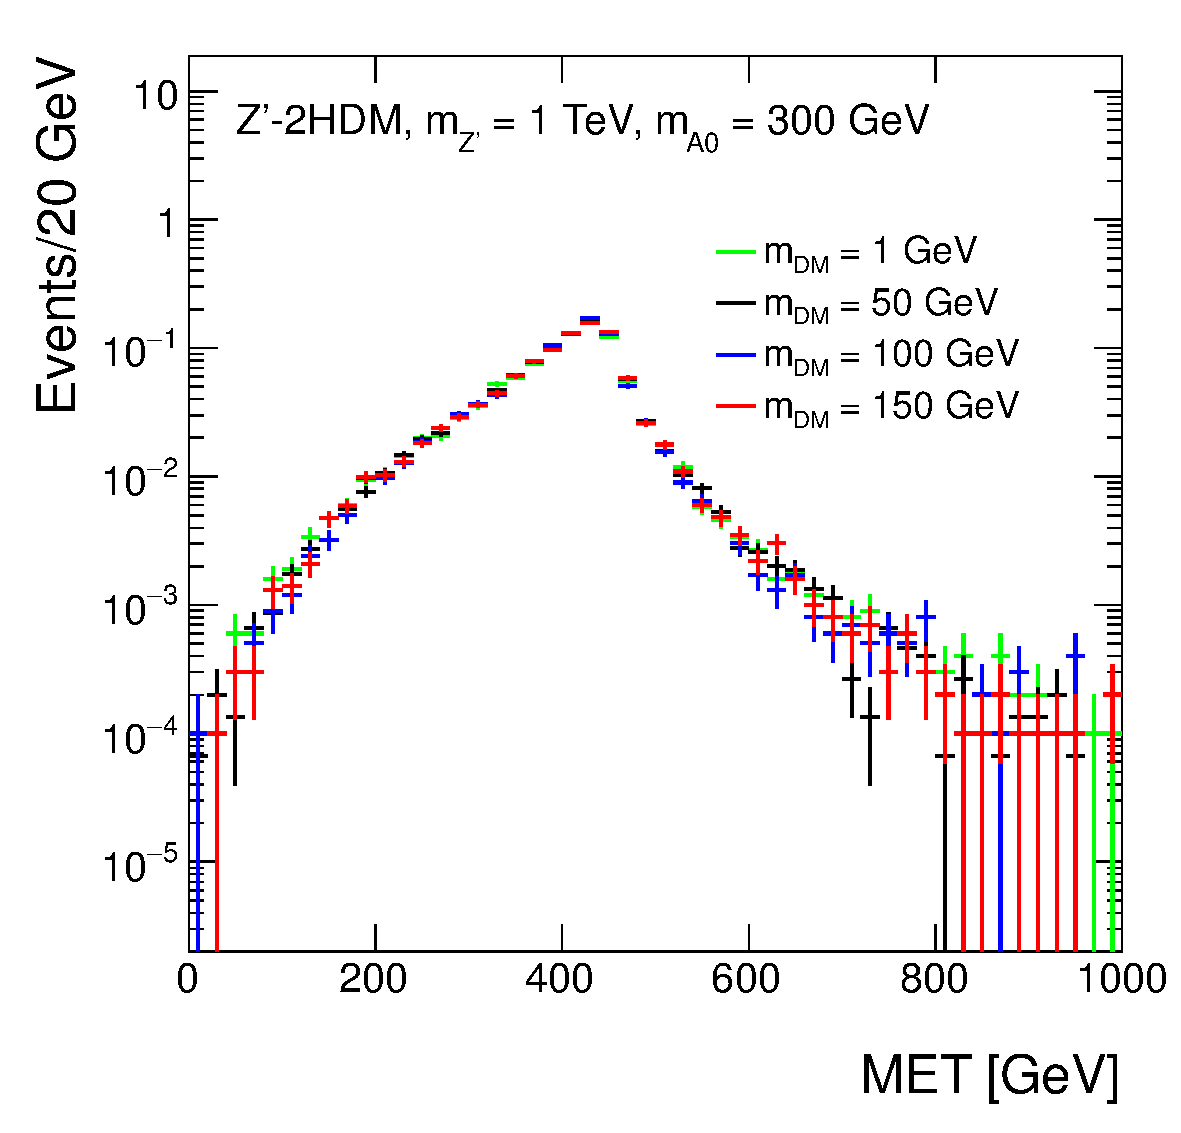
\includegraphics[width=0.75\linewidth]{figures/EW/monoH/zp2hdm_a0_300_MET_et_Log}
  		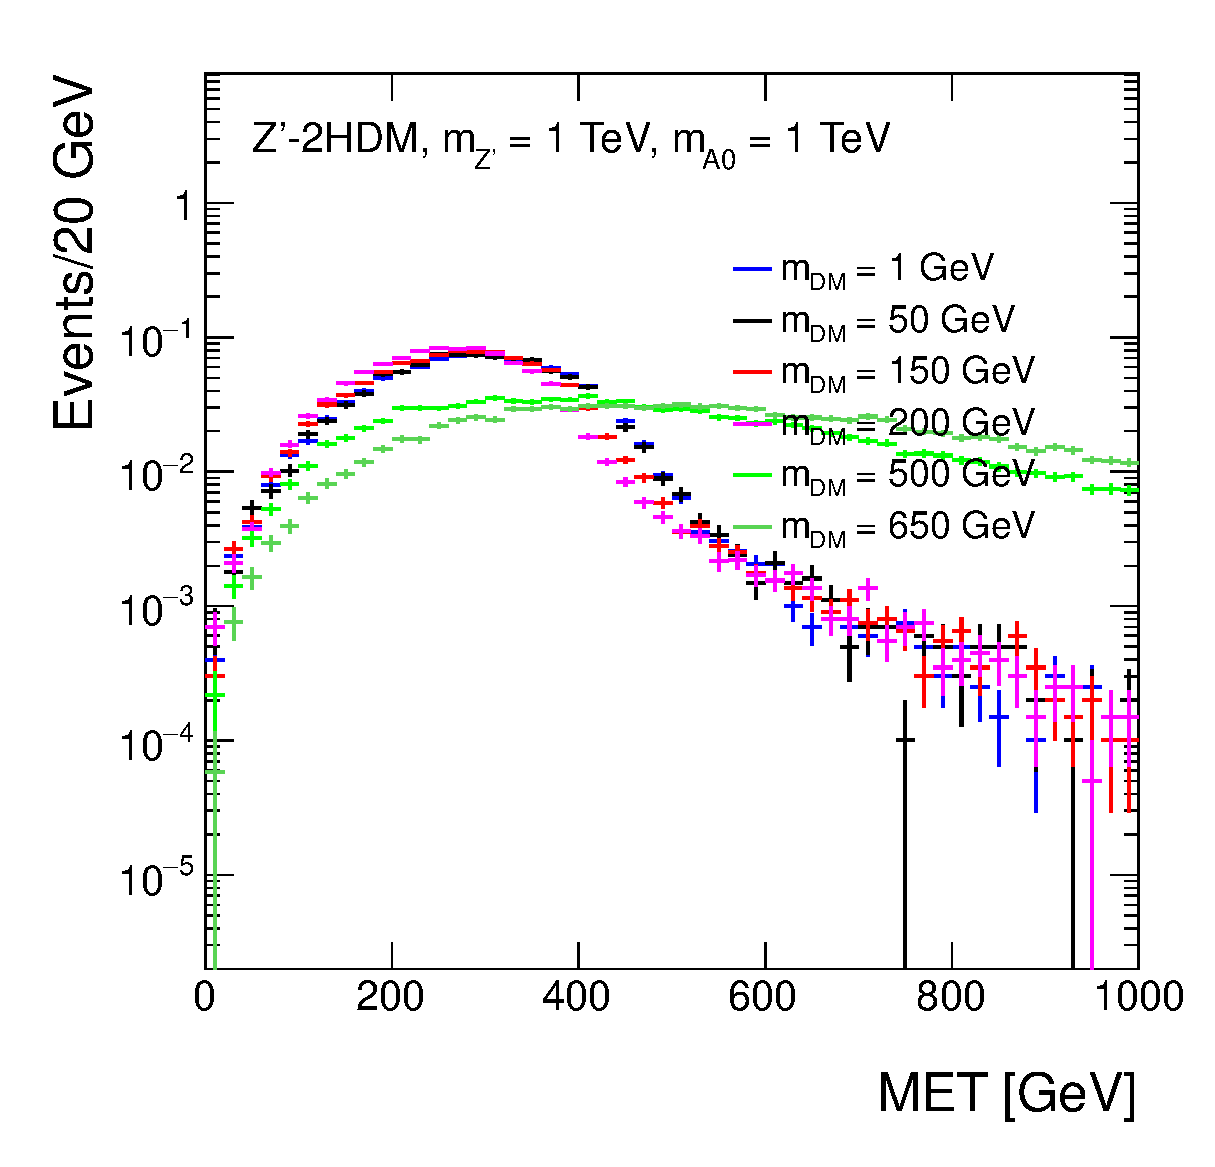
\includegraphics[width=0.75\linewidth]{figures/EW/monoH/zp2hdm_a0_1000_MET_et_Log}
  		\caption{Missing transverse momentum distributions at generator level in the \Zprime+2HDM 
  			scenario for different values of the dark matter mass \mDM, with 
  			$m_{\Zprime}$ = 1~\tev and $m_{A^0}$ = 300~\gev (left) and $m_{A^0}$ = 1~\tev (right).
  			\label{fig:zprimeDecay}}
  \end{figure}
  
We recommend to produce signal events for a fixed $g_z=0.8$, $\tan{\beta}=1$ and $\mDM=100$~\gev. For these values, we scan the 2-D parameter space of ${M_{\Zprime}, M_{A^0}}$ with $M_{\Zprime}=600, 800, 1000, 1200, 1400$~\gev, and $M_{A^0}=300, 400, 500, 600, 700, 800$~\gev with $M_{A^0} < M_{\Zprime}-m_h$, for a total of 24 points. The choice of scan is justified by the sensitivity study in~\cite{Berlin:2014cfa}: the expected LHC sensitivity for Run-2 is up to $M_{\Zprime} \sim 1.5$~\tev.
For the parameter scan, the DM mass is fixed to 100~\gev. For two $M_{\Zprime}$, $M_{A^0}$ value sets, we vary the DM mass to obtain sample cross section for rescaling results. 
All LO cross sections for the various parameter scan points are reported in Appendix~\ref{app:EWSpecificModels_Appendix}.
The parameter scan excludes the off-shell region, as the cross-sections are suppressed and the LHC would not have any
sensitivity to these benchmark points in early data. 

The kinematic distributions with varying $M_{\Zprime}$ for fixed $M_{A^0}$ are shown in Fig.~\ref{fig:DMH_mzp}, while the dependency on $M_{A^0}$ is shown in Fig.~\ref{fig:DMH_ma0}. 
  
 \begin{figure}[htpb!]
 	\centering
 	\subfloat[\MET distribution]{
 		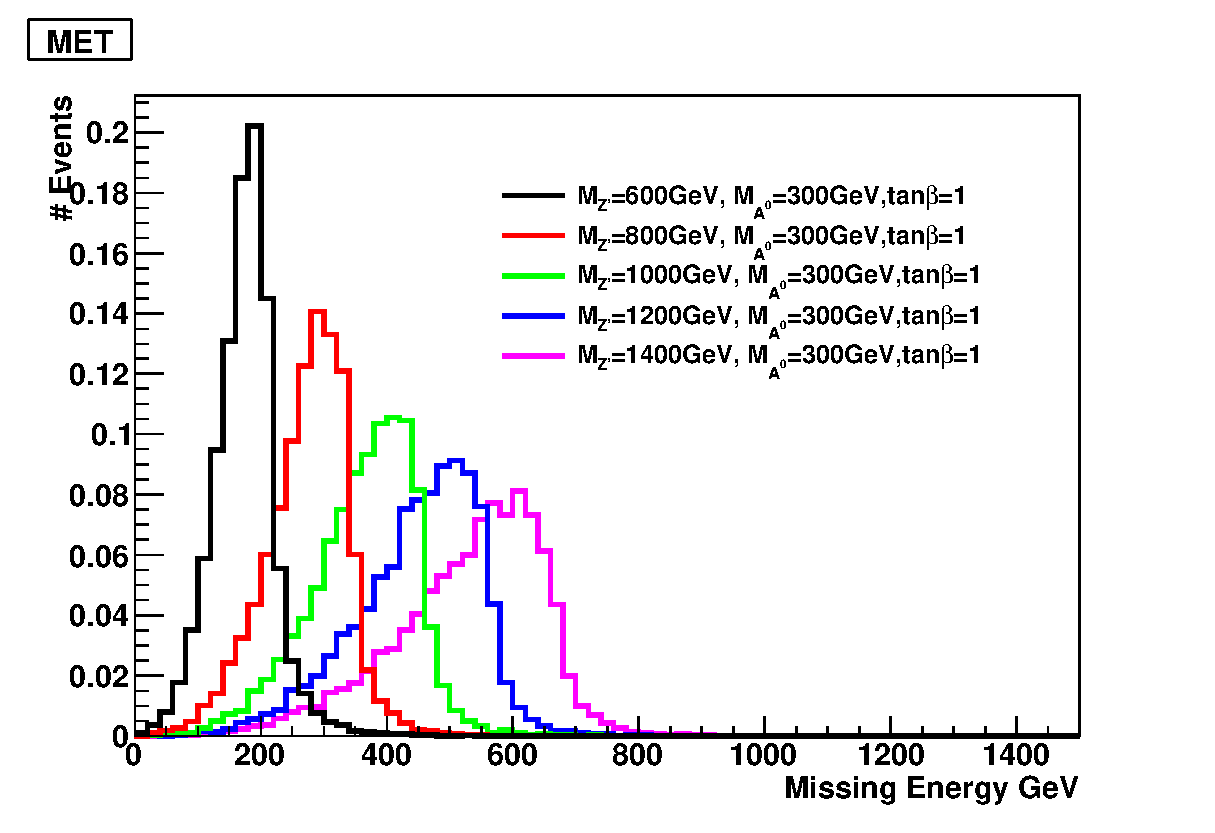
\includegraphics[width=0.8\linewidth]{figures/EW/monoH/2hdm/ZpA0h_tanb1gz08mA300mZp_met}
 	}
 	\hfill
 	\subfloat[Leading $b-$jet $p_T$  distribution]{
 		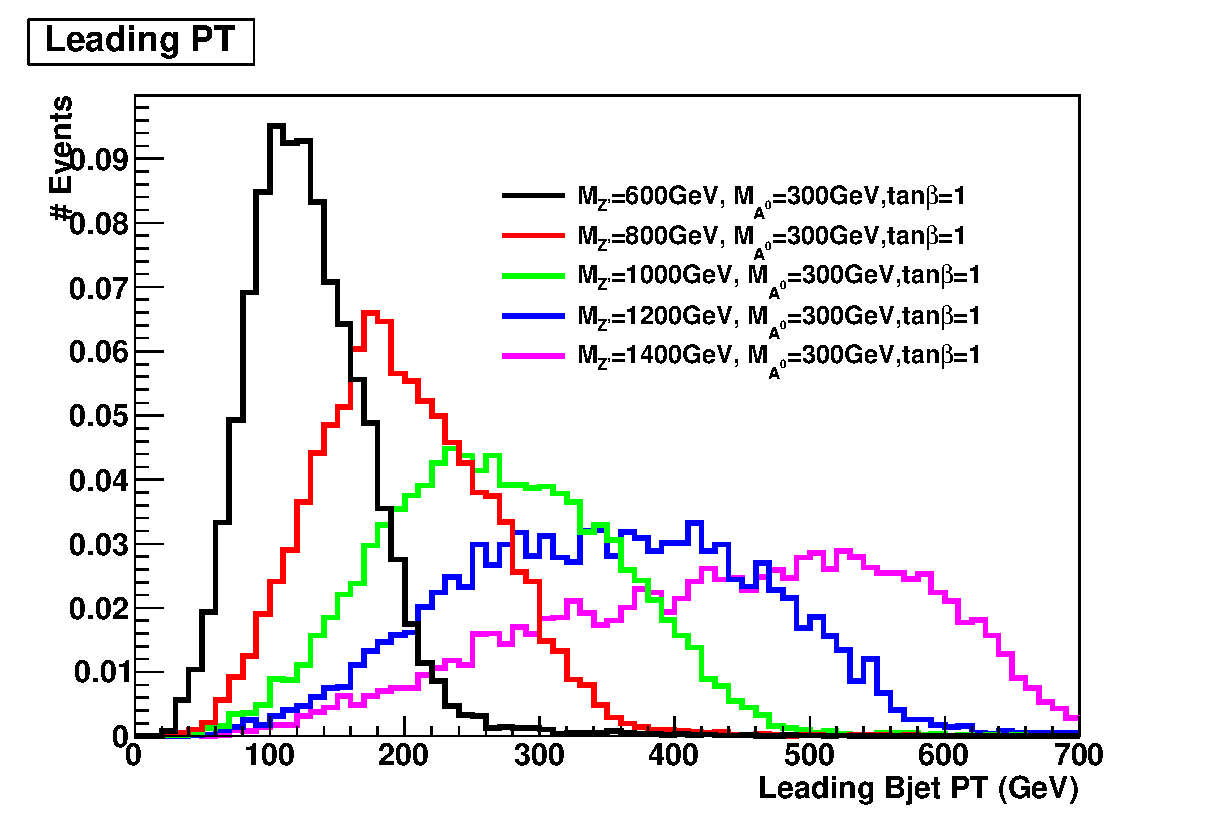
\includegraphics[width=0.8\linewidth]{figures/EW/monoH/2hdm/ZpA0h_tanb1gz08mA300mZp_p0}
 	}
 	\hfill
 	\subfloat[$\Delta\phi$ distance between the two $b-$ jets]{
 		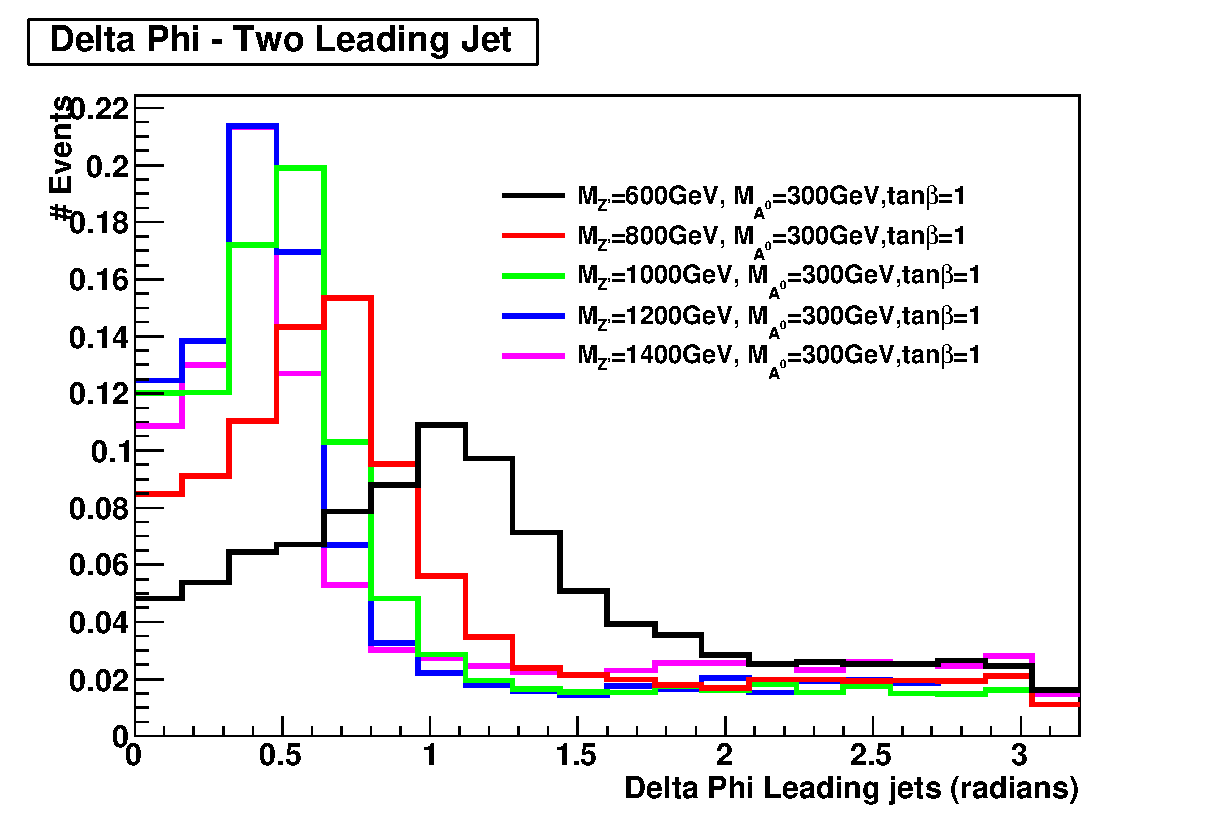
\includegraphics[width=0.8\linewidth]{figures/EW/monoH/2hdm/ZpA0h_tanb1gz08mA300mZp_dphi12}
 	}
% 	\subfloat[Dijet invariant mass]{
% 		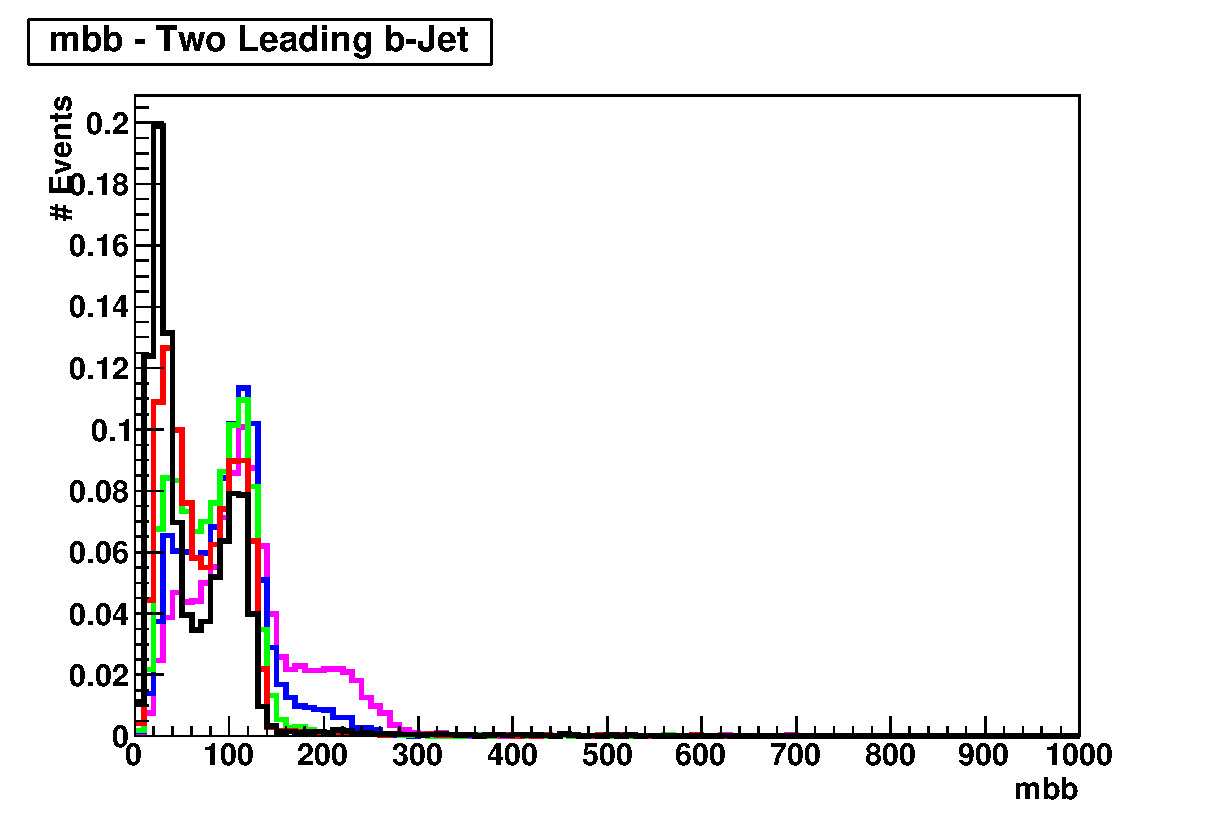
\includegraphics[width=0.75\linewidth]{figures/EW/monoH/2hdm/ZpA0h_tanb1gz08mA300mZp_mbb}
% 	}
 	
 	\caption{Kinematic distributions of the signal process varying $M_{\Zprime}$, for $\mDM=100$~\gev, $M_{A^0}=300$~\gev.}
 	\label{fig:DMH_mzp}
 \end{figure}
  
   \begin{figure}[htpb!]
   	\centering
   	\subfloat[\MET distribution]{
   		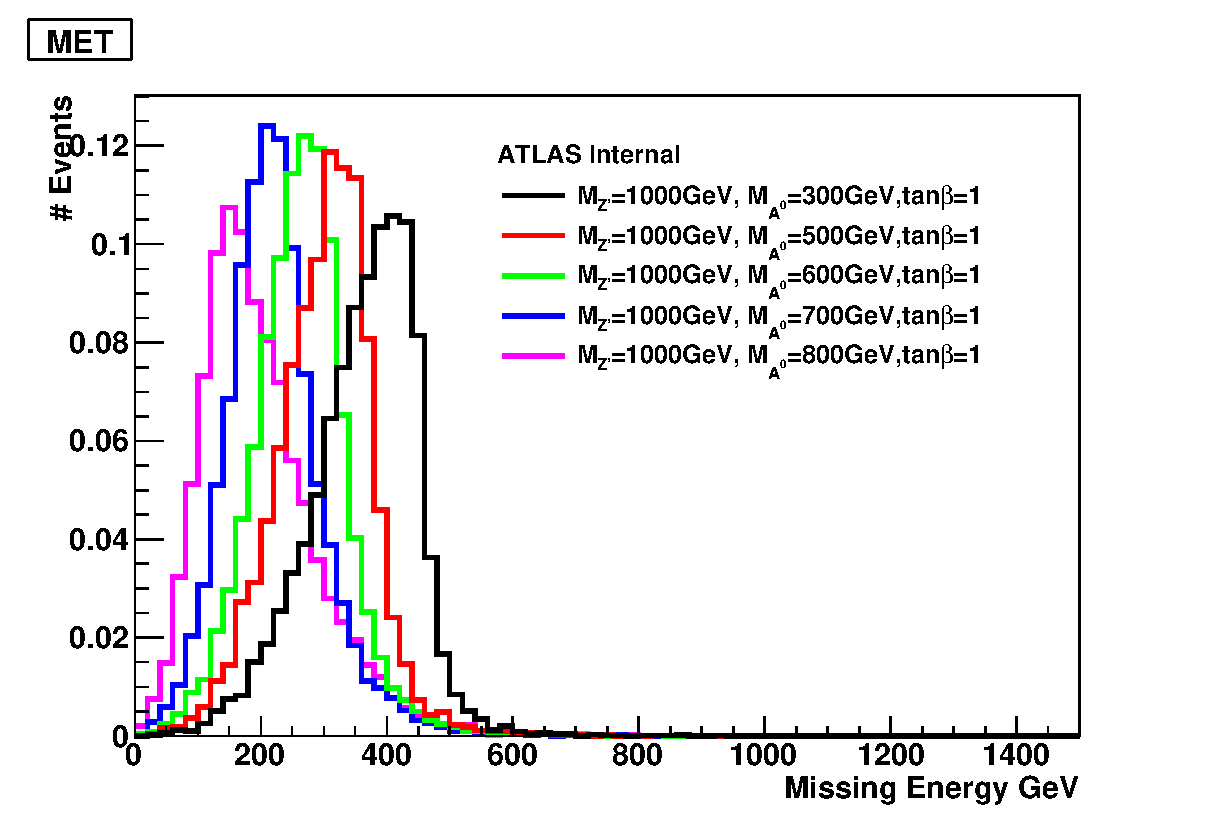
\includegraphics[width=0.8\linewidth]{figures/EW/monoH/2hdm/ZpA0h_tanb1gz08mZp1000mA_met}
   	}\hfill
   	\subfloat[Leading $b-$jet $p_T$ distribution]{
   		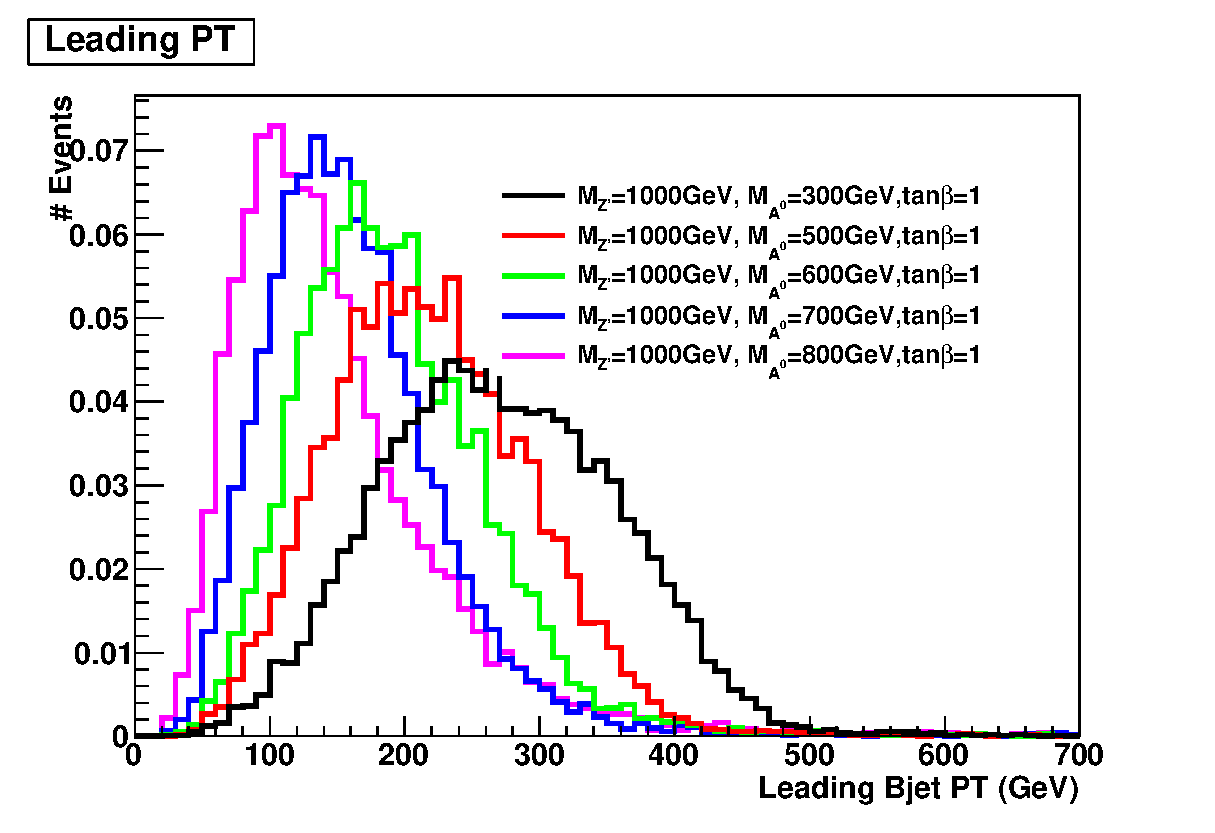
\includegraphics[width=0.8\linewidth]{figures/EW/monoH/2hdm/ZpA0h_tanb1gz08mZp1000mA_p0}
   	}
   	\hfill
   	\subfloat[$\Delta\phi$ distance between the two $b-$ jets]{
   		\includegraphics[width=0.8\linewidth]{figures/EW/monoH/2hdm/ZpA0h_tanb1gz08mZp1000mA_dphi12}
   	}
%   	\subfloat[Dijet invariant mass]{
%   		\includegraphics[width=0.75\linewidth]{figures/EW/monoH/2hdm/ZpA0h_tanb1gz08mZp1000mA_mbb}
%   	}
   	\caption{Kinematic distributions of the signal process varying $M_{A^0}$, for $\mDM=100$~\gev, $M_{\Zprime}=1000$~\gev.}
   	\label{fig:DMH_ma0}
   \end{figure}
      
 This model also allows for an additional source of Higgs plus \MET signal with a similar kinematics (Fig.~\ref{fig:DMH_zpincl}, shown with detector simulation 
 samples) to the signal process from the decay of $\Zprime \to h Z$, where the $Z$ decays invisibly. The partial decay width for the \Zprime is:

 \begin{equation}
 \Gamma_{\Zprime \to hZ}  = (g_z \cos \alpha \sin \beta)^2 \frac{|p|}{24 \pi} \left( \frac{ |p|^2 }{M_{\Zprime}^2} + 3 \frac{M_Z^2}{M_{\Zprime}^2} \right),
 \end{equation}
The values for the \Zprime masses scanned for those samples should follow those of the previous samples, 
namely values of $M_{\Zprime}=600, 800, 1000, 1200, 1400$~\gev.  This signal process has no $M_A$ dependence.
%\Todo{What about visible decays of Z?   And isn't monojet still more sensitive? CD: monojet yes, 
%but for the dijet decays we are asking the same questions for the Z' vector model and I don't think we should worry more here than there.}
 
\begin{figure}[htpb!]
  	\centering
  	\subfloat[\MET distribution]{
  		\includegraphics[width=0.8\linewidth]{figures/EW/monoH/2hdm/Zp_tanb1gz08mA300mZp1000_met}
  	}\hfill
  	\subfloat[Leading $b-$jet $p_T$ distribution]{
  		\includegraphics[width=0.8\linewidth]{figures/EW/monoH/2hdm/Zp_tanb1gz08mA300mZp1000_dphimetj0}
  	}
  	\hfill
  	\subfloat[$\Delta\phi$ distance between the two $b-$ jets]{
  		\includegraphics[width=0.8\linewidth]{figures/EW/monoH/2hdm/Zp_tanb1gz08mA300mZp1000_dphi12}
  	}
%  	\subfloat[Dijet invariant mass]{
%  		\includegraphics[width=0.75\linewidth]{figures/EW/monoH/2hdm/Zp_tanb1gz08mA300mZp1000_mjj}
%  	}
  	\caption{Kinematic distributions of $\Zprime \to A^0\,h$ exclusive production, $\Zprime \to Zh$ exclusive production and \Zprime inclusive production for $M_{\Zprime}=1000$~\gev and $M_{A^0}=300$~\gev}
  	\label{fig:DMH_zpincl}
\end{figure}



  


\section{EFT models with direct DM-boson couplings}
\label{sec:EFT_models_with_direct_DM_boson_couplings}
\svnidlong
{$HeadURL: $}
{$LastChangedDate: $}
{$LastChangedRevision: $}
{$LastChangedBy: $}
\svnid{$Id: $}   

% +++++++++++++++++++++++++++++++++++++++++++++++++++++++++++++++++++++++++++++++++++++
% Linda 11/5/2015
% +++++++++++++++++++++++++++++++++++++++++++++++++++++++++++++++++++++++++++++++++++++

%Despite the appearance of simplified models, we argue that
%the model independent approach of the EFTs is still relevant.
The EFT operators considered in this section do not have an implementation 
of a simplified model completion for Dirac fermion Dark Matter available to date. 
They provide kinematic distributions that 
are unique to mono-boson signatures, and that in most cases 
are not reproduced by an equivalent simplified model.\sidenote{Wherever this is
the case, for practical reasons one can only generation a simplified model result 
in the limiting EFT case, as the results can be rescaled and reinterpreted.}

A complete list of effective operators with direct DM/boson couplings for
Dirac DM, up to dimension 7, can be found in~\cite{Cotta:2012nj, Carpenter:2012rg, Crivellin:2015wva}. 
Higher dimensional operators, up to dimension 8, leading to Higgs+\MET signatures,
are mentioned in~\cite{Carpenter:2012rg, Berlin:2014cfa}. The first part of this Section outlines
the main characteristics for a limited number of these models that could be 
considered in early Run-2 searches. 
However, the EFT approximation made for these operators can be problematic, see Ref.~\cite{Berlin:2014cfa} for discussion.
For this reason, model-independent results as in Appendix~\ref{app:Presentation_Of_Experimental_Results} 
should be privileged over considering these operators as realistic benchmarks. 
%We also recommend not to optimize searches based on those benchmark models. 

However, the Forum discussion highlighted that the EFT approach allows
more model-independence when reinterpreting results, and that it is worth still considering
interpretation of the results available in terms of these operators. Furthermore, once simplified models are available
for those operators, EFT results can be used as a limiting case for consistency checks. 
We devote the end of this Section to a discussion on the presentation of results 
from this model, including an assessment of their reliability 
using a conservative procedure that is only dependent on EFT parameters.

The studies in this Section
have been performed using a UFO model within \madgraph v2.2.3, interfaced to \pythia 8 for the parton shower.  
The implementation of these models is discussed further in Section~\ref{sub:EFTModels}.

%CD: what is this?
%\newthought{Implementation discussed in the Appendix}

%%%%%%%%%%%Dimension 5 operators
\subsection{Dimension 5 operators}
\label{sub:EW_EFT_Dim5}

The lowest dimension benchmark operators we consider are effective dimension 5,
such as the one depicted in Figure~\ref{fig:modelMonoHEFT}.  

\begin{figure}[!htb]
	\centering
	\unitlength=0.005\textwidth
    \vspace{3\baselineskip}
	\begin{feynmandiagram}[modelMonoHEFT]
		\fmfleft{i1,i2}
		\fmfright{o1,o2,ohidden,o3}
		\fmf{fermion}{i2,v1,i1}
		\fmflabel{\Large $q,g$}{i2}
		\fmflabel{\Large $\bar{q},g$}{i1}
		\fmf{dashes}{v1,v2}
		\fmfv{decor.shape=circle,decor.filled=shaded, decor.size=30,label={\Large $\text{EFT}(\lambda,,\Lambda)$},label.a=30,label.d=15}{v2}
		\fmf{dashes}{v2,o3}
		\fmflabel{\Large $h$}{o3}
		\fmf{fermion}{o2,v2,o1}
		\fmflabel{\Large ${\bar{\chiDM}}$}{o1}
		\fmflabel{\Large ${\chiDM}$}{o2}
		\fmfdot{v1}
	\end{feynmandiagram}
    \vspace{3\baselineskip}
	\caption{Diagram for EFT operators giving rise to a Higgs+\MET signature.}
	\label{fig:modelMonoHEFT}
\end{figure}

Following the notation of~\cite{Carpenter:2012rg},  models
from this category have a Lagrangian that, after electroweak symmetry breaking, 
includes terms such as:

\begin{eqnarray}
\frac{m_W^2}{\Lambda_5^3} ~\bar{\chiDM} \chiDM ~W^{+ \mu} W^{-}_\mu
+ \frac{m_Z^2}{2 \Lambda_5^3} ~ \bar{\chiDM} \chiDM ~ Z^\mu Z_\mu ~,
\end{eqnarray}
where $m_Z$ and $m_W$ are the masses of the $Z$ and $W$ boson, $W^{\mu}$ and $Z^{\mu}$
are the fields of the gauge bosons, $\chiDM$ denotes the Dark Matter fields
and $\Lambda_5$ is the effective field theory scale. Note that these operators are of true dimension 7, 
but reduce to effective dimension 5 once the Higgs vacuum expectation values, 
contained in the W and Z mass terms, are inserted.  
As such, one expects that these operators would naturally arise in UV complete models where Dark Matter 
interacts via a Higgs portal where heavy mediators couple to the Higgs or other fields in an extended Higgs sector. 
In such models the full theory may be expected to contain additional operators with Higgs-Dark Matter couplings~\cite{Djouadi:2012zc}.
The above operator also induces signatures with 
\MET in conjunction with Z and W bosons at tree level, as shown in Fig.~\ref{fig:VPlusMET_EFT},
while at loop level it induces couplings to photon pairs and $Z \gamma$ through W loops.
In these models, a clear relation exists between final states with photons, EW bosons
and Higgs boson. 

As shown in Fig.~\ref{fig:EW_EFT5_Zlep_MET}, the 
kinematics of this model can be approximated by that of a simplified model including 
a high-mass scalar mediator exchanged in the \schannel described in Section~\ref{sub:EW_Scalar}. 
For this reason, the list of benchmark models with direct boson-DM couplings for photon, Z and W 
only includes dimension 7 operators: if the scalar model with initial state radiation of an EW boson
is already generated, then its results can be rescaled. 

The Higgs+\MET analysis,
however, will not consider the scalar simplified model as benchmark, due to the very low sensitivity 
in early LHC analyses, and will instead use this dimension 5 operator. 

\begin{figure}
	\includegraphics[width=0.95\textwidth]{figures/EW/pt_vv2_xxDHDH_vs_ScalarMediator.pdf}
	\caption{Comparison of the missing transverse momentum for the simplified model
		where a scalar mediator is exchanged in the \schannel and the model including 
		a dimension-5 scalar contact operator, in the leptonic Z+\MET final state. All figures in this Section
		have been performed using a UFO model within \madgraph v2.2.3, interfaced to \pythiaEight for the parton shower.  }
	\label{fig:EW_EFT5_Zlep_MET}
\end{figure}

\subsubsection{Parameter scan}

The two parameters of this model are the scale of new physics $\lambda$ 
and the DM particle mass. SM-DM coupling and new physics scale are related by 
$\gDM = {(246~\gev)}/{\lambda}$. 


The initial value of the new physics scale $\lambda$ chosen 
for the sample generation is 3~\tev. This is a convention and does not affect the signal kinematics:
the cross-section of the samples can be rescaled when deriving the constraints on this scale. 
However, more care should be given when rescaling Higgs+\MET operators
of higher dimensions, as different diagrams have a different $\lambda$ dependence. 
%From Andy
%– Lambda=3~\tev. Essentially this is an arbitrary choice for most EFTs, 
%however it does affect the mono-H analysis as some of their models 
%have non-trivial scaling with Λ. More care should be given to the choice for mono-H. 

The DM mass values for the benchmark points to be simulated are chosen to
span a sufficient range leading to different kinematics, 
that is within the LHC sensitivity for early searches and that is consistent across 
the various signatures and EFT operators. We therefore start the mass scan
at \mdm=1~\gev, where collider experiments are complementary to direct and indirect detection
and choose the last point corresponding to a DM mass of 1~\tev. 
We recommend a scan in seven mass points, namely:
$$
\mdm = { 1, 10, 50, 100, 200, 400, 800, 1300 } \gev. 	
$$

A set of kinematic distributions from the Higgs+\MET signature where the Higgs decays 
into two $b-$quarks is shown in Fig.~\ref{fig:Hbb_Dim5}, for points similar to those of the grid scan proposed. 
  
 \begin{figure}[hbpt!]
 	\centering
 	\subfloat[Leading $b-$jet transverse momentum]{
 		\includegraphics[width=0.8\linewidth]{figures/EW/monoH/xxhhg5/truth_leading_b_pt} %\label{fig:met_cmp_high}
 	}
 	\hfill
 	\subfloat[Leading $b-$jet pseudorapidity]{
 		\includegraphics[width=0.8\linewidth]{figures/EW/monoH/xxhhg5/truth_leading_b_eta} %\label{fig:met_cmp_low}
 	}
 	\hfill
% 	\subfloat[Leading $b-$jet transverse momentum]{
% 		\includegraphics[width=0.95\linewidth]{figures/EW/monoH/xxhhg5/truth_subleading_b_pt} %\label{fig:met_cmp_high}
% 	}
% 	\hfill
% 	\subfloat[Leading $b-$jet pseudorapidity]{
% 		\includegraphics[width=0.95\linewidth]{figures/EW/monoH/xxhhg5/truth_subleading_b_eta} %\label{fig:met_cmp_low}
% 	}
% 	\hfill

 	\subfloat[Angular distance between the two leading $b-$jets]{
 		\includegraphics[width=0.8\linewidth]{figures/EW/monoH/xxhhg5/truth_bb_deltar} %\label{fig:met_cmp_low}
 	}
 	\caption{Comparison of the kinematic distributions for the two leading $b-$ jets (from the Higgs decay) in the model with direct interactions
 		between the Higgs boson and the DM particle, when varying the DM mass. 
 		\label{fig:Hbb_Dim5}}
 \end{figure}
 
 
%%%%%%%%%%%%%Dimension 7 operators

\subsection{Dimension 7 operators}
\label{sub:EW_EFT_Dim7}

% +++++++++++++++++++++++++++++++++++++++++++++++++++++++++++++++++++++++++++++++++++++
% Uli 3/5/2015
% +++++++++++++++++++++++++++++++++++++++++++++++++++++++++++++++++++++++++++++++++++++

The dimension-7 benchmark models  contain the $SU(2)_L \times U(1)_Y$ gauge-invariant couplings between 
DM fields and the kinetic terms of the EW bosons. The CP-conserving scalar couplings of this type can be written as
\begin{equation} \label{eq:Lc1c2}
\frac{c_1}{\Lambda_S^3} \, \bar \chiDM \chiDM \, B_{\mu \nu} B^{\mu \nu }  + \frac{c_2}{\Lambda_S^3} \, \bar \chiDM \chiDM \, W_{\mu \nu}^i W^{i, \mu \nu }  \,.
\end{equation}
Here $B_{\mu \nu} = \partial_\mu B_\nu - \partial_\nu B_\mu$ and $W_{\mu \nu}^i =  \partial_\mu W_\nu^i - \partial_\nu W_\mu^i + g_2 \hspace{0.25mm} \epsilon^{ijk}  \hspace{0.25mm}  W_\mu^j \hspace{0.25mm} W_\mu^k$ are the $U(1)_Y$ and $SU(2)_L$ field strength tensor, respectively, and  $g_2$ denotes the weak coupling constant. In the case of the pseudoscalar couplings, one has instead
\begin{equation} \label{eq:Lc3c4}
\frac{c_1}{\Lambda_P^3} \, \bar \chiDM \gamma_5 \chiDM \, B_{\mu \nu} \tilde B^{\mu \nu }  + \frac{c_2}{\Lambda_P^3} \, \bar \chiDM \gamma_5 \chiDM \, W_{\mu \nu}^i \tilde W^{i, \mu \nu }  \,,
\end{equation}
where $\tilde B_{\mu \nu} = 1/2 \hspace{0.5mm} \epsilon_{\mu \nu  \lambda \rho}  \hspace{0.25mm}  B^{\lambda \rho}$ and $\tilde W_{\mu \nu}^i = 1/2 \hspace{0.5mm} \epsilon_{\mu \nu  \lambda \rho}  \hspace{0.25mm}  W^{i, \lambda \rho}$ are the dual  field strength tensors. In addition to the CP-conserving interactions (\ref{eq:Lc1c2}) and (\ref{eq:Lc3c4}), there are also four CP-violating couplings that are obtained from the above operators by the replacement $\bar \chiDM \chiDM \leftrightarrow \bar \chiDM \gamma_5 \chiDM$.

The effective interactions introduced in (\ref{eq:Lc1c2}) and  (\ref{eq:Lc3c4}) appear  in models of Rayleigh DM~\cite{Weiner:2012cb}. Ultraviolet completions where the operators are generated through loops of states charged under $U(1)_Y$ and/or $SU(2)_L$  have been proposed in \cite{Weiner:2012gm} and their LHC signatures have been studied in \cite{Liu:2013gba}. If these new charged particles  are  light, the high-$p_T$ gauge bosons that participate in  the \MET processes considered here are able to resolve the substructure of the loops. This generically suppresses the cross sections compared to the EFT predictions~\cite{Haisch:2012kf}, and thus will weaken the bounds on the interaction strengths of  DM and the EW gauge bosons  to some extent.  Furthermore, the light charged mediators may be produced  on-shell in $pp$ collisions, rendering direct LHC searches potentially more restrictive than \MET searches. Making the above statements precise would require further studies beyond the timescale of this forum.

Since for $\Lambda_S = \Lambda_P$ the effective interactions (\ref{eq:Lc1c2}) and (\ref{eq:Lc3c4}) predict essentially the same value of the mono-photon, mono-$Z$ and mono-$W$ cross section \cite{Carpenter:2012rg,Crivellin:2015wva}, we consider below only the former couplings. We emphasize however that measurements of the jet-jet azimuthal angle difference in \MET$+ 2 j$ events may be used to disentangle whether DM couples more strongly to the combination $B_{\mu \nu} B^{\mu \nu}$ ($W_{\mu \nu}^i W^{i, \mu \nu }$) or the product $B_{\mu \nu} \tilde B^{\mu \nu}$ ($W_{\mu \nu}^i \tilde W^{i, \mu \nu }$) of field strength tensors \cite{Cotta:2012nj,Crivellin:2015wva}.

After EW symmetry breaking the interactions (\ref{eq:Lc1c2}) induce direct couplings 
between pairs of DM particles and  gauge bosons.  The corresponding Feynman rule reads:

\begin{equation}  \label{eq:feynman}
\frac{4 \hspace{0.25mm} i}{\Lambda_S^3} \; g_{V_1 V_2} \, \big (  p_1^{\mu_2} \hspace{0.25mm} p_2^{\mu_1} - g^{\mu_1 \mu_2}  \, p_1 \cdot p_2 \big ) \,,
\end{equation}
where $p_i$ ($\mu_i$) denotes the momentum (Lorentz index) of the vector field $V_i$ and for simplicity the spinors associated with the DM fields have been dropped. The couplings $g_{V_i V_j}$ take the form:

\begin{equation} \label{eq:gViVj}
\begin{split}
g_{\gamma \gamma} & = c_w^2 \hspace{0.25mm} c_1+ s_w^2  \hspace{0.25mm} c_2 \,, \\[1mm]
g_{\gamma Z}   & = - s_w c_w \, \big (  c_1  - c_2  \big ) \,, \\[1mm]
g_{ZZ}  & = s_w^2 \hspace{0.25mm} c_1 + c_w^2  \hspace{0.25mm} c_2  \,, \\[1mm]
g_{WW} & = c_2 \,,
\end{split}
\end{equation}
with $s_w$ ($c_w$) the sine (cosine) of the weak mixing angle. Note that our coefficients $c_1$ and $c_2$ are identical to the coefficients $C_B$ and $C_W$ used in \cite{Crivellin:2015wva}, while they are related via $k_1 = {c_w}^2 c_1$ and $k_2 = {s_w}^2 c_2$ to the coefficients $k_1$ and $k_2$ introduced in \cite{Carpenter:2012rg}.

%Uli:
%the couplings k_1,2 "defined"  there agree with my c_1,2 if one identifies
%
%k_1 = c_W^2 c_1
%
%k_2 = s_W^2 c_2

The coefficients $c_1$ and $c_2$ appearing in (\ref{eq:gViVj}) determine the relative importance of each of the \MET channels and their correlations. For example, one observes that:
\begin{itemize}
 \item Only $c_2$ enters the coupling between DM and $W$ bosons, meaning that only models with $c_2 \neq 0$ predict a mono-$W$ signal;
 \item If $c_1 = c_2$ the mono-photon (mono-$Z$) signal does not receive contributions from diagrams involving $Z$ (photon) exchange;
  \item Since numerically $c_w^2/s_w^2 \simeq 3.3$ the mono-photon channel is particularly sensitive to $c_1$.
\end{itemize}

% +++++++++++++++++++++++++++++++++++++++++++++++++++++++++++++++++++++++++++++++++++++
% +++++++++++++++++++++++++++++++++++++++++++++++++++++++++++++++++++++++++++++++++++++
\subsubsection{Parameter scan}

As stated above and shown in Ref.~\cite{Nelson:2013pqa}, 
the kinematic distributions for dimension-7 scalar and pseudoscalar operators
only shows small differences. This has been verified from a generator-level study:
the signal acceptance after a simplified analysis selection 
(\MET$>$350~\gev, leading jet $p_T > $ 40~\gev, minimum azimuthal difference between
either of the two jets and the \MET direction $>$ 0.4) is roughly 70\% for both models, independent from the coefficients $c_1$ and $c_2$. 
We therefore only suggest to generate one of the two models.
%Todo{When we have the cross-sections for both, we can recommend the one with the highest cross-section.}

%as shown in Fig.~\ref{fig:EW_EFT5_gamma_MET}.
%\begin{figure}
%    \includegraphics[width=0.6\textwidth]{figures/llug}
%    \caption{Comparison of the missing transverse momentum for the scalar and pseudoscalar
%    operators with direct interaction between DM and photon, in the photon+\MET final state}
%    \label{fig:EW_EFT5_gamma_MET}
%\end{figure}

The differences in kinematics for the various signatures
are negligible when changing the coefficients $c_1$ and $c_2$, 
since these coefficient factorize in the matrix element. 
Only the case $c_1=c_2=1$ is generated as benchmark;
other cases are left for reinterpretation as they will only need a 
rescaling of the cross-sections. 
%\Todo{Appendix~\ref{app:EWSpecificModels_Appendix} contains cross-sections
%	for these operators, for values }
%for the various DM
%mass points considered.

\begin{figure}[h!]
  \centering
%  \subfloat[Missing transverse momentum distribution.\label{fig:EFTD7_EW_Z_MET}]{%
  	\includegraphics[width=0.95\textwidth]{figures/EW/monoZhad_SP/metPt}
%  }
%  \hfill
%  \subfloat[Acceptance.\label{fig:EFTD7_EW_Z_acc}]{%
%  	\includegraphics[width=0.7\textwidth]{figures/EW/monoZhad_SP/Sscale_newplot.pdf}
%  }
    \caption{\MET distribution for the dimension-7 model with a hadronically decaying Z in the final state,
    for the scalar and pseudoscalar operators representing direct interactions between DM and bosons. The values of the coefficients in the legend are multiplied by 100.}
    \label{fig:EFTD7_EW_kinematics}
\end{figure}


%%%%%%%%%%%%%Dimension 8 operators

\subsection{Higher dimensional operators}

Many higher dimensional operators can induce signals of photons or $W/Z/H$ bosons
in the final state. A complete list can be found in Refs.~\cite{Carpenter:2013xra, Berlin:2014cfa, Petrov:2013nia}
and references therein. 

Although with lower priority with respect to the operators above, 
a representative dimension-8 operators can be chosen as benchmark, with the form:
 
$$\frac{1}{\Lambda^4} \bar{\chiDM} \gamma^{\mu} \chiDM B_{\mu \nu} H^{\dagger} D^{\nu} H$$

In this case, the new physics scale is $\Lambda$ is connected with the coupling
of the DM as $\displaystyle y_{\chiDM} = \frac{1}{\Lambda^{4}}$.\Todo{Is more detail needed here?}
An advantage of this operator is that it includes all signatures with EW bosons,
allowing to assess the relative sensitivity of the various channels with the same model.  
The kinematics for this operator is different with respect to other operators,
leading to a harder \MET spectrum, 
as illustrated by comparing the leading $b-$jet distribution for the dimension 5 operator
to the dimension 8 operator. 
  
   \begin{figure}[hbpt!]
   	\centering
   	\subfloat[Dimension 5 operator]{
   		\includegraphics[width=0.95\linewidth]{figures/EW/monoH/xxhhg5/truth_leading_b_pt} %\label{fig:met_cmp_high}
   	}
   	\hfill
   	\subfloat[Dimension 7 operator]{
   		\includegraphics[width=0.95\linewidth]{figures/EW/monoH/xgxFhDh/truth_leading_b_pt} %\label{fig:met_cmp_high}
   	}
   	\caption{Comparison of the transverse momentum for the leading $b-$ jet from the Higgs decay for a dimension 5 and dimension 7 operator
   		with direct boson-DM couplings.}
   	\end{figure}
  

%\subsection{xgxFhDh Truth Kinematics}
%
%\begin{figure}[!htbp]
%	\begin{minipage}{0.5\textwidth}
%		\centering
%		\includegraphics[width = \linewidth]{xgxFhDh/truth_leading_b_pt.eps}
%	\end{minipage}
%	\begin{minipage}{0.5\textwidth}
%		\centering
%		\includegraphics[width = \linewidth]{xgxFhDh/truth_leading_b_eta.eps}
%	\end{minipage}
%\end{figure}
%
%\begin{figure}[!htbp]
%	\begin{minipage}{0.5\textwidth}
%		\centering
%		\includegraphics[width = \linewidth]{xgxFhDh/truth_subleading_b_pt.eps}
%	\end{minipage}
%	\begin{minipage}{0.5\textwidth}
%		\centering
%		\includegraphics[width = \linewidth]{xgxFhDh/truth_subleading_b_eta.eps}
%	\end{minipage}
%\end{figure}
%
%\begin{figure}[!htbp]
%	\begin{minipage}{0.5\textwidth}
%		\centering
%		\includegraphics[width = \linewidth]{xgxFhDh/truth_bb_deltar.eps}
%	\end{minipage}
%\end{figure}
%
%\FloatBarrier
%\clearpage


\subsection{Validity of EW contact operators and possible completions}
\label{sub:validityEWContact}

It is important to remember that the operators described in 
this section may present problems in terms of the validity of the contact interaction
approach for the energy scales reached at the LHC. 

As outlined in~\cite{Berlin:2014cfa}, designing very high \MET search signal regions
that are exclusively motivated by the hard \MET spectra of the dimension 7 and 8 operators
will mean that the momentum transfer in the selected events is larger. This in turn
means that processes at that energy scale (mediators, particles exchanged in loops)
are accessible, and a simple contact interaction will not be able to correctly
describe the kinematics of these signals. 

Contact interaction operators like the ones in this section 
remain useful tools for comparison of the sensitivity of different search channels, 
and for reinterpretation of other models under the correct assumptions. 
To date, while UV-complete models are known, their phenomenology has
not been studied in full detail as their completion involves loops~\sidenote{
An example case for the need of loop completions is a simplified model with an additional scalar exchanged at tree level.
The scalar couples to $WW$ and $ZZ$ in a gauge-invariant way, Integrating out the mediator 
does not lead to the Lorentz structure of a dimension-7 operator, so it is not possible
to generate dimension-7 operators that satisfy gauge and Lorentz invariance at the same time.
A model with a \spinone mediator cannot be considered as an candidate for completion either, since dimension-7 operators only have scalar or pseudoscalar couplings.}. 

However, this may be the focus of future theoretical exploration, as discussed in Ref.~\cite{Crivellin:2015wva}.
An example of a complete model 
for scalar DM corresponding to the dimension-5 operator 
is provided in the Appendix~\ref{app:EWSpecificModels_Appendix}.
Providing results for the pure EFT limit of these models will prove useful
to cross-check the implementation of future. 

Given these considerations, we recommend to present results 
for these models as follows: 

\begin{itemize}
\item Deliver fiducial limits on the cross section of any new physics events, without any model assumption, according to the guidelines in Appendix~\ref{app:Presentation_Of_Experimental_Results}.  
\item Assess the percentage of events that pass a condition of validity for the EFT approximation that only depends, and present results removing 
of the invalid events using the procedure in Section~\ref{sec:EFTValidity} alongside the raw EFT results.
\end{itemize}




%%%

%%This is left here in case we want to recommend EFT benchmarks?
% \begin{description}
%  \item[Vector interaction with vector-vector couplings (D5)]. For both jet+MET and boson+MET searches, the kinematic of this operator corresponds to that of couplings that are vector-axial (D7), axial-axial (D8) and axial-vector (D6). In the case of W boson radiation, the three coupling scenarios $\xi=1,0,-1$ should be investigated. This operator populates the high MET
%  \item[Tensor interaction (D9)]. As shown in Figure \textbf{[CD: add picture from Andy]}, this operator populates a higher MET range with respect to the other operators chosen.
%  \item[Scalar interaction (D1)]. This operator has the lowest cross-section and sensitivity at colliders in this final state, as DM production from light quarks via a scalar interaction is suppressed with respect to heavy quarks. However, it has the hardest MET spectrum of the EFT operators chosen, and results obtained using this operator as benchmark may be used for recasting signals with a similarly hard MET distribution.~\footnote{Q for Andy/M-E: ZZchichi max gamma: is it the same kinematics regardless of DM? See fig. 2 of ATLAS monoZ.}
% \end{description}
